%%%%%%%%%%%%%%%%%%%%%%%%%%%%%%%%%%%%%%%%%%%%%%%%%%%%%%%%%%%%%%%%%%%%%
%% This is a (brief) model paper using the achemso class
%% The document class accepts keyval options, which should include
%% the target journal and optionally the manuscript type. 
%%%%%%%%%%%%%%%%%%%%%%%%%%%%%%%%%%%%%%%%%%%%%%%%%%%%%%%%%%%%%%%%%%%%%
\documentclass[journal=jacsat,manuscript=article]{achemso}

%%%%%%%%%%%%%%%%%%%%%%%%%%%%%%%%%%%%%%%%%%%%%%%%%%%%%%%%%%%%%%%%%%%%%
%% Place any additional packages needed here.  Only include packages
%% which are essential, to avoid problems later. Do NOT use any
%% packages which require e-TeX (for example etoolbox): the e-TeX
%% extensions are not currently available on the ACS conversion
%% servers.
%%%%%%%%%%%%%%%%%%%%%%%%%%%%%%%%%%%%%%%%%%%%%%%%%%%%%%%%%%%%%%%%%%%%%
\usepackage[version=4]{mhchem}
\usepackage{graphicx}
\usepackage{subcaption}
\usepackage{siunitx}
\usepackage{xr}
\usepackage{hyperref} 
\externaldocument[prefix]{output}

\captionsetup[subfigure]{skip=1pt,singlelinecheck=false}
% \captionsetup[subfigure]{font={bf,small}, skip=1pt, margin=-0.7cm, singlelinecheck=false}
\newcommand*\mycommand[1]{\texttt{\emph{#1}}}

%%%%%%%%%%%%%%%%%%%%%%%%%%%%%%%%%%%%%%%%%%%%%%%%%%%%%%%%%%%%%%%%%%%%%
%% Meta-data block
%% ---------------
%% Each author should be given as a separate \author command.
%%
%% Corresponding authors should have an e-mail given after the author
%% name as an \email command. Phone and fax numbers can be given
%% using \phone and \fax, respectively; this information is optional.
%%
%% The affiliation of authors is given after the authors; each
%% \affiliation command applies to all preceding authors not already
%% assigned an affiliation.
%%
%% The affiliation takes an option argument for the short name.  This
%% will typically be something like "University of Somewhere".
%%
%% The \altaffiliation macro should be used for new address, etc.
%% On the other hand, \alsoaffiliation is used on a per author basis
%% when authors are associated with multiple institutions.
%%%%%%%%%%%%%%%%%%%%%%%%%%%%%%%%%%%%%%%%%%%%%%%%%%%%%%%%%%%%%%%%%%%%%
\author{Nianhan Tian}
\affiliation[Georgia Institute of Technology]
{School of Chemical and Biomolecular Engineering, Georgia Institute of Technology, Atlanta, Georgia 30318 USA}

\author{Ehsan Abbasi}
\affiliation[Texas Tech University]
{Department of Chemical Engineering, Texas Tech University, Lubbock, Texas 79409 USA}

\author{Haldrian Iriawan}
\affiliation[Massachusetts Institute of Technology]
{Department of Materials Science & Engineering, Massachusetts Institute of Technology, Cambridge, Massachusetts 02139 USA}

\author{Paul Kohl}
\affiliation[Georgia Institute of Technology]
{School of Chemical and Biomolecular Engineering, Georgia Institute of Technology, Atlanta, Georgia 30318 USA}

\author{Gerardine G. Botte}
\affiliation[Texas Tech University]
{Department of Chemical Engineering, Texas Tech University, Lubbock, Texas 79409 USA}

\author{Yang Shao-Horn}
\affiliation[Massachusetts Institute of Technology]
{Department of Materials Science & Engineering, Massachusetts Institute of Technology, Cambridge, Massachusetts 02139 USA}

\author{Andrew J. Medford}
\affiliation[Georgia Institute of Technology]
{School of Chemical and Biomolecular Engineering, Georgia Institute of Technology, Atlanta, Georgia 30318 USA}
\email{ajm@gatech.edu}
%%%%%%%%%%%%%%%%%%%%%%%%%%%%%%%%%%%%%%%%%%%%%%%%%%%%%%%%%%%%%%%%%%%%%
%% The document title should be given as usual. Some journals require
%% a running title from the author: this should be supplied as an
%% optional argument to \title.
%%%%%%%%%%%%%%%%%%%%%%%%%%%%%%%%%%%%%%%%%%%%%%%%%%%%%%%%%%%%%%%%%%%%%
% \title[An \textsf{achemso} demo]
%\title{Accelerated Computational Materials Discovery for Electrochemical Nutrient Recovery}

\title{Electrochemical stability of metal and oxide catalysts in the presence of nitrogen ligands}
%%%%%%%%%%%%%%%%%%%%%%%%%%%%%%%%%%%%%%%%%%%%%%%%%%%%%%%%%%%%%%%%%%%%%
%% Some journals require a list of abbreviations or keywords to be
%% supplied. These should be set up here, and will be printed after
%% the title and author information, if needed.
%%%%%%%%%%%%%%%%%%%%%%%%%%%%%%%%%%%%%%%%%%%%%%%%%%%%%%%%%%%%%%%%%%%%%
\abbreviations{IR,NMR,UV}
\keywords{American Chemical Society, \LaTeX}

%%%%%%%%%%%%%%%%%%%%%%%%%%%%%%%%%%%%%%%%%%%%%%%%%%%%%%%%%%%%%%%%%%%%%
%% The manuscript does not need to include \maketitle, which is
%% executed automatically.
%%%%%%%%%%%%%%%%%%%%%%%%%%%%%%%%%%%%%%%%%%%%%%%%%%%%%%%%%%%%%%%%%%%%%
\begin{document}
%%%%%%%%%%%%%%%%%%%%%%%%%%%%%%%%%%%%%%%%%%%%%%%%%%%%%%%%%%%%%%%%%%%%%
%% The abstract environment will automatically gobble the contents
%% if an abstract is not used by the target journal.
%%%%%%%%%%%%%%%%%%%%%%%%%%%%%%%%%%%%%%%%%%%%%%%%%%%%%%%%%%%%%%%%%%%%%
\begin{abstract}
 
\end{abstract}

%%%%%%%%%%%%%%%%%%%%%%%%%%%%%%%%%%%%%%%%%%%%%%%%%%%%%%%%%%%%%%%%%%%%%
%% Start the main part of the manuscript here.
%%%%%%%%%%%%%%%%%%%%%%%%%%%%%%%%%%%%%%%%%%%%%%%%%%%%%%%%%%%%%%%%%%%%%
\section{Introduction}
% Growing global interest in sustainable methods for nutrient recovery from wastewater.
% Challenges in identifying materials that are stable and efficient under experimental electrochemical conditions.
With a rapidly growing global population, the demand for ammonia-based fertilizers continues to increase, placing additional strain on the nitrogen cycle. Traditionally, nitrogen-based fertilizers are produced from ammonia synthesized through the Haber-Bosch process, which remains vital for the sustainability of agricultural productivity \cite{Schloegl2003CatalyticStory}. However, the Haber–Bosch reaction operates at high temperatures (250 to 400~$^\circ$C) and pressures (100 to 300~bar) \cite{Smil1999DetonatorExplosion,Erisman2008HowWorld, Lim2021Ammonia2050,Verleysen2021HowStorage}, relies on fossil-derived hydrogen, and leaves a significant carbon footprint \cite{Liu2022ProspectsFixation, Smil1999DetonatorExplosion,Suryanto2021NitrogenShuttle}. In contrast, organic waste from sewage and farms offers an alternative resource for reduced nitrogen\cite{ChipocoHaro2024ElectrocatalystsConversion,Adebayo2004EvaluationFingerlings,Mulchandani2016RecoverySludges}, which constitutes 15\% of total nutrients in the sludge\cite{Xiao2020ProteinReview, Thomsen2017ChangesSludge}. The organic matter dissolved in sludge includes nucleic acids, humic acids, proteins and polysaccharides\cite{Jung2002RecoverabilityWastewater}. Electrochemical methods, such as the electrolysis of waste-activated sludge (EWAS), offer a more sustainable pathway to recover nitrogen while mitigating environmental impacts operating at low temperature\cite{Botte2024InnovativeRecovery,Vedharathinam2014ExperimentalMedium,Alvarez-Pugliese2024PerspectivesWaste, Zeng2019ElectrochemicalSulfide,Ye2016ElectrochemicalProduction}. 

Existing EWAS methods often rely on high applied cell voltages (5–30 V) to drive the oxidation and conversion of nitrogen species in sludge. These harsh conditions generate reactive oxygen species that compete with nitrogen intermediates for active sites, affecting catalyst performance. While Jafari et al. \cite{JafariElectrochemicalProduction} demonstrated that lower-voltage electrolysis can reduce side reactions, they could result in lower current densities (<30~mA~cm$^{-2}$) and ammonia yields (<5~mass\%) \cite{Zhao2022AAmmonia}. To reduce electrode fouling, particularly from passivation by organic polymers in sludge \cite{Wang2014InCatalysts}, and to maintain the activity of redox-sensitive catalysts such as NiOOH, which is known to degrade rapidly under operating conditions \cite{JafariElectrochemicalProduction}, many systems adopt non-constant current and potential by alternating polarity \cite{Schotten2021AlternatingSynthesis, Hall2020SustainablePrinciples, Chandrasekar2008PulseApplications, Larson2012CurrentReview, Adamson2017ProbingVoltammetry}. This potential cycling technique helps mitigate surface fouling, restore catalyst surface integrity, and reaction yield and efficiency by using both surfaces evenly and preventing the buildup of metal dendrites that could cause short-circuiting. 

However, these alternating conditions impose new demands on electrode stability. Materials must endure not only strong oxidative potentials but also the mechanical and chemical stresses from repeated redox cycling. These challenges are further compounded by the high pH of typical EWAS operations, which can accelerate corrosion and dissolution \cite{Sanchis2022NitrateOverview, Popov2015ThermodynamicsCorrosion, Kapaka2010ElectrochemicalElectrode, Mucalo2004InSolutions, Aksu2001ElectrochemistrySolutions, OConnor2018ElectrochemicalSolutions}. Additionally, competition between nitrogen oxidation reactions and the oxygen evolution reaction (OER) further compromises catalytic performance \cite{Li2021Ru-DopedNitrate, Wang2022ElectrochemicalOxidation, Dai2020ElectrochemicalOxides}.

In nitrogen-rich sludge environments, reactive nitrogen species such as ammonia (\ce{NH3}), glycine, and cyanide (\ce{HCN}) can coordinate with metal sites to form soluble complexes, promoting leaching and surface degradation \cite{Bjerrum1957StabilitySubstances, Meng1996PrinciplesReview, Wang2022AmmoniaSystem}. With the exception of molybdenum, most transition metals are susceptible to leaching due to their tendency to form water-soluble complexes with nitrogen-containing ligands \cite{Meng1996PrinciplesReview, Ma2021ALeaching, Wang2020Reduction-ammoniacalSalts, Li2025Glycine-mediatedStudy}. Although such metal-ligand interactions have been extensively characterized in hydrometallurgical systems \cite{Han1974AMMONIA-AMMONIUMNODULES, Bhuntumkomol1982TheSolutions, Azadi2021SustainableGlycine, Oraby2020GoldPermanganate, Sarvar2023ApplicationStructure, SPARROW1995CyanideApplications, Akcil2015PreciousReview, Wang2022AmmoniaSystem, Ma2021ALeaching, Wang2020Reduction-ammoniacalSalts, Li2025Glycine-mediatedStudy}, these studies differ significantly from EWAS conditions, where ligand concentrations are lower and variable electrochemical driving forces influence material stability.

Therefore, to advance EWAS technologies, it is essential to develop a mechanistic understanding of catalyst degradation in nitrogen-rich, alkaline environments under cyclic oxidative and reductive potentials. The interplay between electrochemical cycling and ligand-induced leaching presents a key obstacle to long-term sustainability and highlights the need for screening approaches that incorporate both thermodynamic stability and practical operation conditions.





% Existing EWAS methods rely on high applied cell voltages, ranging from 5 to 30~V, to drive oxidation and nitrogen transformation in sludge. This results in the formation of reactive oxygen species, which often compete with nitrogen species for active sites on the electrode surfaces. Although Jafari et al.\cite{JafariElectrochemicalProduction} explored lower-voltage electrolysis to mitigate these side reactions, the resulting systems suffered from low current density (<30~mA~cm$^{-2}$) and low yield (<5$_{\rm mass}\%$)\cite{Zhao2022AAmmonia}. Therefore, the development of efficient, robust catalysts that can operate at mild voltages without sacrificing performance remains a key challenge for EWAS.


% A major limitation of EWAS lies in the stability of the catalyst under nitrogen-rich, alkaline and dynamic electrochemical conditions. Elevated potentials accelerate electrode corrosion and dissolution\cite{Sanchis2022NitrateOverview,Popov2015ThermodynamicsCorrosion,Kapaka2010ElectrochemicalElectrode,Mucalo2004InSolutions,Aksu2001ElectrochemistrySolutions,OConnor2018ElectrochemicalSolutions}, while competition between nitrogen oxidation and OER further degrades catalytic performance~\cite{Li2021Ru-DopedNitrate,Wang2022ElectrochemicalOxidation,Dai2020ElectrochemicalOxides}. Reactive nitrogen species, such as ammonia (\ce{NH3}), glycine, and cyanide (\ce{HCN}), can form metal-ligand complexes that promote leaching and surface degradation~\cite{Bjerrum1957StabilitySubstances,Meng1996PrinciplesReview,Wang2022AmmoniaSystem}. While metal leaching in ammonia, cyanide, and glycine solutions has been extensively studied in hydrometallurgy~\cite{Meng1996PrinciplesReview,Wang2022AmmoniaSystem,Han1974AMMONIA-AMMONIUMNODULES,Bhuntumkomol1982TheSolutions,Azadi2021SustainableGlycine,Oraby2020GoldPermanganate,Sarvar2023ApplicationStructure,SPARROW1995CyanideApplications,Akcil2015PreciousReview}, these studies differ significantly from EWAS conditions, where ligand concentrations are lower and variable electrochemical driving forces influence material stability. Therefore, a systematic understanding of catalyst stability in nitrogen-rich environments under reducing and oxidative potentials in alkaline conditions is crucial for the development of efficient and sustainable electrodes.


Pourbaix diagrams provide a valuable framework for predicting electrode stability by mapping dissolution, passivation, and oxidation regimes as a function of pH and applied potential~\cite{PourbaixAtlasSolutions}. Traditionally used in corrosion studies~\cite{McCafferty2010ThermodynamicsDiagrams, Stack2005BridgingDiagrams,Pourbaix1973LecturesCorrosion}, Pourbaix diagrams help identify stable operating conditions where catalyst dissolution is minimized. Most of the available diagrams account primarily for interactions with hydrogen ions\cite{Huang2017ImprovedCompounds,Wang2020PredictingFunctional,Huang2015ElectrochemicalCalculations,Cao2020E-pHLaterite}, so extending them to nitrogen-containing ligands is necessary to provide insight into material stability under EWAS conditions. In hydrometallurgy, Pourbaix diagrams have been adapted to study metal leaching in nitrogen-containing solutions~\cite{Meng1996PrinciplesReview,NasuhaYahya2019ThermodynamicDiagram,Barragan2021LeachingOptimization,OConnor2018ElectrochemicalSolutions,Seke2006EffectSphalerite}. However, the direct application of these diagrams to electrocatalyst stability remains limited, due to the high concentration of nitrogen ligands, and the high temperatures and pressures used for metal leaching. Integrating Pourbaix stability analysis with computational and experimental validation can accelerate the identification of durable catalysts for EWAS.

% Minimizing electrode dissolution is critical to ensuring both the sustainability of electrochemical oxidation and the safety of recovered fertilizers. In this study, we apply Pourbaix diagrams to EWAS, focusing on stability under nitrogen-rich conditions. By systematically analyzing potential-pH stability regions, we establish a computational framework for catalyst screening—highlighting stability as a key design criterion alongside activity and selectivity. This approach provides a pathway for developing robust and sustainable catalysts for electrochemical nitrogen recovery.

Minimizing electrode dissolution is critical to ensuring both the sustainability of electrochemical oxidation and the safety of recovered fertilizers. In this study, we apply Pourbaix diagram analysis to evaluate the electrochemical stability of candidate electrode materials under nitrogen-rich and alkaline conditions relevant to EWAS. We focus on a representative set of transition metals and metal oxides—including Au, Pt, Pd, Pt, Ni, Cu, Ti, and their binary combinations, to assess their susceptibility to corrosion and dissolution across a wide range of potentials and pH values. By identifying the thermodynamic stability domains of these materials, we establish a computational framework for materials screening that emphasizes stability as a core design criterion, complementing traditional metrics of activity and selectivity. This work provides mechanistic insights into electrode corrosion pathways and offers guidance for the development of robust electrodes for electrochemical nitrogen recovery.

Add context for alloys.


\section{Methods}
\subsection{Pourbaix Diagram Construction}
Pourbaix diagrams were constructed to map the thermodynamic stability regions of bulk metals/alloys and their metal-ligand complexes in the presence of nitrogen-containing ligands at concentrations in the range expected to be present in EWAS.
%under electrolysis of waste activated sludge (EWAS) potentials in basic environment. 

Free energies of bulk metals were obtained from the Materials Project database \cite{Jain2013TheInnovation}, based on generalized gradient approximation (GGA) density functional theory (DFT) calculations. Free energies for aqueous ligands and metal-ligand complexes were calculated from equilibrium constants sourced from standard thermochemical handbooks \cite{Wagman1982TheUnits, Smith1989CriticalConstants, Bard2017StandardSolution, Bjerrum1957StabilitySubstances} and literature \cite{Meng1996PrinciplesReview, Azadi2019DataComplexes, Aviles2022ExploringNH3, Oraby2023SelectiveSolutions, Harrington2005DeterminationIon}. We focus here on metal elements that are commonly used as electrode materials and those where metal-ligand complex stabilities are available: Au, Cu, Ni, Co, Mg, Mn, Ti, Zn, Ag, Cd, Sr, Pt, Pd and Fe. The aqueous ligands considered in this study include \ce{NH3-}, glycine and \ce{CN-}. The targeted experimental potential ranges from -2.0-2.3 V (vs RHE) and the pH ranges from 11.5-13.5, but Pourbaix diagrams are constructed over a wider range for reference.

\begin{equation} \label{eq:reaction}
aA + h\text{H}^+ + z\text{e}^- \leftrightarrow bB + \text{H}_2\text{O}
\end{equation}

The diagrams were constructed based the framework introduced by previous studies \cite{PourbaixAtlasSolutions, Huang2017ImprovedCompounds,Huang2015ElectrochemicalCalculations,Singh2017ElectrochemicalMaterials,Patel2019EfficientCompounds,Persson2012PredictionStates, Ding2018ElectrochemicalStates, Thompson2011PourbaixSystems}. All reaction species, i.e. metals, alloys, oxides, aqueous ions and ligands, and water are connected by corresponding reactions. Then the reaction chemical potentials are derived from equilibrium relationships between species, using the Nernst equations, as a function of applied potential and pH. For a redox reaction shown in Equation~\eqref{eq:reaction}, the Nernst equation is:

\begin{equation} \label{eq:nernst} E = E^\circ - \frac{k}{z} \log \left(\frac{A^a}{B^b}\right) - \frac{k \cdot h}{z} \text{pH}, \end{equation}

where \(E\) is the cell potential at non-standard conditions, \(E^\circ\) is the standard electrode potential, and $k$ is defined as \(k = \frac{RT}{F} \cdot \frac{1}{\ln 10}\). \(A\) and \(B\) are the activities of the reactants and products, and \(z\) is the number of electrons transferred. \(a\), \(b\) and \(h\) are the stoichiometric coefficients of reactants, products, and protons, respectively. Aqueous ion activities are assumed to be 10$^-4$ M. For ligands such as \ce{NH3}, glycine, and \ce{CN^-}, we apply a fixed representative concentration for each species based on experimentally relevant conditions. These concentrations are held constant throughout the Pourbaix analysis and are noted in the captions of each diagram. This approach allows for direct comparison with experimental systems and avoids introducing concentration-dependent variability into the stability trends.

For alloy Pourbaix diagrams involving multiple elements, all candidate alloy phases are generated from valid stoichiometric combinations of the relevant elemental entries available from the Materials Project \cite{Jain2013TheInnovation}. These combinations must satisfy the compositional constraint specific to the system under consideration (e.g. Ni:Ti = 1:1) \cite{Thompson2011PourbaixSystems}. To manage the computational complexity of this enumeration, the number of alloying elements is restricted to two. This enables systematic exploration of alloy stability within the compositional space relevant to each Pourbaix diagram while maintaining tractable scaling. 
% It is important to note that different compositional constraints can yield different Pourbaix diagrams, as the relevant free energies can vary depending on the reference stoichiometry.




% Ligand concentrations are set to be representative of experimental conditions and are specified in the captions of each diagram. 

The Pourbaix diagrams were generated by evaluating the chemical potentials of all species across a finely spaced potential-pH grid (4000 $\times$ 4000 points) and identifying the most thermodynamically stable species at each grid point. The thermodynamic stability of each species was calculated by comparing chemical potentials at each grid point across the potential-pH space. Stability regions were identified for bulk metals, aqueous ions, and metal-ligand complexes. 

% Alloy Pourbaix diagrams constructions. 


\subsection{Incorporation of Nitrogen Ligands}

To extend the Pourbaix framework to systems containing nitrogen-based ligands (\ce{NH3}, glycine, and \ce{CN-}), ligand concentrations are represented as pLigand in Equation~\eqref{eq:pligand} and incorporated into pH-dependent mass balance equations, assuming that the sum of the concentrations of protonated and deprotonated species is kept constant. For example, the dissociation equilibrium of \ce{NH3} (Equation~\eqref{eq:NH3 equilibrium}) indicates the relationship between pH and p\ce{NH3} via Equation~\eqref{eq:pNH3}:

\begin{equation} \label{eq:NH3 equilibrium}
\ce{NH4+} \leftrightarrow \ce{NH3} + \ce{H+}
\end{equation}
% \begin{equation} \label{eq:NH3_total}
% [\text{NH}_3]_{\text{total}} = [\text{NH}_3] + [\text{NH}_4^+]
% \end{equation}
\begin{equation} \label{eq:pNH3}
\text{pNH}_3 = -\log \left([\text{NH}_3]_{\text{tot}}\right) + \log \left(1 + 10^{pK_a - pH} \right), \quad pK_a = 9.26 \cite{NationalCenterforBiotechnologyInformation2025PubChemHSDB}
\end{equation}

Similarly, glycine and \ce{CN-} concentrations were calculated using Equations~\eqref{eq:pGly} and~\eqref{eq:pCN}, respectively:
\begin{align} \label{eq:pGly}
\text{pGly} &= -\log \left([\text{Gly}_{\text{total}}]\right) + (pK_{a_1} - pH) \nonumber \\
&\quad + \log \left(1 + 10^{pH - pK_{a_1}} + \frac{1}{10^{pH - pK_{a_2}}} \right), \nonumber \\
&\quad pK_{a_1} = 2.37, \quad pK_{a_2} = 9.8 \cite{2025PubChemGlycine.}
\end{align}
\begin{equation} \label{eq:pCN}
\text{pCN}^- = -\log \left([\text{CN}^-]_{\text{tot}}\right) + \log \left(1 + 10^{pK_a - pH} \right), \quad pK_a = 9.2 \cite{USEPA1980AmbientCyanides}
\end{equation}
\begin{equation} \label{eq:pligand}
\text{pligand} = -\log[\text{ligand}].
\end{equation}

The interdependence of pH and ligand concentration (e.g., due to \ce{NH3} equilibrium in Equation~\eqref{eq:NH3 equilibrium}) was modeled using these equations, which also include the assumption that ligand concentrations are unaffected by other ligands or external factors. For example, when both \ce{NH3} and \ce{CN-} were present, their equilibrium concentrations were treated as independent functions of pH.


Although cyanide is not deliberately introduced in EWAS systems, it is included in our analysis because it may arise as a transient intermediate during the electrochemical oxidation of organic nitrogen species \cite{Oraby2020GoldPermanganate, Chen2013AdsorptionStudy, Huerta1997ElectrochemicalPt111, Sandoval2011AdsorptionStudy}. Cyanide is a strong-field ligand with a high affinity for transition metals, and its formation can significantly influence metal speciation and dissolution behavior. Prior spectroscopic studies further indicate that \ce{CN^-} can be electrochemically oxidized to cyanate under certain conditions \cite{Paulissen1992InfraredConditions, Hinman1986FourierElectrodes, Kitamura1986OxidationSpectroscopy, Chen2013AdsorptionStudy}. Moreover, cyanide poses serious environmental and health hazards due to its extreme toxicity~\cite{xing2018simple, mekuto2016integrated, bruger2018volatilisation}. Therefore, incorporating \ce{CN^-} into the Pourbaix framework provides a conservative and mechanistically informed evaluation of electrode stability under nitrogen-rich, alkaline, and redox-dynamic conditions relevant to EWAS.


% All code for producing the Pourbaix diagrams is available...

\subsection{Surface Coverage and Compositions}

% sampling of OER adsorbates
A comprehensive sampling of OER adsorbate was generated on the most stable surface of TiNi alloy structures. We also generated the alloy slabs of different top layer composition using Monte Carlo sampling. The thermodynamics of the most stable composition indicate the oxide formation at the alloy electrode interface. 

% sampling of top layer compositions, then sample adsorbates on surface


\section{Results and discussion}

\textcolor{red}{Consider including other metals without N-ligand data by assuming they are stable with respect to N ligands.}


\textcolor{red}{Suggested high-level sub-sections}
\subsection{Thermodynamic screening of pure metals}
% Ti-based materials are likely most stable, but dopants are needed to improve conductivity.
% \begin{itemize}
%     \item Stable with NH3/gly in some potential regions: Ni, Cu, Pt, Pd, Fe, Mn
%     \item Stable under all conditions: Ti
% \end{itemize}


% We performed thermodynamic screening of a range of pure metals to evaluate their stability under EWAS-relevant conditions. Among the screened candidates, Ti-based materials were found to be the most stable across the full range of electrochemical potentials and pH conditions considered. However, the intrinsically low electronic conductivity of Ti suggests that structural modifications, such as alloying with conductive metals or incorporation into perovskites or MXenes, may be necessary to enhance its functional performance. Other metals, including Ni, Cu, Pt, Pd, Fe, and Mn, exhibit stability only in specific regions of the potential–pH space, particularly in the presence of nitrogen-containing ligands such as NH$_3$ and glycine. These metals may serve as catalytically active components or alloying agents when combined with more corrosion-resistant hosts. The complete set of metals screened includes: Ni, Cu, Au, Pd, Pt, Ti, Co, Mg, Mn, Zn, Ag, and Fe. The constructed Pourbaix diagrams for Ni, Cu, Au, Pd, Pt and Ti are shown in Figures \ref{fig:Ni_Pourbaix}, \ref{fig:Cu_Pourbaix}, \ref{fig:Pd_Pourbaix}, and \ref{fig:Ti_Pt_Pourbaix}, respectively. The ion activity is set to \num{10e-4}M. The targeted operating potential is from -2 to 2V vs RHE, due to pulsing, and the pH ranges from 11.5 to 13.5. Stability domains of aqueous species, including metal ions and metal-ligand complexes, within this region indicate the likelihood of electrode corrosion under thermodynamic equilibrium. The Pourbaix diagrams of the rest of the metals can be found in SI. 

We performed thermodynamic screening of a range of pure metals to evaluate their stability under EWAS-relevant conditions. Among the candidates, Ti-based materials were identified as the most stable across the full range of electrochemical potentials and pH values considered. However, the intrinsically low electronic conductivity of Ti suggests that structural modifications, such as alloying with conductive metals or incorporation into perovskites or MXenesm, may be required to enhance its functional performance. Other metals, including Ni, Cu, Pt, Pd, Fe, and Mn, exhibit stability only within specific regions of the potential–pH space, particularly in the presence of nitrogen-containing ligands such as \ce{NH3} and glycine. These metals may serve as catalytically active components or alloying agents when combined with more corrosion-resistant hosts. 

The full set of metals screened includes: Ni, Cu, Au, Pd, Pt, Ti, Co, Mg, Mn, Zn, Ag, and Fe. The constructed Pourbaix diagrams for Ni, Cu, Au, Pd, Pt, and Ti are shown in Figures~\ref{fig:Ni_Pourbaix}, \ref{fig:Cu_Pourbaix}, \ref{fig:Pd_Pourbaix}, and \ref{fig:Ti_Pt_Pourbaix}, respectively. Ion activities were set to \SI{1e-4}{\molar}, and the targeted operating potential range spans from \SI{-2}{V} to \SI{3}{V} vs. RHE to account for the pulsing conditions used in EWAS, with a pH range from -2 to 16. Stability domains of solid bulk species, aqueous species, including metal ions and metal–ligand complexes, within this region indicate the thermodynamic likelihood of electrode corrosion. Pourbaix diagrams for the remaining metals are provided in the Supporting Information.



% Sr, , Ir, Ru, and Bi

\subsubsection{Nickel (Ni) Stability and Corrosion Behavior}

The Pourbaix diagram for Ni (Figure~\ref{fig:Ni_Pourbaix}) reveals distinct immunity, passivity, and corrosion regions, which are significantly influenced by the presence of nitrogen-containing ligands. In pure aqueous environments (Figure \ref{fig:Ni_Pourbaix_H2O}), Ni remains corrosion-resistant at oxidative potentials up to 2~V vs. RHE and pH values as high as 13. However, in the presence of glycine (Figure \ref{fig:Ni_Pourbaix_NH3_Gly}), Ni forms stable complexes such as \ce{[Ni(Gly)_3]^{-}}, leading to dissolution into solution. This thermodynamic stability of Ni-ammine and Ni-glycine complexes agrees with literature that N-ligands solution is an effective lixiviant for nickel extraction \cite{Meng1996PrinciplesReview, Yao2021SelectivePhosphide, Ma2021ALeaching}. The effect of cyanide (Figure \ref{fig:Ni_Pourbaix_NH3_Gly_CN}) is even more pronounced. Even at low concentrations (e.g., \num{1e-4}~M), the formation of \ce{[Ni(CN)_4]^{2-}} becomes thermodynamically favorable across a wide range of potential and pH values relevant to EWAS. Given that EWAS reactors operate under pulsing conditions that alternate between reductive and oxidative potentials, Ni corrosion via cyanide complexation is likely. Furthermore, because nickel and its dissolution products are toxic \cite{Bhattacharya2009CyanideTreatment}, Ni electrodes should be avoided in EWAS applications where ligand-rich or nitrogen-rich environments are present.


\subsubsection{Copper (Cu) Stability and Corrosion Behavior}
Similarly, Cu exhibits strong resistance to corrosion in aqueous environments, maintaining stability at oxidative potentials and alkaline pH up to 14, as shown in Figure \ref{fig:Cu_Pourbaix_H2O}. However, its passivation can be significantly affected by the presence of glycine as a complexing agent \cite{Wang2022ThermodynamicDiagrams,Tripathi2009FundamentalConstituents,Skrypnikova2008PeculiaritiesAdditives,OConnor2018ElectrochemicalSolutions}. The copper passivation can still occur at pH values $>$ 9, depending on the glycine concentration. Since EWAS conditions likely involve high amino acid concentrations, glycine-induced Cu dissolution is still foreseeable if the operating condition is less alkaline. Moreover, even low concentrations of \ce{CN^-} ligands lead to Cu dissolution, with the formation of stable \ce{[Cu(CN)3]^2-}, particularly under pulsing potential conditions. To utilize Cu as an electrode, the solution composition must be carefully controlled to minimize corrosion and prevent toxic cyanide complex formation.

\subsubsection{Gold (Au) Stability and Corrosion Behavior}
Figure~\ref{fig:Au_Pourbaix_NH3_Gly} presents the Pourbaix diagram of Au at 298~K with total ammonia and glycine concentrations of 0.02~M and 0.005~M, respectively. As shown, Au can form \ce{[Au(NH3)_2]^+} complexes with ammonia, which are stable over a wide pH range from 4.5 to 14, indicating that gold may undergo leaching in ammoniacal solutions across these conditions. Although no thermodynamically stable Au-glycine complexes are predicted, the potential for dissolution remains significant in the presence of \ce{NH3}. Furthermore, as shown in Figure\ref{fig:Au_Pourbaix_NH3_Gly_CN}, \ce{[Au(CN)_2]^-} complexes can form even at low \ce{CN^-} concentrations (e.g., \num{1e-4}~M), which is consistent with the long-standing use of cyanide in gold leaching for ore treatment due to its high recovery efficiency, robustness, and low cost \cite{Hilson2006AlternativesFuture, young2001cyanide}.

Despite its susceptibility to complexation and dissolution, Au has demonstrated notable activity toward glycine oxidation in previous studies \cite{Sandoval2011AdsorptionStudy, Chen2013AdsorptionStudy, Zou1999GoldIII-inducedGlycine}, Exploring the activity and stability of gold alloys as a potential electrode material under practical EWAS operating conditions may offer insights into strategies for enhancing performance while mitigating corrosion.



\subsubsection{Palladium (Pd) Stability and Cyanide Complex Formation} 
% discussion on Pt and Pd. Controversies over Pt and Pd CN complexes stability constants. Display Pt CN with new stability constants here. 

The Pourbaix diagrams for Pd (Figure \ref{fig:Pd_Pourbaix}) indicate that at the targeted \ce{NH3} and glycine concentrations, Pd remains stable across the operating potential and pH ranges. While Pd can form glycine complexes, these are thermodynamically weak, with low stability constants for \ce{[Pd(Gly)^+]} and \ce{[Pd(Gly)2]}. As a result, Pd’s immunity and passivity regions remain largely unaffected by glycine and ammonia ligands. However, even at a low \ce{CN^-} concentration of \num{1e-4}~M, Pd stability decreases significantly due to the formation of \ce{[Pd(CN)4^2+]} (Figure \ref{fig:Pd_Pourbaix_NH3_Gly_CN}).

Notably, the reported stability constants for \ce{[Pd(CN)4^2+]} vary widely, with values ranging from $log\beta_4 = 42.2$\cite{Smith1989CriticalConstants} to $log\beta_4 = 63$\cite{Cabbiness1969MacrocyclicComplexes}. The Pourbaix diagram in Figure \ref{fig:Pd_Pourbaix_NH3_Gly_CN} is based on an updated stability constant of $log\beta_4 = 62.3$, as determined by Harrington et al. \cite{Harrington2005DeterminationIon}. Harrington’s study suggests that earlier stability constant values, such as $log\beta_4 = 42.4$ reported by Smith et al. \cite{Smith1989CriticalConstants}, were inaccurate due to incorrect electrochemical potential measurements. Given these uncertainties and the high cost of Pd electrodes, avoiding conditions that promote \ce{[Pd(CN)4^2+]} formation is advisable.

To further assess whether alloying could mitigate Pd’s susceptibility to cyanide complexation, we also investigated Pd–Au alloys. Thermodynamic (and surface phase) analysis of Pd–Au alloys is discussed in the following section.


\subsubsection{Platinum (Pt) Stability and Cyanide Complexation} 
The Pourbaix diagram for Pt in the presence of \ce{NH3} and \ce{CN^-} ligands is shown in Figure \ref{fig:Pt_Pourbaix_NH3_Gly_CN}. No reliable stability constants for \ce{Pt^2+}-glycine complexes have been found\cite{Kiss1991CriticalGlycine}. The stability constant for \ce{[Pt(CN)4^2+]} is reported as $log\beta_4 = 41 $\cite{Smith1989CriticalConstants}, but this value is debatable, as it was determined under non-equilibrium conditions\cite{Hancock1976FormationTetrakiscyanopalladate2-}. Spectrophotometric studies suggest a much higher value, likely between 65 and 75. Using an estimated stability constant of $log\beta_4 = 70$, the Pourbaix diagram in Figure ~S2 shows that \ce{[Pt(CN)4^2+]} forms across a wide pH range, overlapping with the pulsing potential range (-2 to 2~V). Given its planar, diamagnetic structure, \ce{[Pt(CN)4^2+]} is among the most stable cyanide complexes\cite{Griffith1962CyanideMetals}. As with Pd, the high cost of Pt and potential corrosion in cyanide-containing solutions make it an unsuitable electrode for EWAS.

\subsubsection{Titanium (Ti) Stability and Suitability for EWAS}
The Pourbaix diagram for Ti in aqueous solution with glycine ligands is shown in Figure \ref{fig:Ti_Pourbaix_NH3_Gly_CN}. No stable \ce{Ti^2+}-\ce{NH3} or \ce{Ti^2+}-\ce{CN^-} complexes have been reported\cite{Griffith1962CyanideMetals, Nicholls1980ComplexTitanium}. The diagram includes the stability constants of \ce{[Ti(Gly)^-]} and \ce{[Ti(Gly)_2^+]}, but glycine concentration does not significantly impact Ti's passivity over the targeted potential and pH range. Due to its ability to form a stable passive oxide layer\cite{Kiss1991CriticalGlycine, PourbaixAtlasSolutions}, Ti is highly corrosion-resistant, with limited experimental evidence of dissolution\cite{Schmidt2009AqueousVoltammetry, Ziemniak1993SolubilityTemperatures, Knauss2001TiIV300C, Schmidt2006DissolutionEffect, Pocsi1988ComplexAcid}.

While Ti oxides have low electronic conductivity, modifications such as MXenes\cite{Gardon2013ImprovedSpray, Naguib2012Two-DimensionalCarbides, Hui2022VacancyBatteries} and doped perovskites like \ce{SrTiO3}\cite{Sokolov2024ComputationalTitanate} offer enhanced conductivity. Thus, Ti-based materials, particularly modified oxides, are promising candidates for EWAS electrodes due to their corrosion resistance and potential for electronic conductivity enhancement.

\subsection{Thermodynamic screening of alloys} \label{sec:alloy_screening}
% Identify conductive and stable dopants under relevant conditions, using Pourbaix diagrams and surface phase diagrams. 
% To identify materials that enhance both conductivity and electrochemical stability, we performed thermodynamic screening of alloy systems using a combination of bulk Pourbaix diagrams and surface phase diagrams. 

To identify materials that enhance both conductivity and electrochemical stability, we performed thermodynamic screening of alloy systems using bulk Pourbaix diagrams. These diagrams allow us to assess the thermodynamic stability of the alloy constituents under EWAS-relevant pH and potential ranges. In particular, we evaluated Ti-based alloys, such as Ti-Ni and Ti-Cu, as well as Pd-Au alloys, to understand how alloying modifies stability in the presence of nitrogen-containing ligands. These systems were chosen for their potential to balance redox durability with favorable conductivity and catalytic activity.

\subsubsection{TiNi Alloy Stability}
Using an equiatomic composition constraint between titanium and nickel, the Pourbaix diagram reveals that a single stable oxide phase, \ce{TiNiO3}, dominates under EWAS-relevant pH and potential conditions in the presence of \ce{NH3} and glycine ligands. Compared to the Ni-only Pourbaix diagram (Figure \ref{fig:Ni_Pourbaix_NH3_Gly}), the stability region of the \ce{Ni(Gly)_3^{-}} complex is reduced, with \ce{TiNiO3} occupying a broader region in the experimental pH range. This oxide phase also exhibits greater stability than the solvated \ce{Ni(OH)_3^-} species, remaining thermodynamically favored up to pH 14, thereby extending the passivation window compared to pure nickel. At lower pH values, the Ni–glycine complexes become more stable than the mixed-metal oxide, indicating that the stability of the oxide is pH-dependent and can be suppressed under more acidic conditions.

Consistent with the report by Ding et al.\ \cite{Ding2018ElectrochemicalStates}, the thermodynamically stable oxide formed on in aqueous solutions is primarily composed of \ce{TiNiO3}. However, experimental studies \cite{Huang2005SurfaceAcidity, Clarke2006InfluenceRelease, Carroll2003CorrosionEnvironments} have identified \ce{TiO2} and NiO as the main components of the oxide layer. According to Ding et al., \ce{TiO2} and NiO can further react to form the more stable ternary oxide \ce{TiNiO3}. Additional experimental investigations and surface phase diagram analyses are needed to validate the applicability of \ce{TiNiO3} as a candidate for EWAS electrodes and to better understand its role in corrosion resistance mechanisms.


% are three stable intermetallic phases Ti2Ni, NiTi, and Ni3Ti. 
% Discuss the thermodynamic stability of TiNi alloy under EWAS-relevant pH and potential ranges. Use Pourbaix diagrams to identify dominant dissolution products or passivation layers, and compare with pure Ti behavior to assess alloying effects.

% \subsubsection{TiCu Alloy Stability}
% Summarize the corrosion behavior and complexation tendencies of TiCu alloys in nitrogen ligand environments. Highlight whether Cu content compromises or enhances stability compared to TiNi, and support with relevant Pourbaix diagrams.



\subsubsection{PdAu Alloy Stability}
% As shown in Figure \ref{fig:PdAu_Pourbaix_NH3_Gly}, two alloys, \ce{PdAu3} and \ce{Pd3Au}, are stable over the experimental pH and potential ranges, while the \ce{Au{NH3}_2} complex coexist with PdO in this pH range when applied potential is from 0.5 to 0.8V vs RHE. The stability region of the PdAu alloy does not affect that of the Au-glycine complex, since the stability regions of these two species do not overlap. The passivation region region of Au and Pd remain unaffected since the stability region of the alloy is lower than Au's equilibrium potentials. Sine the Pourbaix diagram only indicates thermodynamic stability and have no indication of the kinetics, it will be interesting to study if the PdAu alloy will result in higher activity of glycine oxidation than on pure Pd electrode, while exhibit better stability than pure Au electrode. 

As shown in Figure~\ref{fig:PdAu_Pourbaix_NH3_Gly}, two Pd-Au alloys, \ce{PdAu3} and \ce{Pd3Au}, are predicted to be thermodynamically stable within the experimentally relevant pH and potential window. In this region, the \ce{[Au(NH3)_2]^+} complex is also stable and can coexist with PdO between 0.5 and 0.8~V vs. RHE. However, the formation of stable PdAu alloys does not alter the stability domains of Au-ammonia or Au-glycine complexes, as their respective stability regions do not overlap with the alloy phase. The passivation regions of both Au and Pd also remain unaffected, as the alloy's stability domain lies below the equilibrium dissolution potentials of the individual metals.

In electrocatalysis, alloying Au with Pd has been shown to enhance Pd’s activity and durability, particularly for methanol oxidation, by modulating Pd’s structural and electronic properties \cite{Hoshi2006StructuralPalladium, Kelly2018UnderstandingReaction, Aota2023RevealingTomography}. While Pd exhibits good thermodynamic stability, it often suffers from low catalytic activity toward oxidation reactions. In contrast, Au offers high activity but is prone to corrosion in nitrogen-rich media.

Since Pourbaix diagrams capture only thermodynamic stability and not catalytic kinetics, it remains an open question whether PdAu alloys could offer improved glycine oxidation activity relative to pure Pd, while mitigating the corrosion issues associated with pure Au. Further experimental investigation of PdAu alloys under dynamic EWAS-relevant conditions would help clarify whether this system offers a desirable balance of stability and catalytic performance.



% Evaluate the role of Mg in altering the electrochemical stability of Ti-based alloys. Discuss whether Mg incorporation broadens the stable region or introduces instability under alkaline, oxidative EWAS conditions.

% \subsubsection{TiNi Surface Phase Diagrams}
% Present phase diagrams showing TiNi surface stability as a function of electrochemical potential and adsorbate coverage. Identify key transitions in surface composition or oxidation state and relate these to observed stability trends.


% \subsection{Stability and reactivity of Ti-based alloys surfaces}
% Detailed study of surface coverage/composition that leads to corrosion resistance. Connect surface phenomena with bulk Pourbaix predictions and evaluate how adsorbate-induced restructuring or dissolution may occur.

% \subsubsection{Comprehensive sampling of OER adsorbate coverage}
% Describe how different oxygenated species (*OH, *O, *OOH) bind to representative facets of TiNi, TiCu, and TiZn alloys. Highlight thermodynamic trends and identify conditions under which active or passivated surfaces form.

% \subsubsection{Sampling of TiNi top layer composition}
% Discuss results from Monte Carlo sampling of Ti/Ni ratios in the top atomic layer. Identify which configurations are most stable and under what conditions phase segregation or enrichment may occur.

% \subsubsection{Ammonia covered TiNi surface}
% Analyze how ammonia binds to the TiNi surface and alters its stability. Discuss potential adsorbate-induced dissolution pathways, surface passivation effects, or ligand competition under EWAS-relevant conditions.



% \subsection{Detailed study of most promising materials}
% Select a few materials and use DFT to validate descriptor vectors. Perform more in-depth study of stability and reactivity with results.
\subsection{Limitations}
% GGA/DFT energies, thermodynamic limit only, ...

This study relies on thermodynamic predictions derived from generalized gradient approximation (GGA) density functional theory (DFT), which is known to introduce systematic errors in computed formation energies and electrochemical potentials, typically on the order of $\pm 0.2$ eV. Additionally, some of the alloy stoichiometries used in the analysis are obtained from the Materials Project database and may be theoretical compounds that have not yet been synthesized or observed experimentally. The free energies of metal-ligand complexes are calculated using experimental stability or formation constants, which themselves are subject to experimental uncertainty and may involve simplifying assumptions. Furthermore, the Pourbaix diagrams presented here reflect only equilibrium thermodynamics and do not account for kinetic effects, such as activation barriers for corrosion, dissolution, or passivation layer formation. As such, experimental validation and the use of higher-level electronic structure methods would be valuable to confirm key stability trends and improve the accuracy of quantitative predictions.


% Additionally, the large-scale sampling of surface coverages and alloy configurations was performed using machine learning interatomic potentials (e.g., MACE), which may deviate from DFT accuracy for certain adsorbates or alloy environments. 



% \textcolor{red}{The sections below should be re-organized and added to the "pure metals" sub-section. I think 1-2 paragraphs of discussion for each metal is appropriate. There should also be 1-2 paragraphs of "intro" describing which metals we specifically discuss and which ones are relegated to the SI.}
% Add metal-H2O to visualize how N-ligands affect corrosion.


%%%%%%%%%%%%%%%%%%%%%%%%%%%%%%%%% Ni %%%%%%%%%%%%%%%%%%%%%%%%%%%%%%%%%
\begin{figure}[htbp]
    \centering
    \begin{subfigure}[b]{0.3\textwidth}
        \subcaption{}\label{fig:Ni_Pourbaix_H2O}
        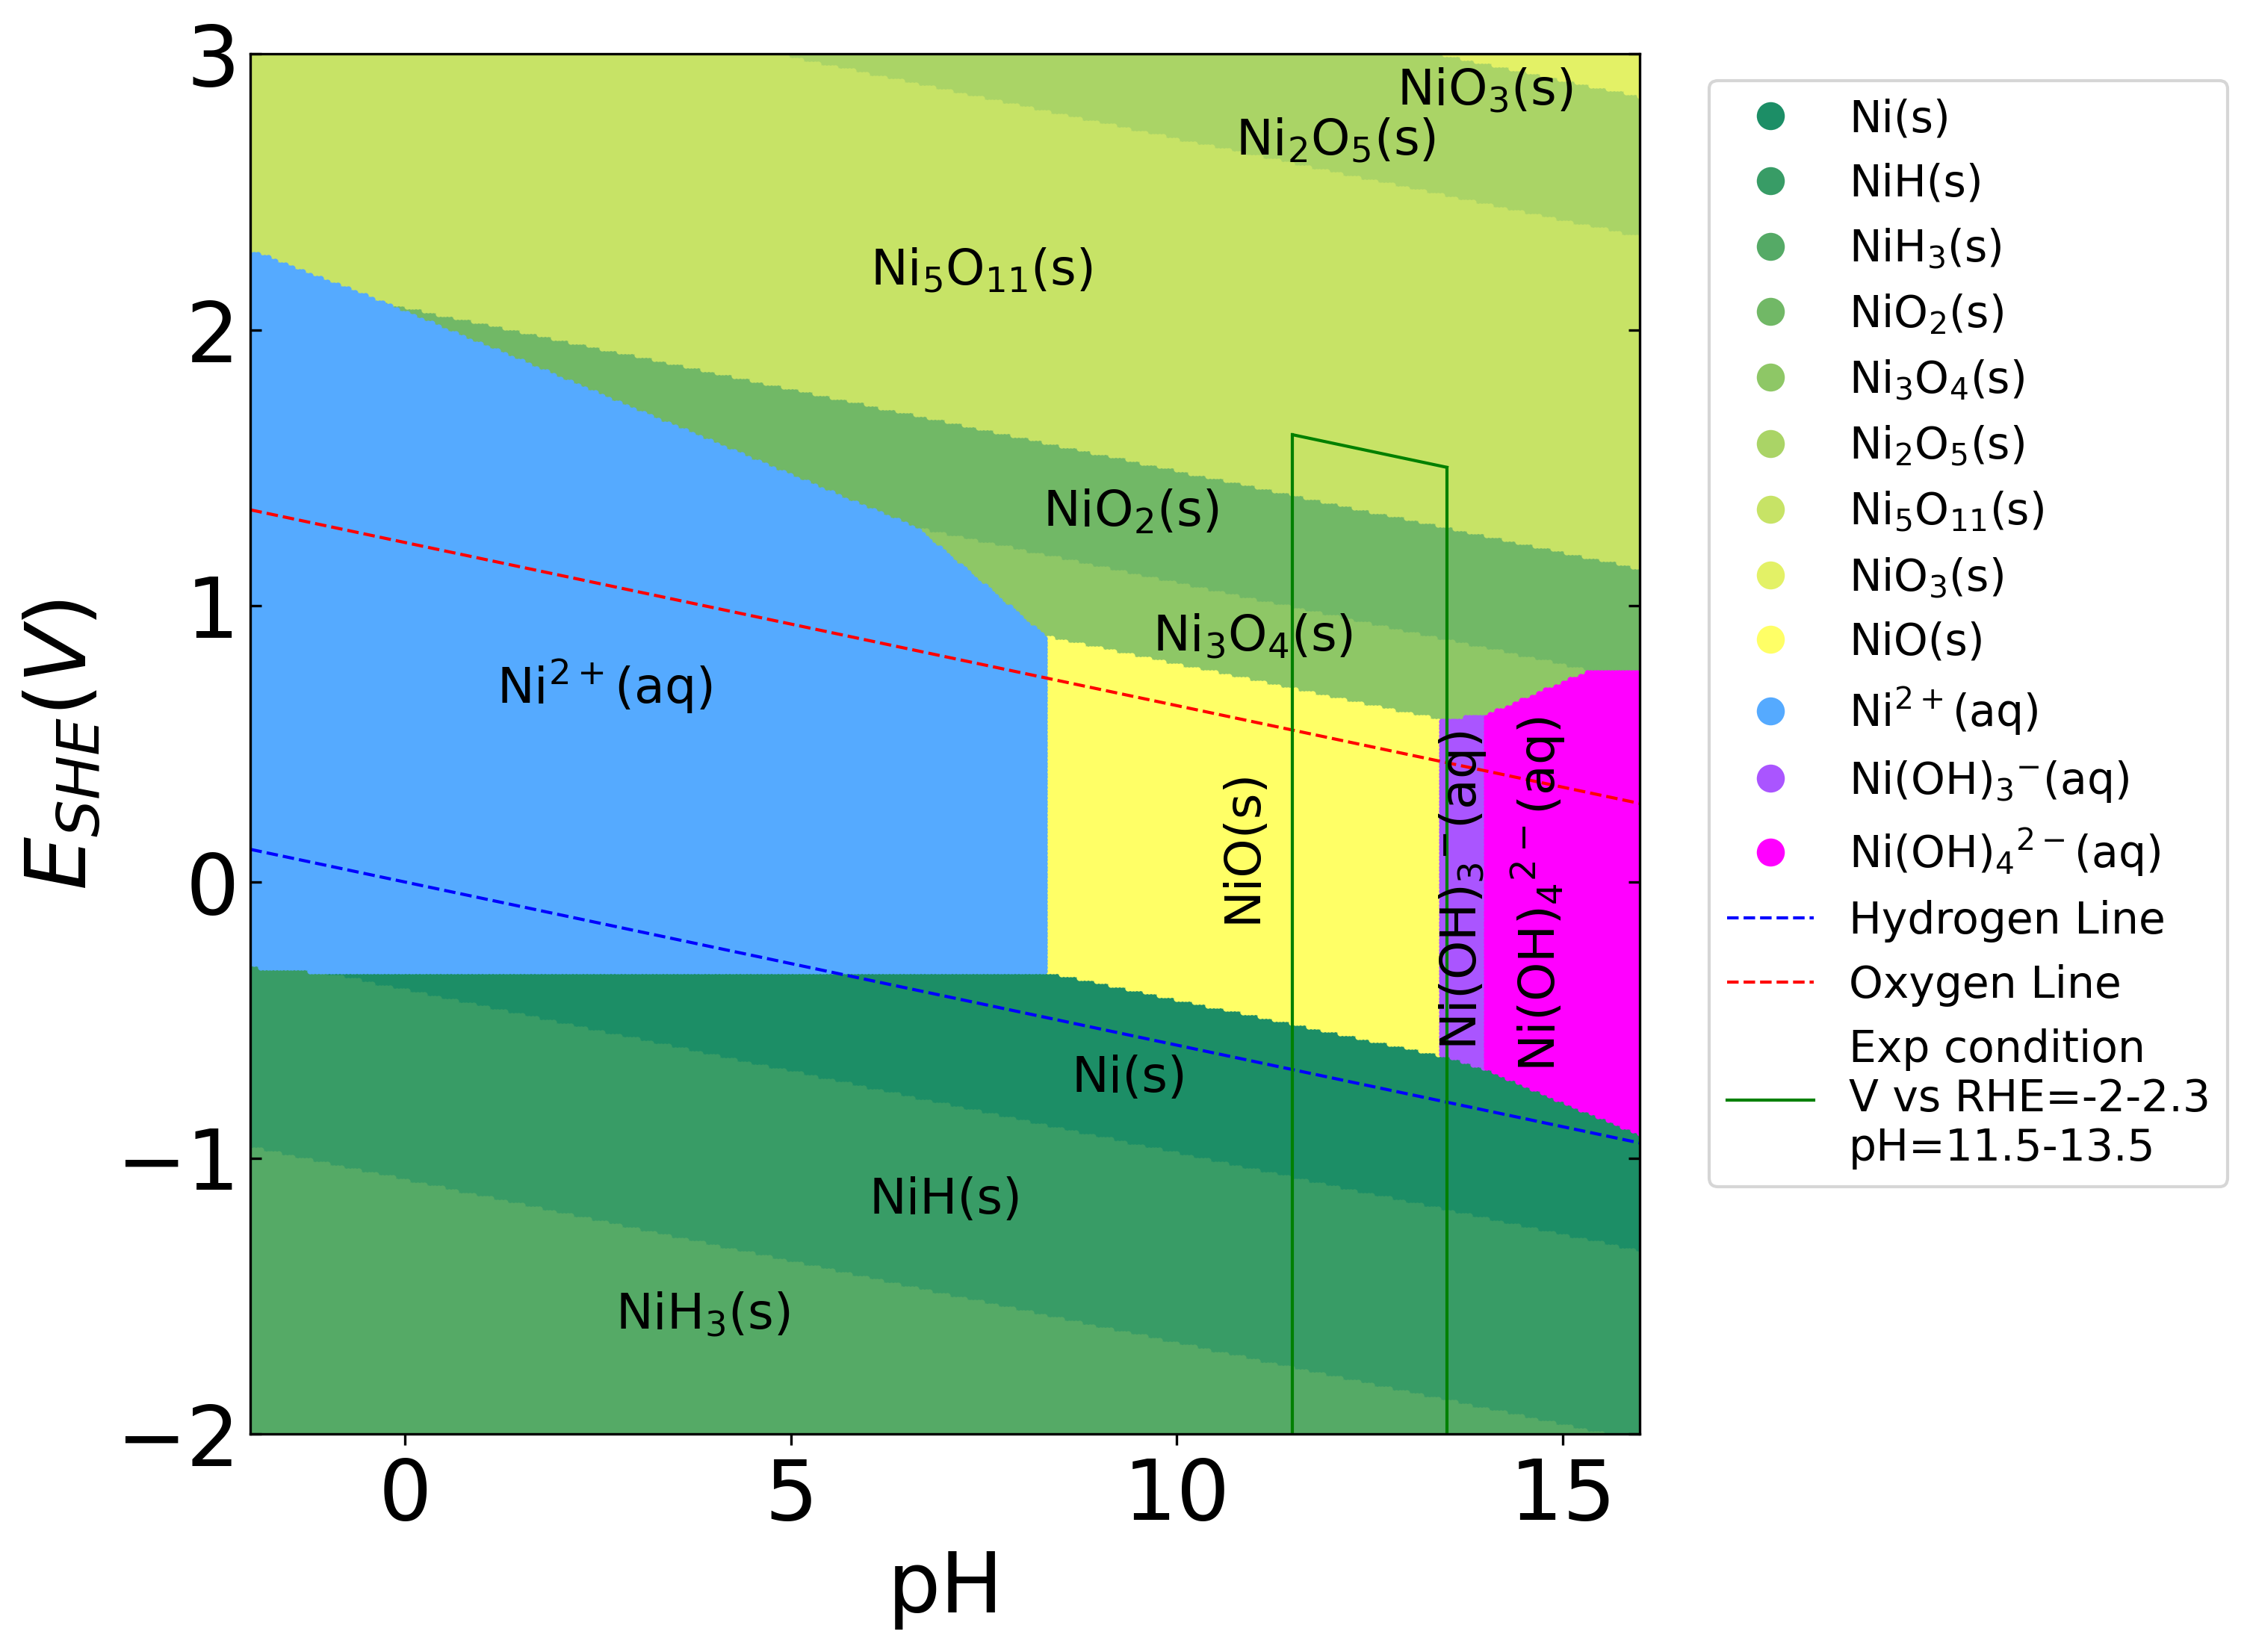
\includegraphics[width=\textwidth]{Figures/pourbaix_diagrams/Ni-NH3-H2O_activity=1e-04_[NH3]=0M_[Gly]=0M_[CN]=0.png}
        \par\medskip
    \end{subfigure}
    \begin{subfigure}[b]{0.3\textwidth}
        \subcaption{}\label{fig:Ni_Pourbaix_NH3_Gly}
        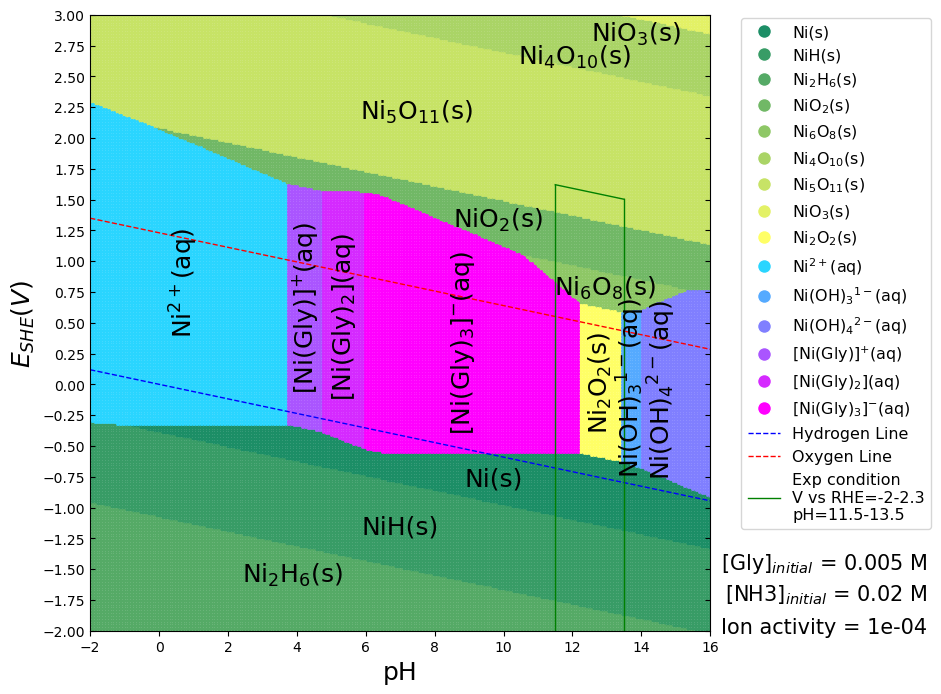
\includegraphics[width=\textwidth]{Figures/pourbaix_diagrams/Ni-NH3-H2O_activity=1e-04_[NH3]=0.02M_[Gly]=0.005M_[CN]=0.png}
        \par\medskip
    \end{subfigure}
    \begin{subfigure}[b]{0.3\textwidth}
        \subcaption{}\label{fig:Ni_Pourbaix_NH3_Gly_CN}
        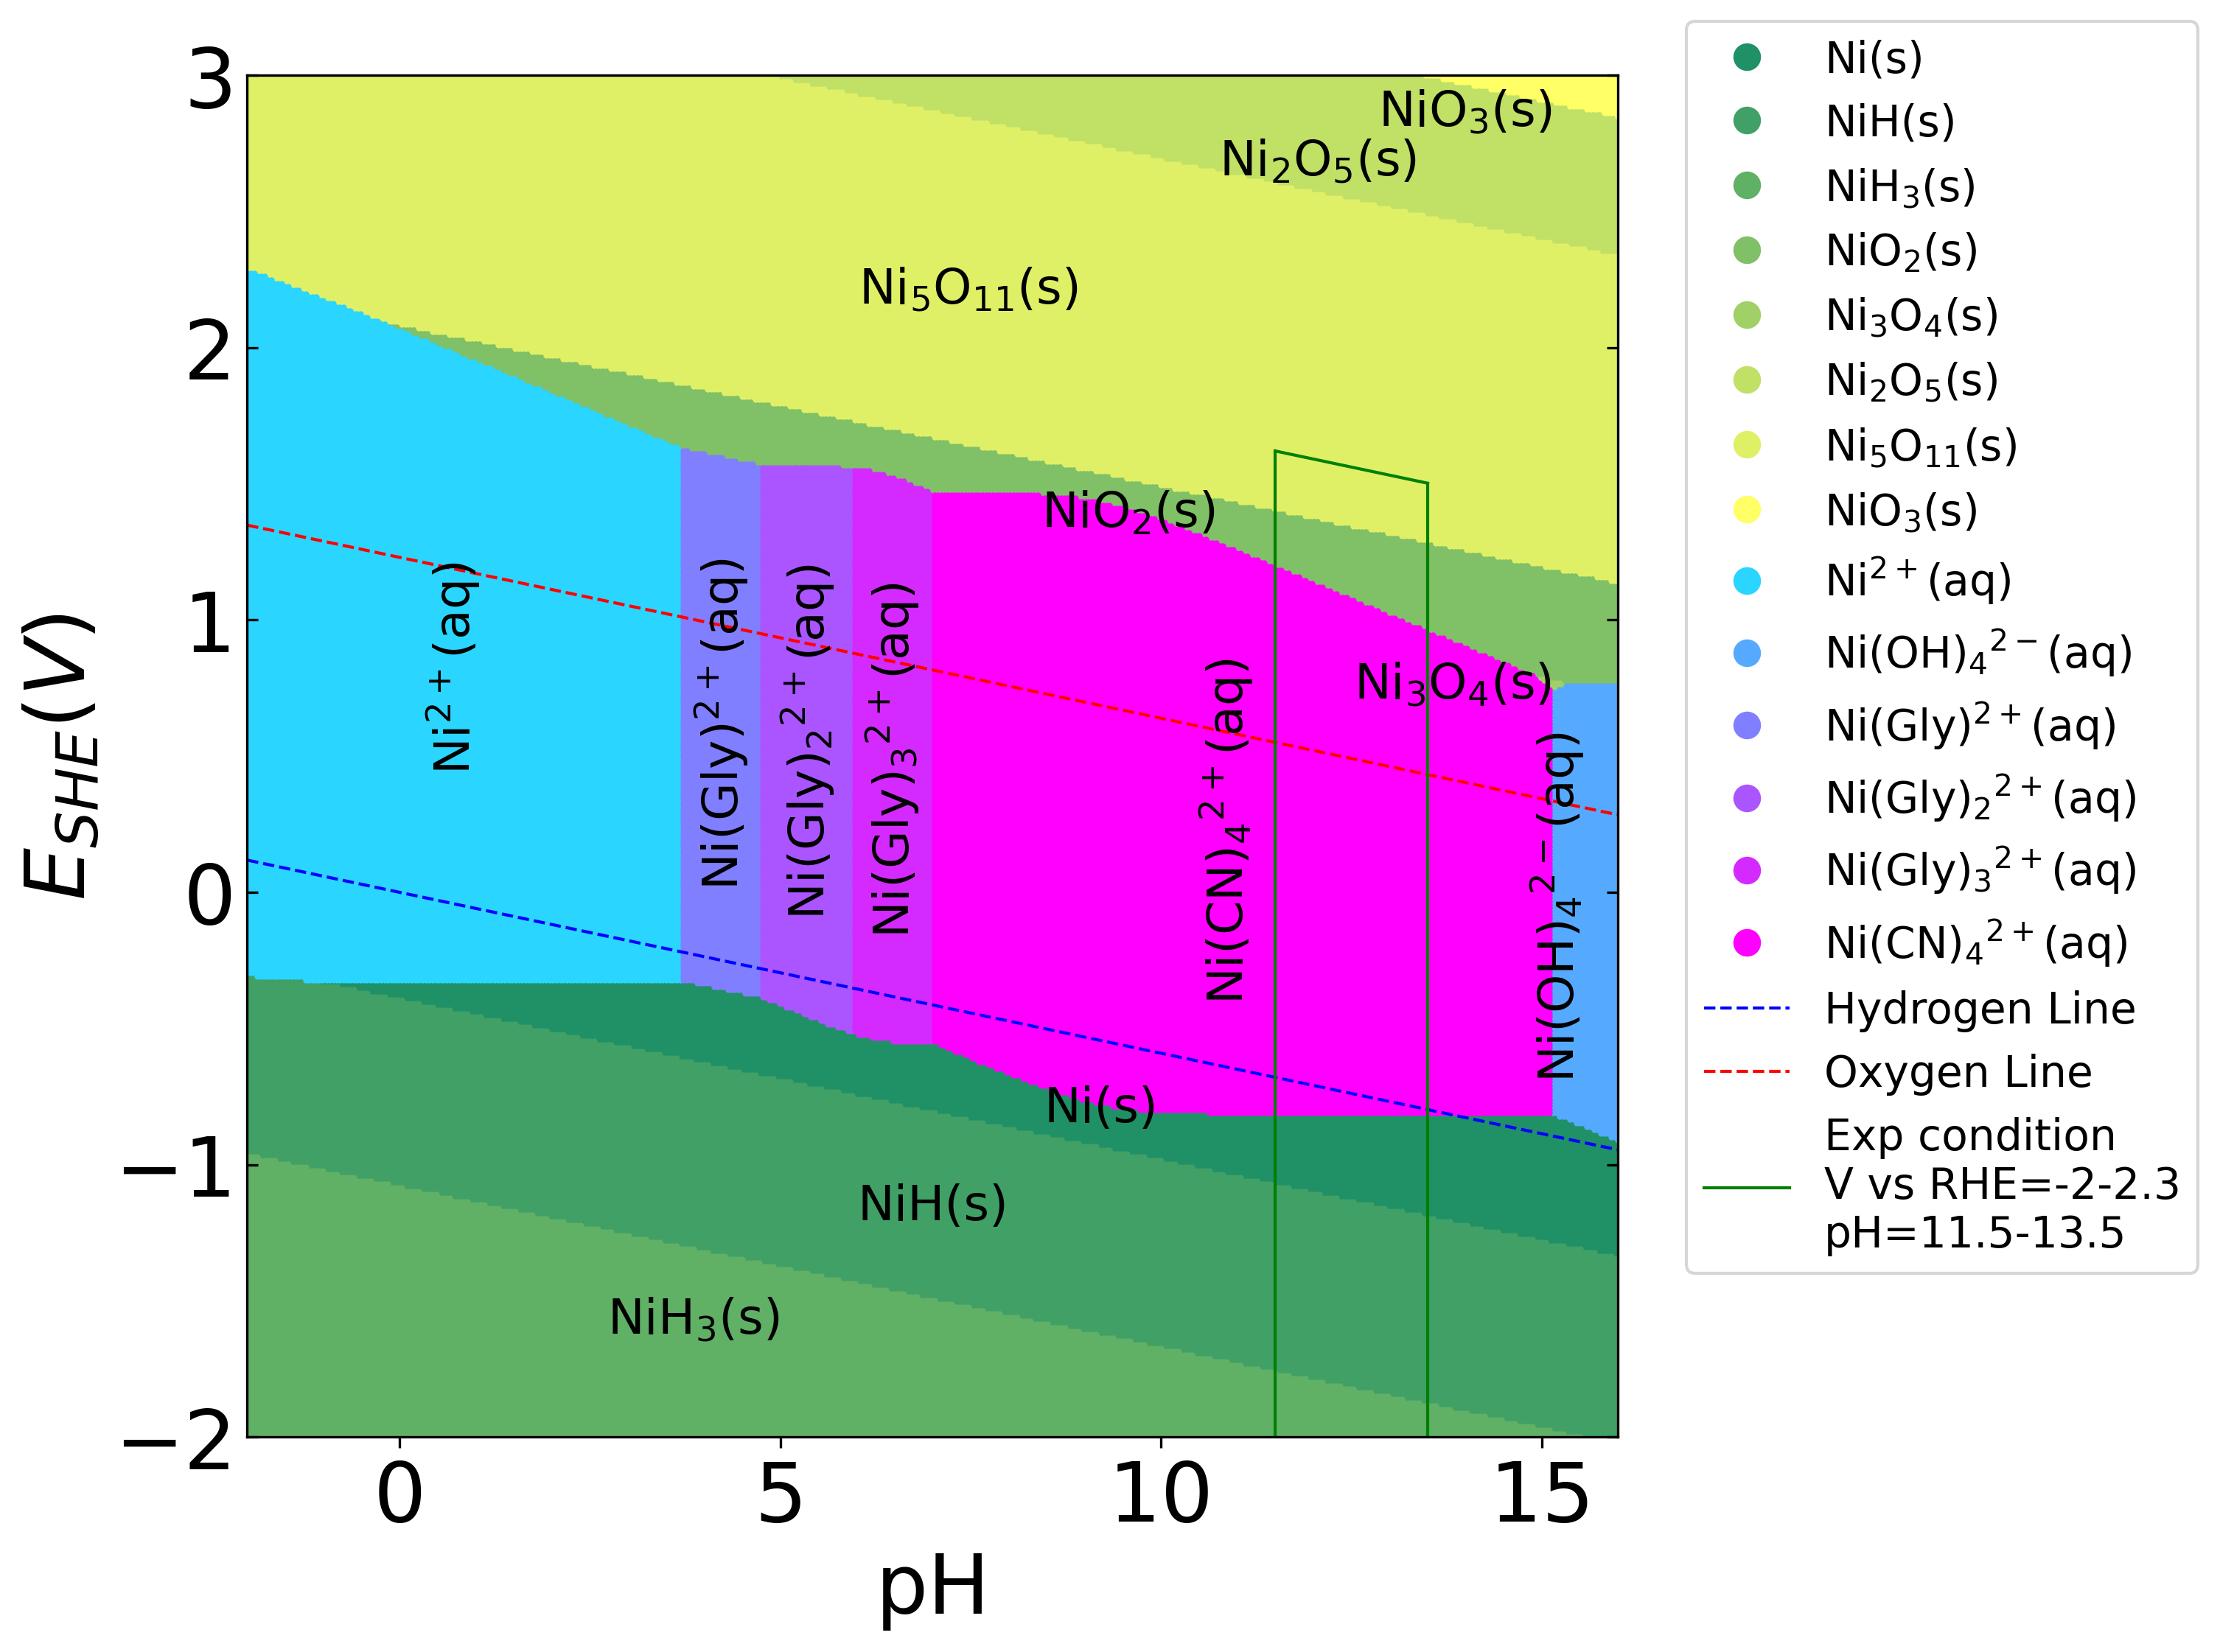
\includegraphics[width=\textwidth]{Figures/pourbaix_diagrams/Ni-NH3-H2O_activity=1e-04_[NH3]=0.02M_[Gly]=0.005M_[CN]=0.0001.png}
        \par\medskip   
    \end{subfigure}
    \caption{Ni Pourbaix diagrams, with $\text{ion activity}=\num{1e-4}$M, (a)\ce{H2O} only, (b)$[\ce{NH3}]_{initial}= 0.02$M, $[\text{Gly}]_{initial}=0.005$M, (c)$[\ce{NH3}]_{initial}= 0.02$M, $[\text{Gly}]_{initial}=0.005$M,  $[\ce{CN-}]_{initial}=\num{1e-4}$M. Green box indicates experimental condition at applied potential vs RHE = -2 to 2V, pH = 11.5 to 13.5.}
    \label{fig:Ni_Pourbaix}
\end{figure}


%%%%%%%%%%%%%%%%%%%%%%%%%%%%%%%%% Cu %%%%%%%%%%%%%%%%%%%%%%%%%%%%%%%%%
\begin{figure}[htbp]
    \centering
    \begin{subfigure}[b]{0.3\textwidth}
        \subcaption{}\label{fig:Cu_Pourbaix_H2O}
        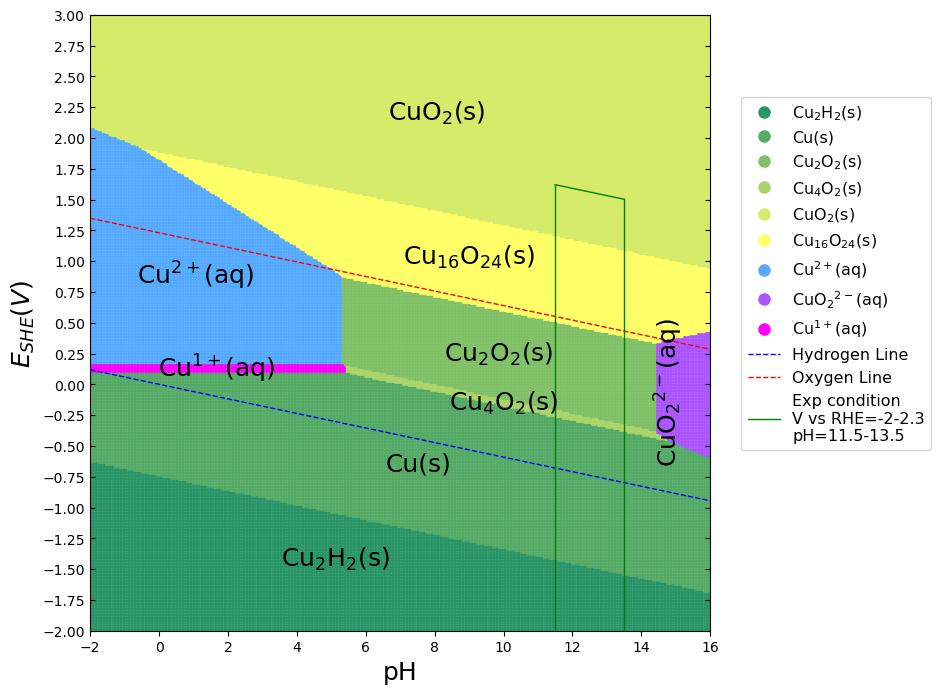
\includegraphics[width=\textwidth]{Figures/pourbaix_diagrams/Cu-NH3-H2O_activity=1e-04_[NH3]=0M_[Gly]=0M_[CN]=0.png}
        \par\medskip
    \end{subfigure}
    \begin{subfigure}[b]{0.3\textwidth}
        \subcaption{}\label{fig:Cu_Pourbaix_NH3_Gly}
        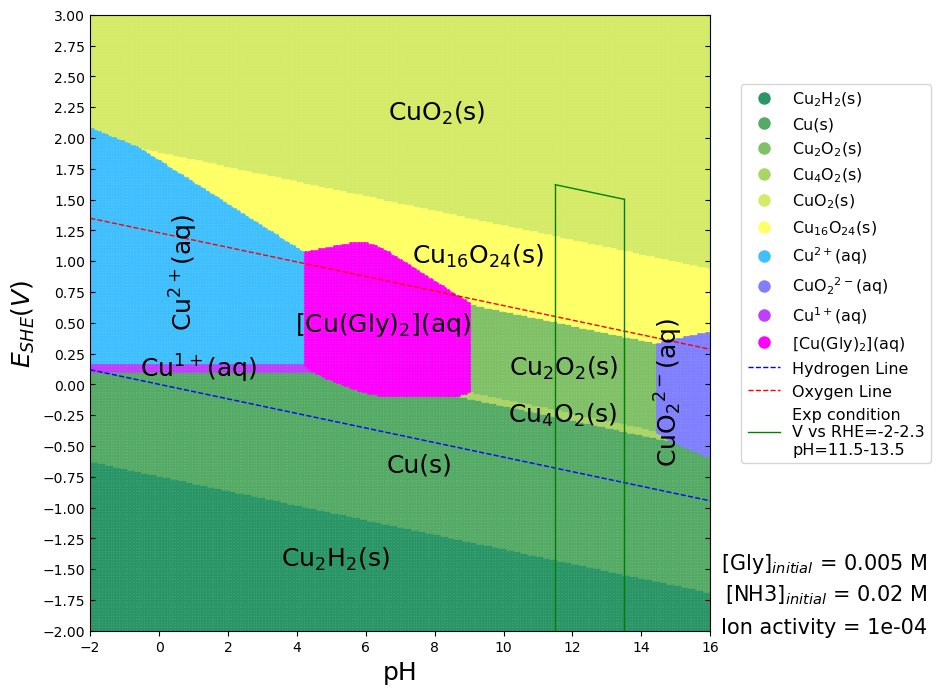
\includegraphics[width=\textwidth]{Figures/pourbaix_diagrams/Cu-NH3-H2O_activity=1e-04_[NH3]=0.02M_[Gly]=0.005M_[CN]=0.png}
        \par\medskip
    \end{subfigure}
    \begin{subfigure}[b]{0.3\textwidth}
        \subcaption{}\label{fig:Cu_Pourbaix_NH3_Gly_CN}
        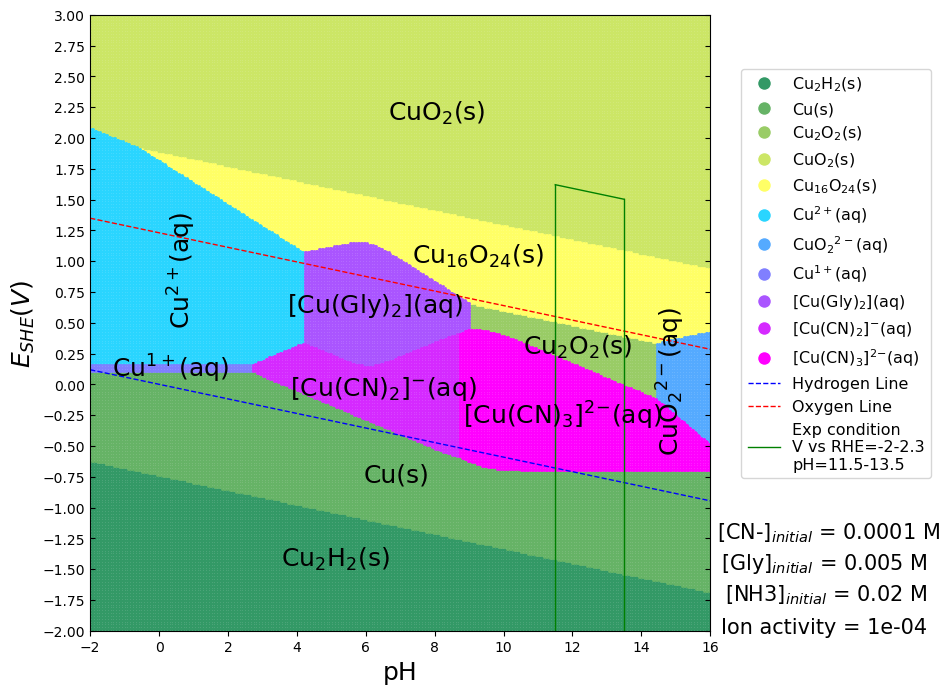
\includegraphics[width=\textwidth]{Figures/pourbaix_diagrams/Cu-NH3-H2O_activity=1e-04_[NH3]=0.02M_[Gly]=0.005M_[CN]=0.0001.png}
        \par\medskip   
    \end{subfigure}
    \caption{Cu Pourbaix diagrams, with $\text{ion activity}=\num{1e-4}$, (a)\ce{H2O} only, (b)$[\ce{NH3}]_{initial}= 0.02$M, $[\text{Gly}]_{initial}=0.005$M, (c)$[\ce{NH3}]_{initial}= 0.02$M, $[\text{Gly}]_{initial}=0.005$M,  $[\ce{CN-}]_{initial}=\num{1e-4}$M. Green box indicates experimental condition at applied potential vs RHE = -2 to 2V, pH = 11.5 to 13.5.}
    \label{fig:Cu_Pourbaix}
\end{figure}

%%%%%%%%%%%%%%%%%%%%%%%%%%%%%%%%% Au %%%%%%%%%%%%%%%%%%%%%%%%%%%%%%%%%
\begin{figure}[htbp]
    \centering
    \begin{subfigure}[b]{0.3\textwidth}
        \subcaption{}\label{fig:Au_Pourbaix_H2O}
        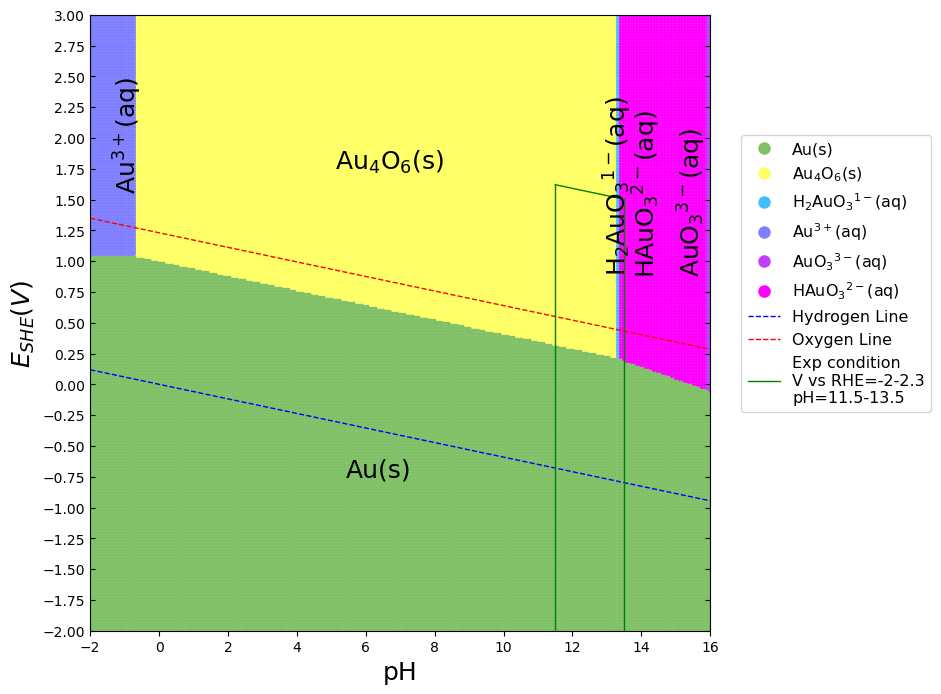
\includegraphics[width=\textwidth]{Figures/pourbaix_diagrams/Au-NH3-H2O_activity=1e-04_[NH3]=0M_[Gly]=0M_[CN]=0.png}
        \par\medskip
    \end{subfigure}
    \begin{subfigure}[b]{0.3\textwidth}
        \subcaption{}\label{fig:Au_Pourbaix_NH3_Gly}
        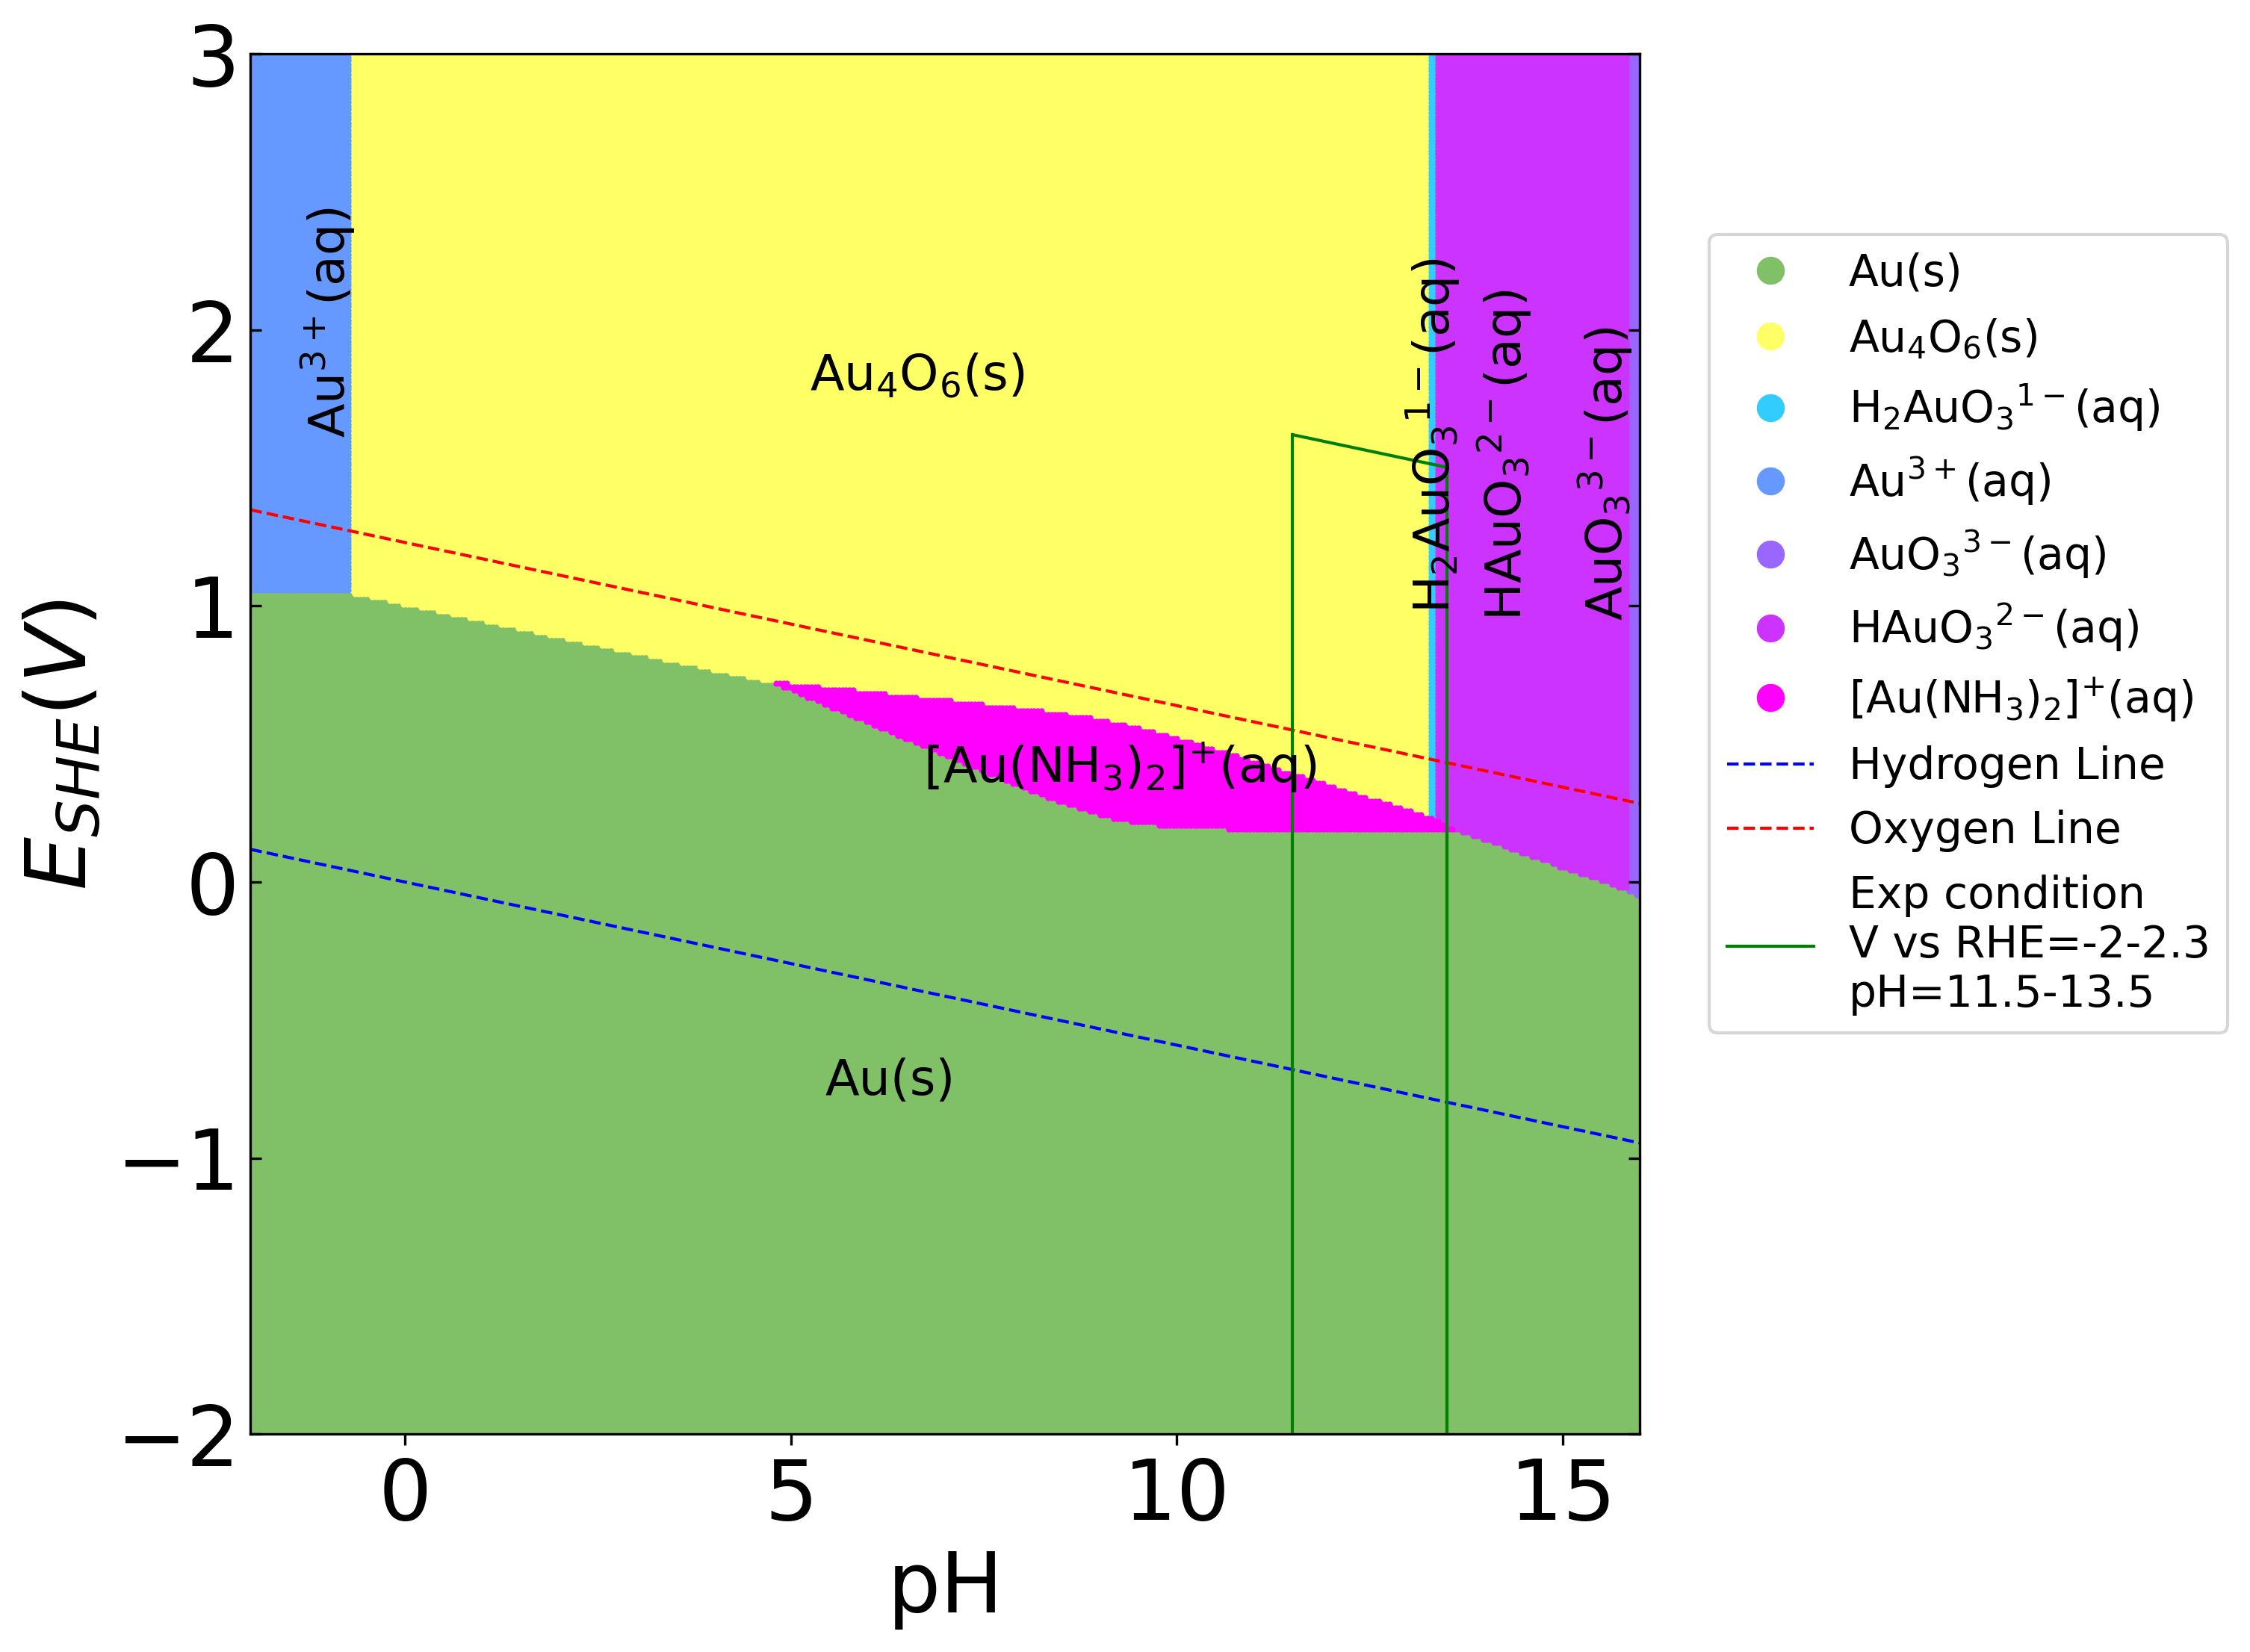
\includegraphics[width=\textwidth]{Figures/pourbaix_diagrams/Au-NH3-H2O_activity=1e-04_[NH3]=0.02M_[Gly]=0.005M_[CN]=0.png}
        \par\medskip
    \end{subfigure}
    \begin{subfigure}[b]{0.3\textwidth}
        \subcaption{}\label{fig:Au_Pourbaix_NH3_Gly_CN}
        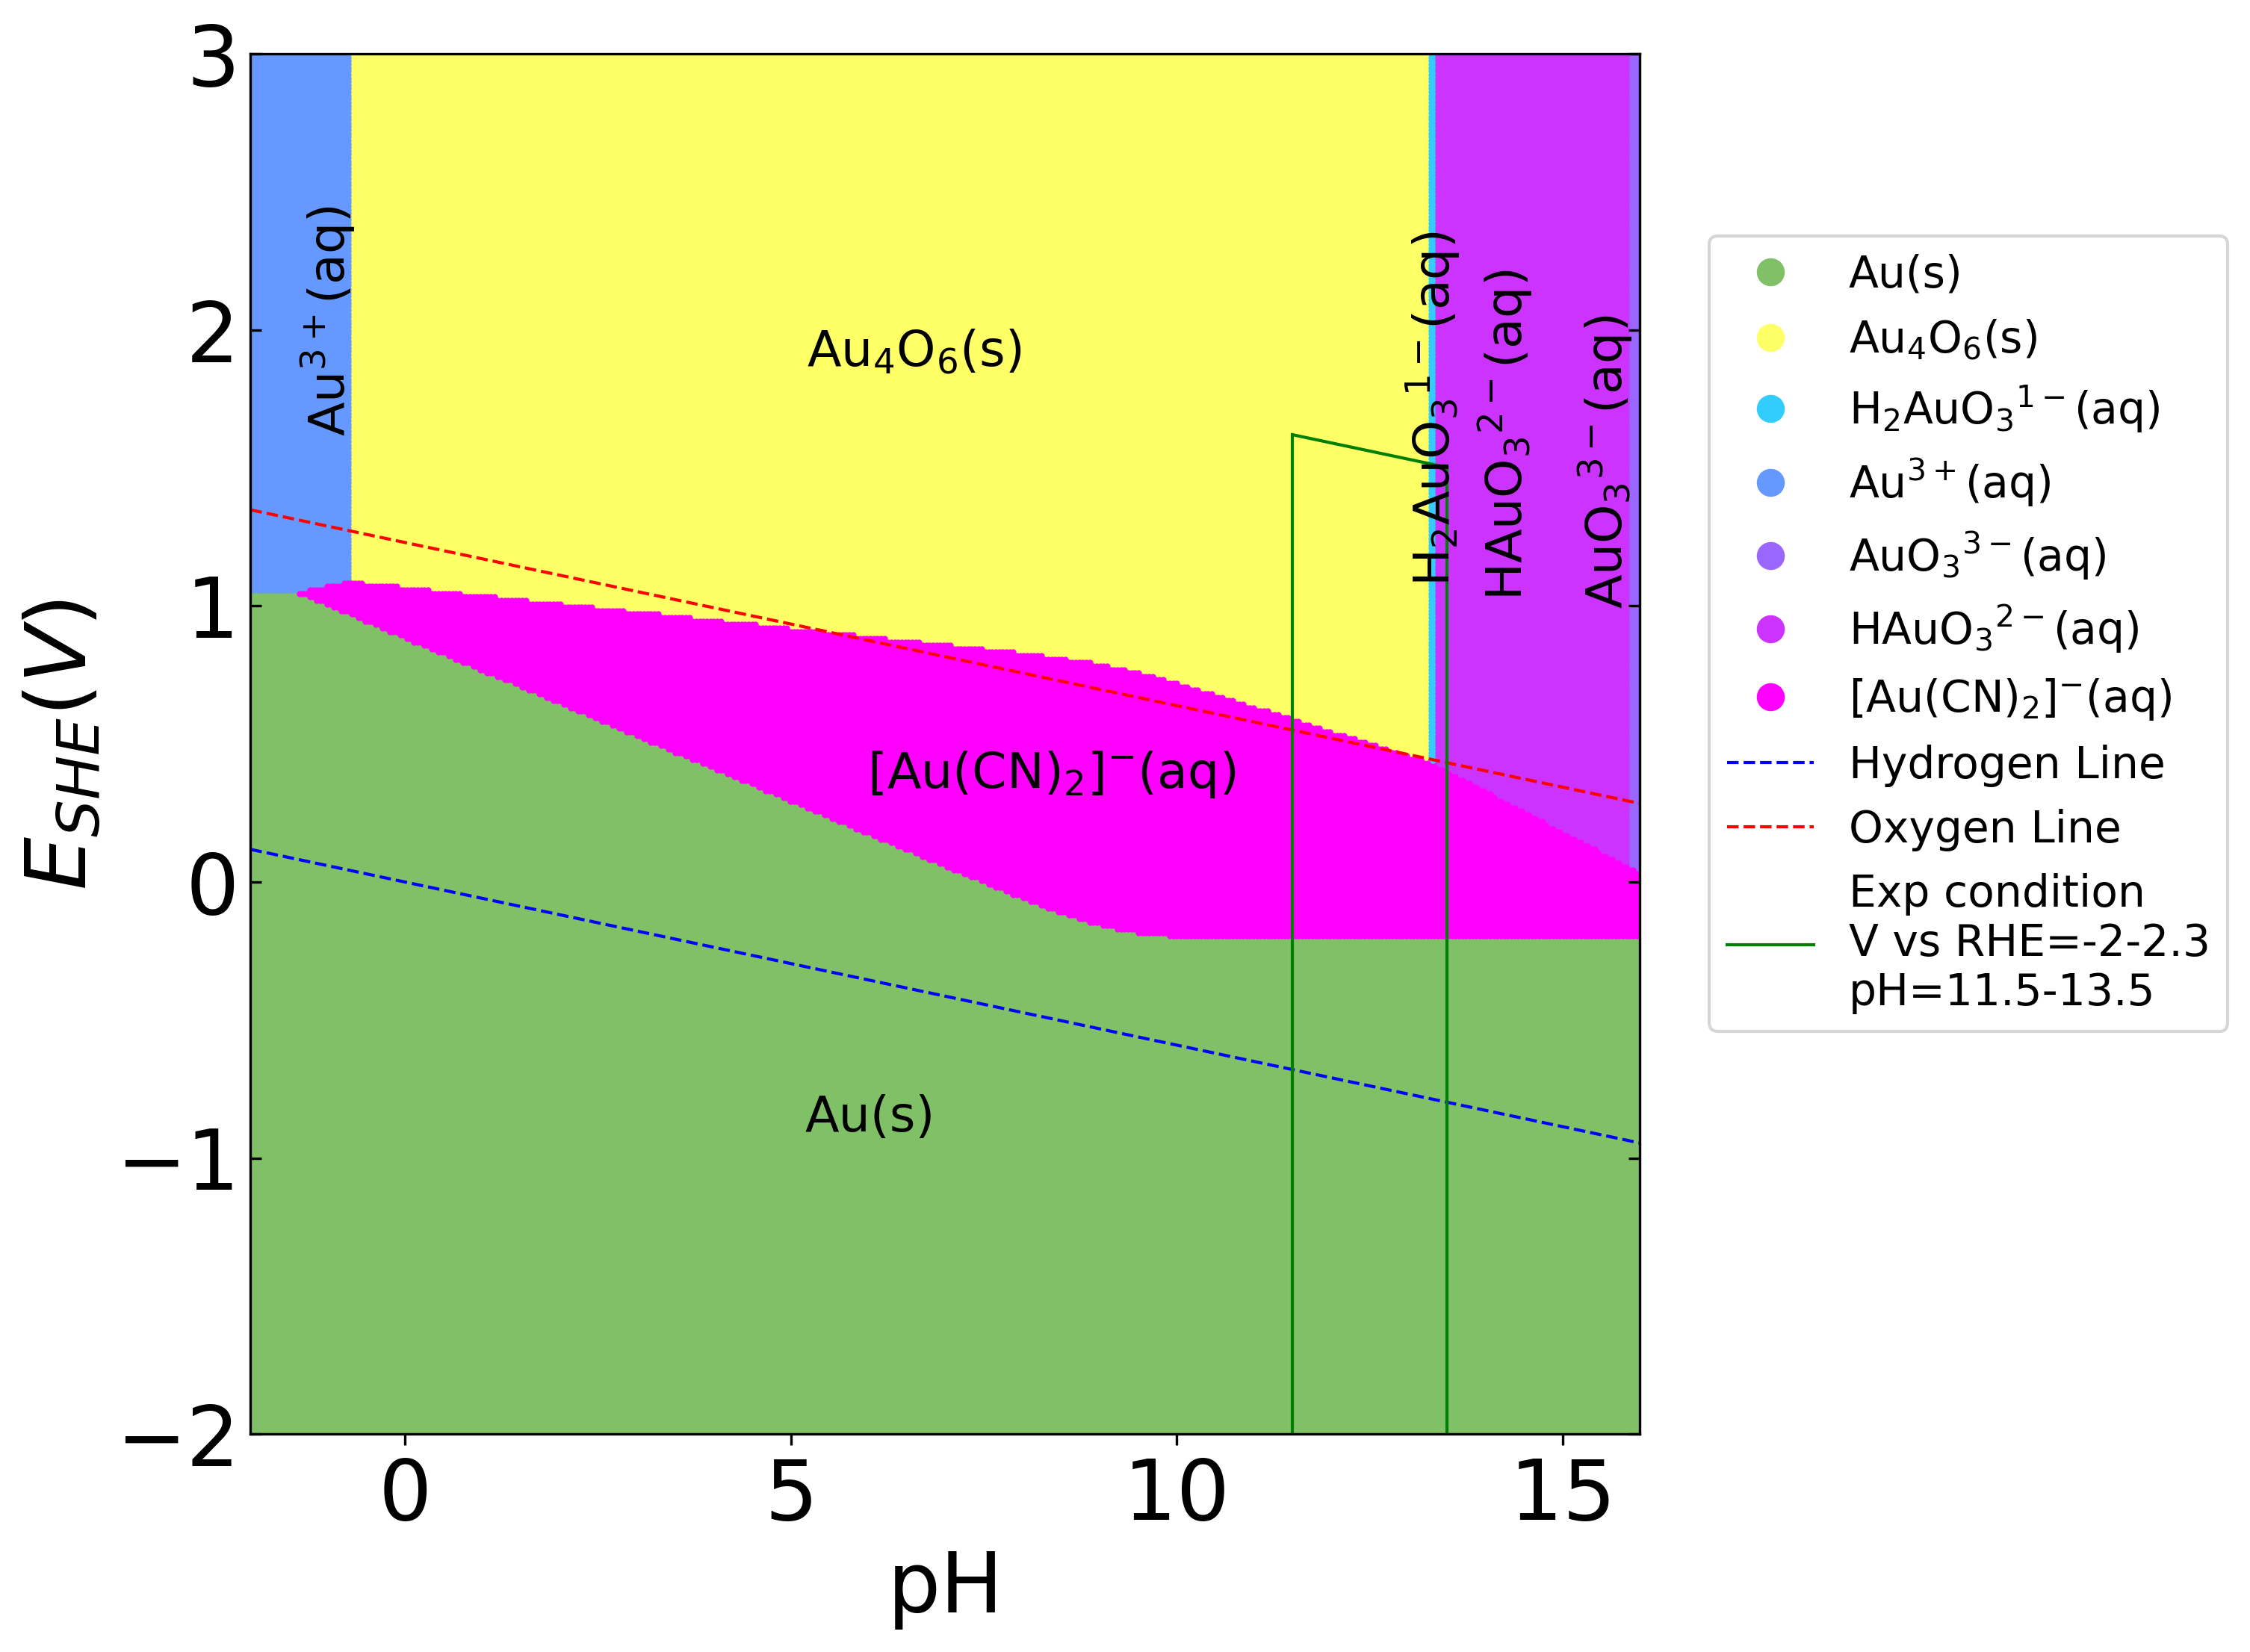
\includegraphics[width=\textwidth]{Figures/pourbaix_diagrams/Au-NH3-H2O_activity=1e-04_[NH3]=0.02M_[Gly]=0.005M_[CN]=0.0001.png}
        \par\medskip   
    \end{subfigure}
    \caption{Au Pourbaix diagrams, with $\text{ion activity}=\num{1e-4}$, (a)\ce{H2O} only, (b)$[\ce{NH3}]_{initial}= 0.02$M, $[\text{Gly}]_{initial}=0.005$M, (c)$[\ce{NH3}]_{initial}= 0.02$M, $[\text{Gly}]_{initial}=0.005$M,  $[\ce{CN-}]_{initial}=\num{1e-4}$M. Green box indicates experimental condition at applied potential vs RHE = -2 to 2V, pH = 11.5 to 13.5.}
    \label{fig:Au_Pourbaix}
\end{figure}
%%%%%%%%%%%%%%%%%%%%%%%%%%%%%%%%% Pd %%%%%%%%%%%%%%%%%%%%%%%%%%%%%%%%%
\begin{figure}[htbp]
    \centering
    \begin{subfigure}[b]{0.45\textwidth}
        \subcaption{}\label{fig:Pd_Pourbaix_NH3_Gly}
        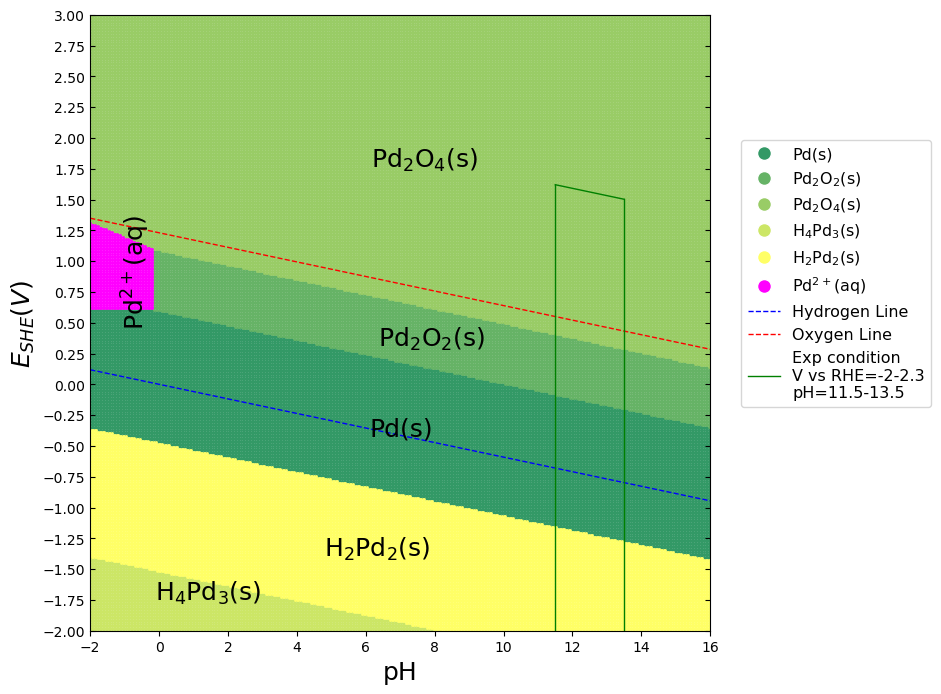
\includegraphics[width=\textwidth]{Figures/pourbaix_diagrams/Pd-NH3-H2O_activity=1e-04_[NH3]=0.02M_[Gly]=0.005M_[CN]=0.png}
        \par\medskip
    \end{subfigure}
    \begin{subfigure}[b]{0.45\textwidth}
        \subcaption{}\label{fig:Pd_Pourbaix_NH3_Gly_CN}
        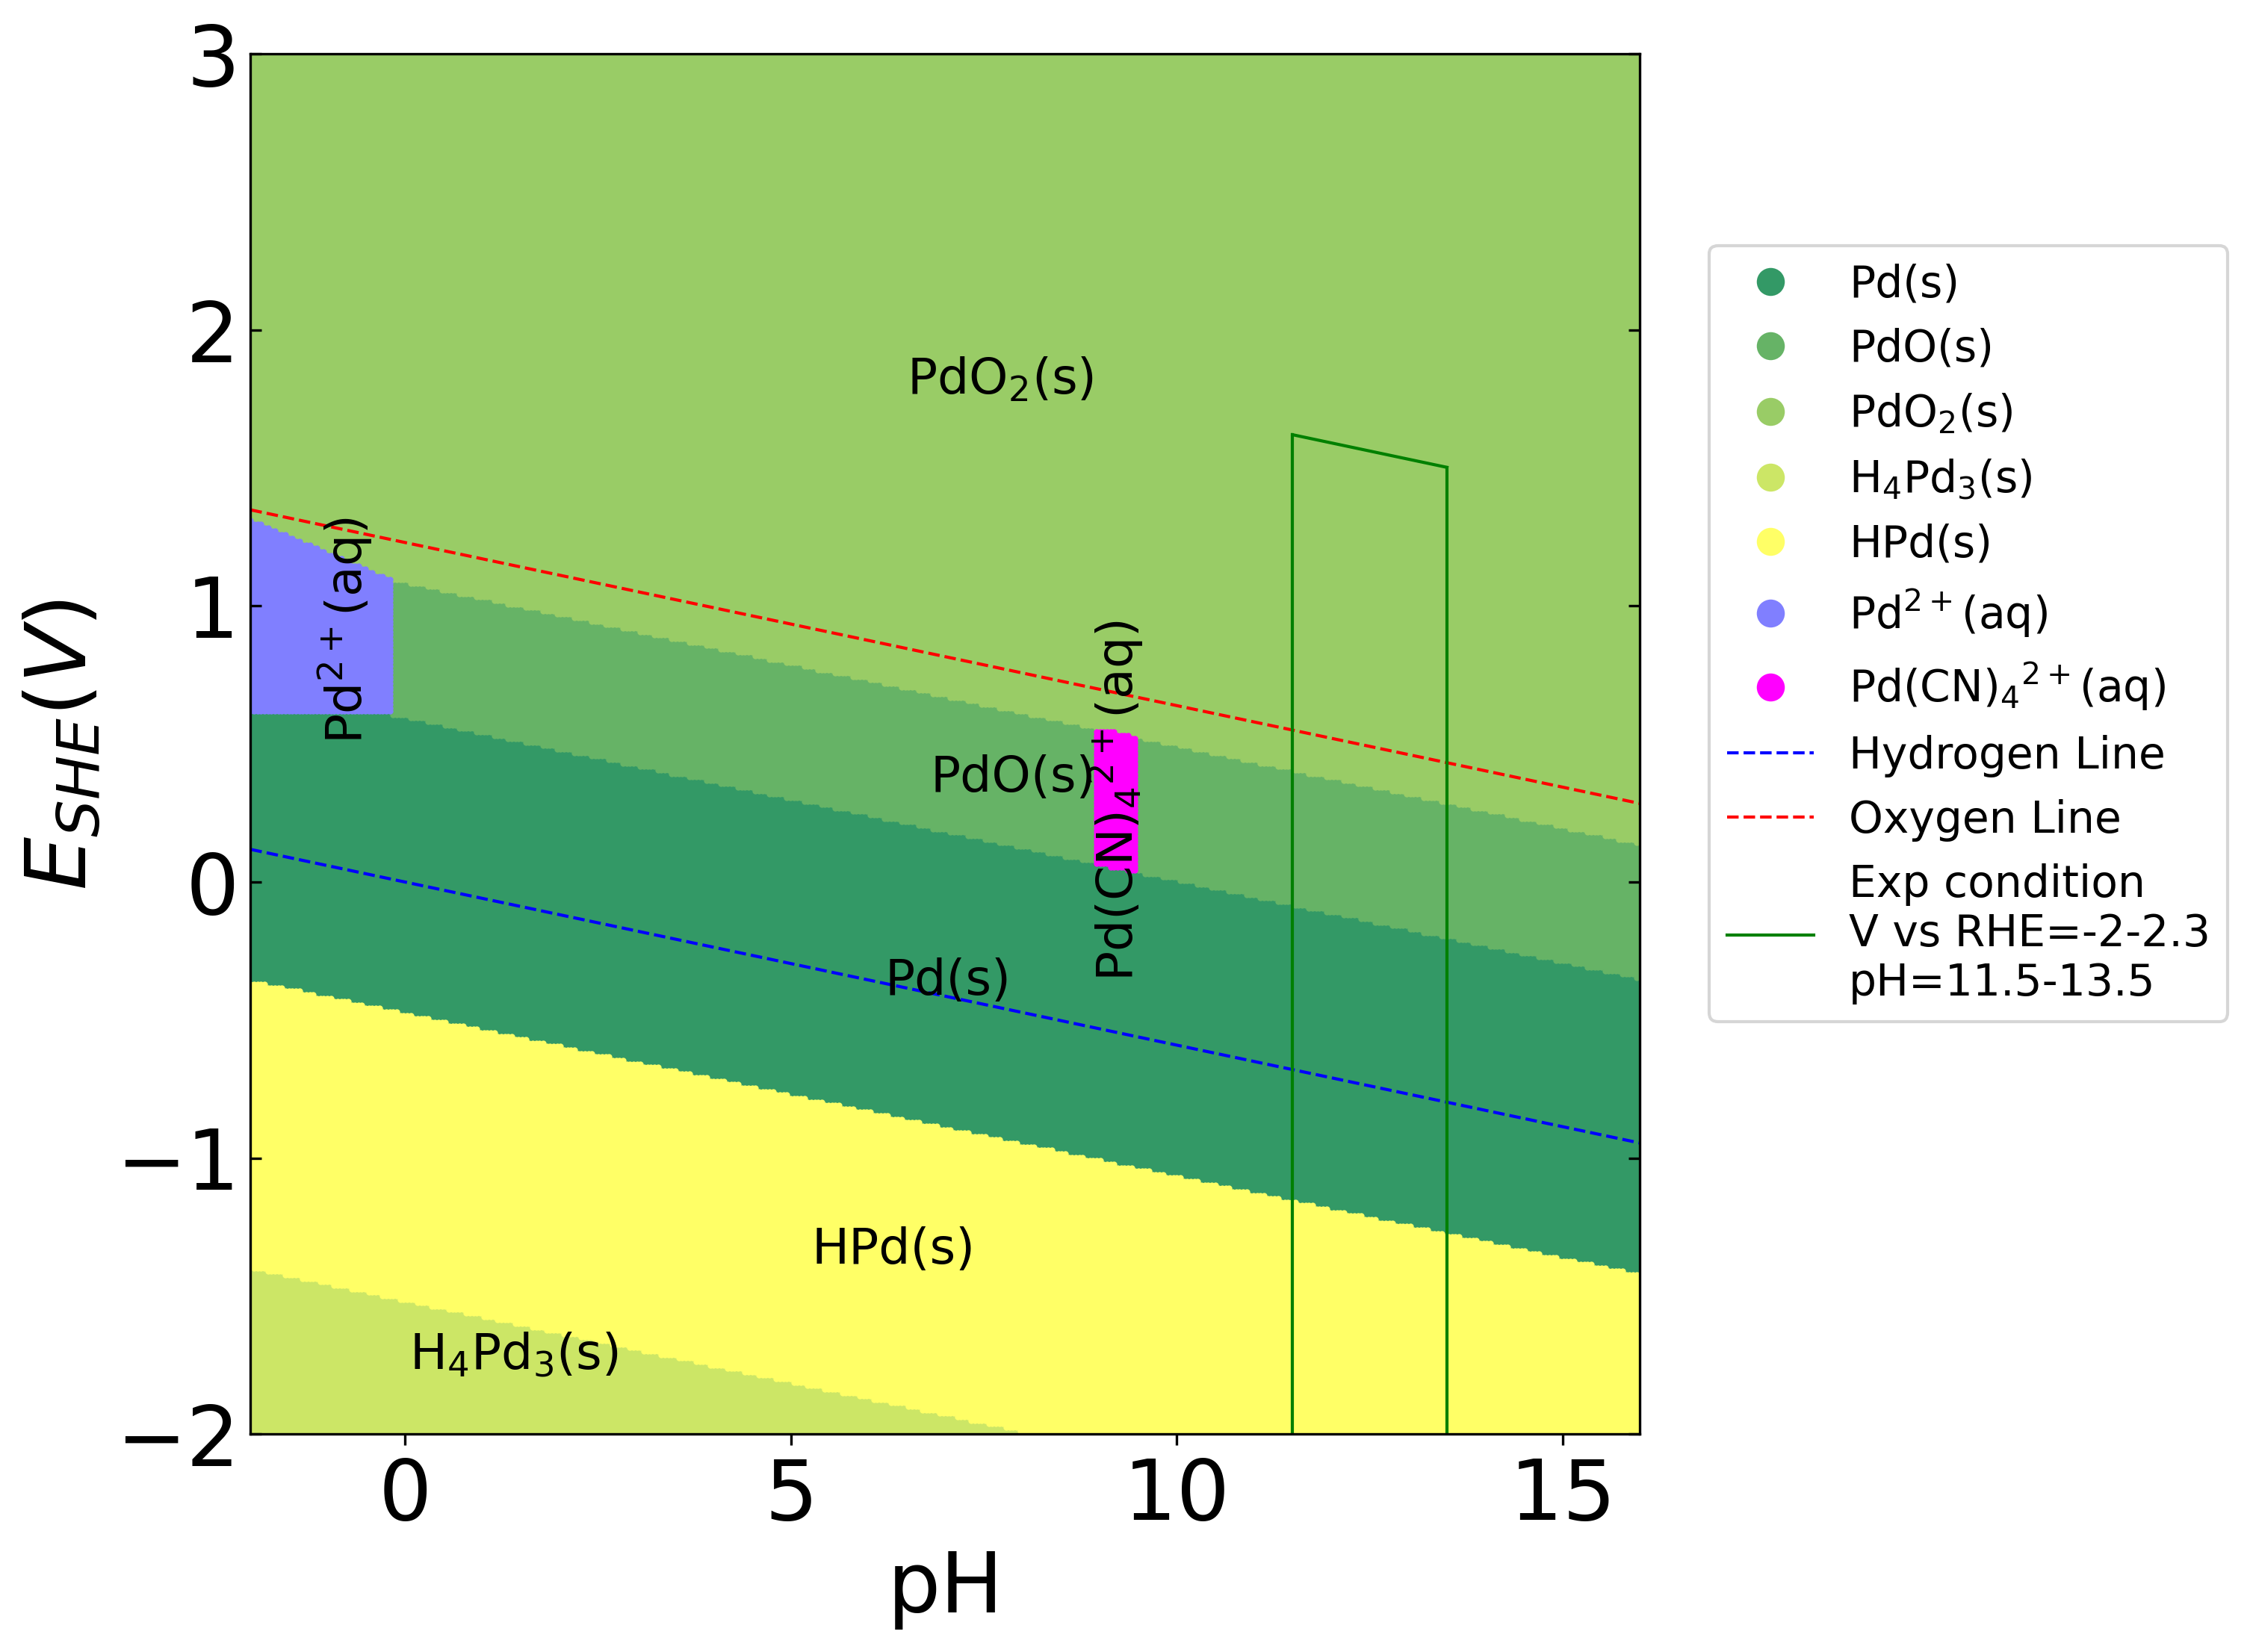
\includegraphics[width=\textwidth]{Figures/pourbaix_diagrams/Pd-NH3-H2O_activity=1e-04_[NH3]=0.02M_[Gly]=0.005M_[CN]=0.0001.png}
        \par\medskip   
    \end{subfigure}

    \caption{Pd Pourbaix diagrams, with $\text{ion activity}=\num{1e-4}$, (a)$[\ce{NH3}]_{initial}= 0.02$M, $[\text{Gly}]_{initial}=0.005$M, (b)$[\ce{NH3}]_{initial}= 0.02$M, $[\text{Gly}]_{initial}=0.005$M,  $[\ce{CN-}]_{initial}=\num{1e-4}$M. Green box indicates experimental condition at applied potential vs RHE = -2 to 2V, pH = 11.5 to 13.5.}
    \label{fig:Pd_Pourbaix}
\end{figure}

%%%%%%%%%%%%%%%%%%%%%%%%%%%%%%%%% Pt and Ti %%%%%%%%%%%%%%%%%%%%%%%%%%%%%%%%%
\begin{figure}[htbp]
    \centering
    \begin{subfigure}[b]{0.45\textwidth}
        \subcaption{}\label{fig:Ti_Pourbaix_NH3_Gly_CN}
        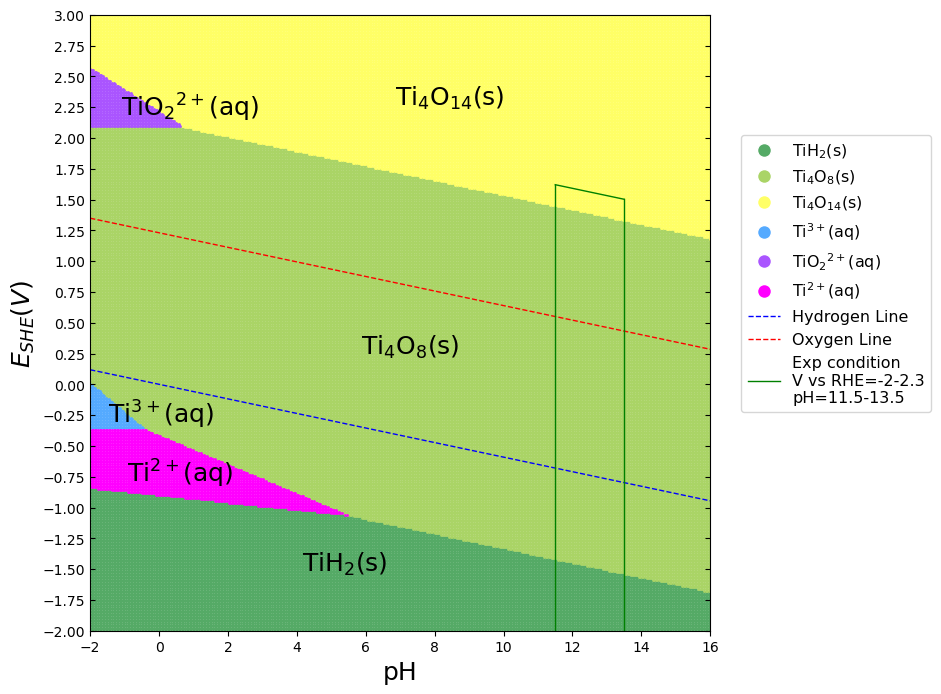
\includegraphics[width=\textwidth]{Figures/pourbaix_diagrams/Ti-NH3-H2O_activity=1e-04_[NH3]=0.02M_[Gly]=0.005M_[CN]=0.0001.png}
        \par\medskip
    \end{subfigure}
    \begin{subfigure}[b]{0.45\textwidth}
        \subcaption{}\label{fig:Pt_Pourbaix_NH3_Gly_CN}
        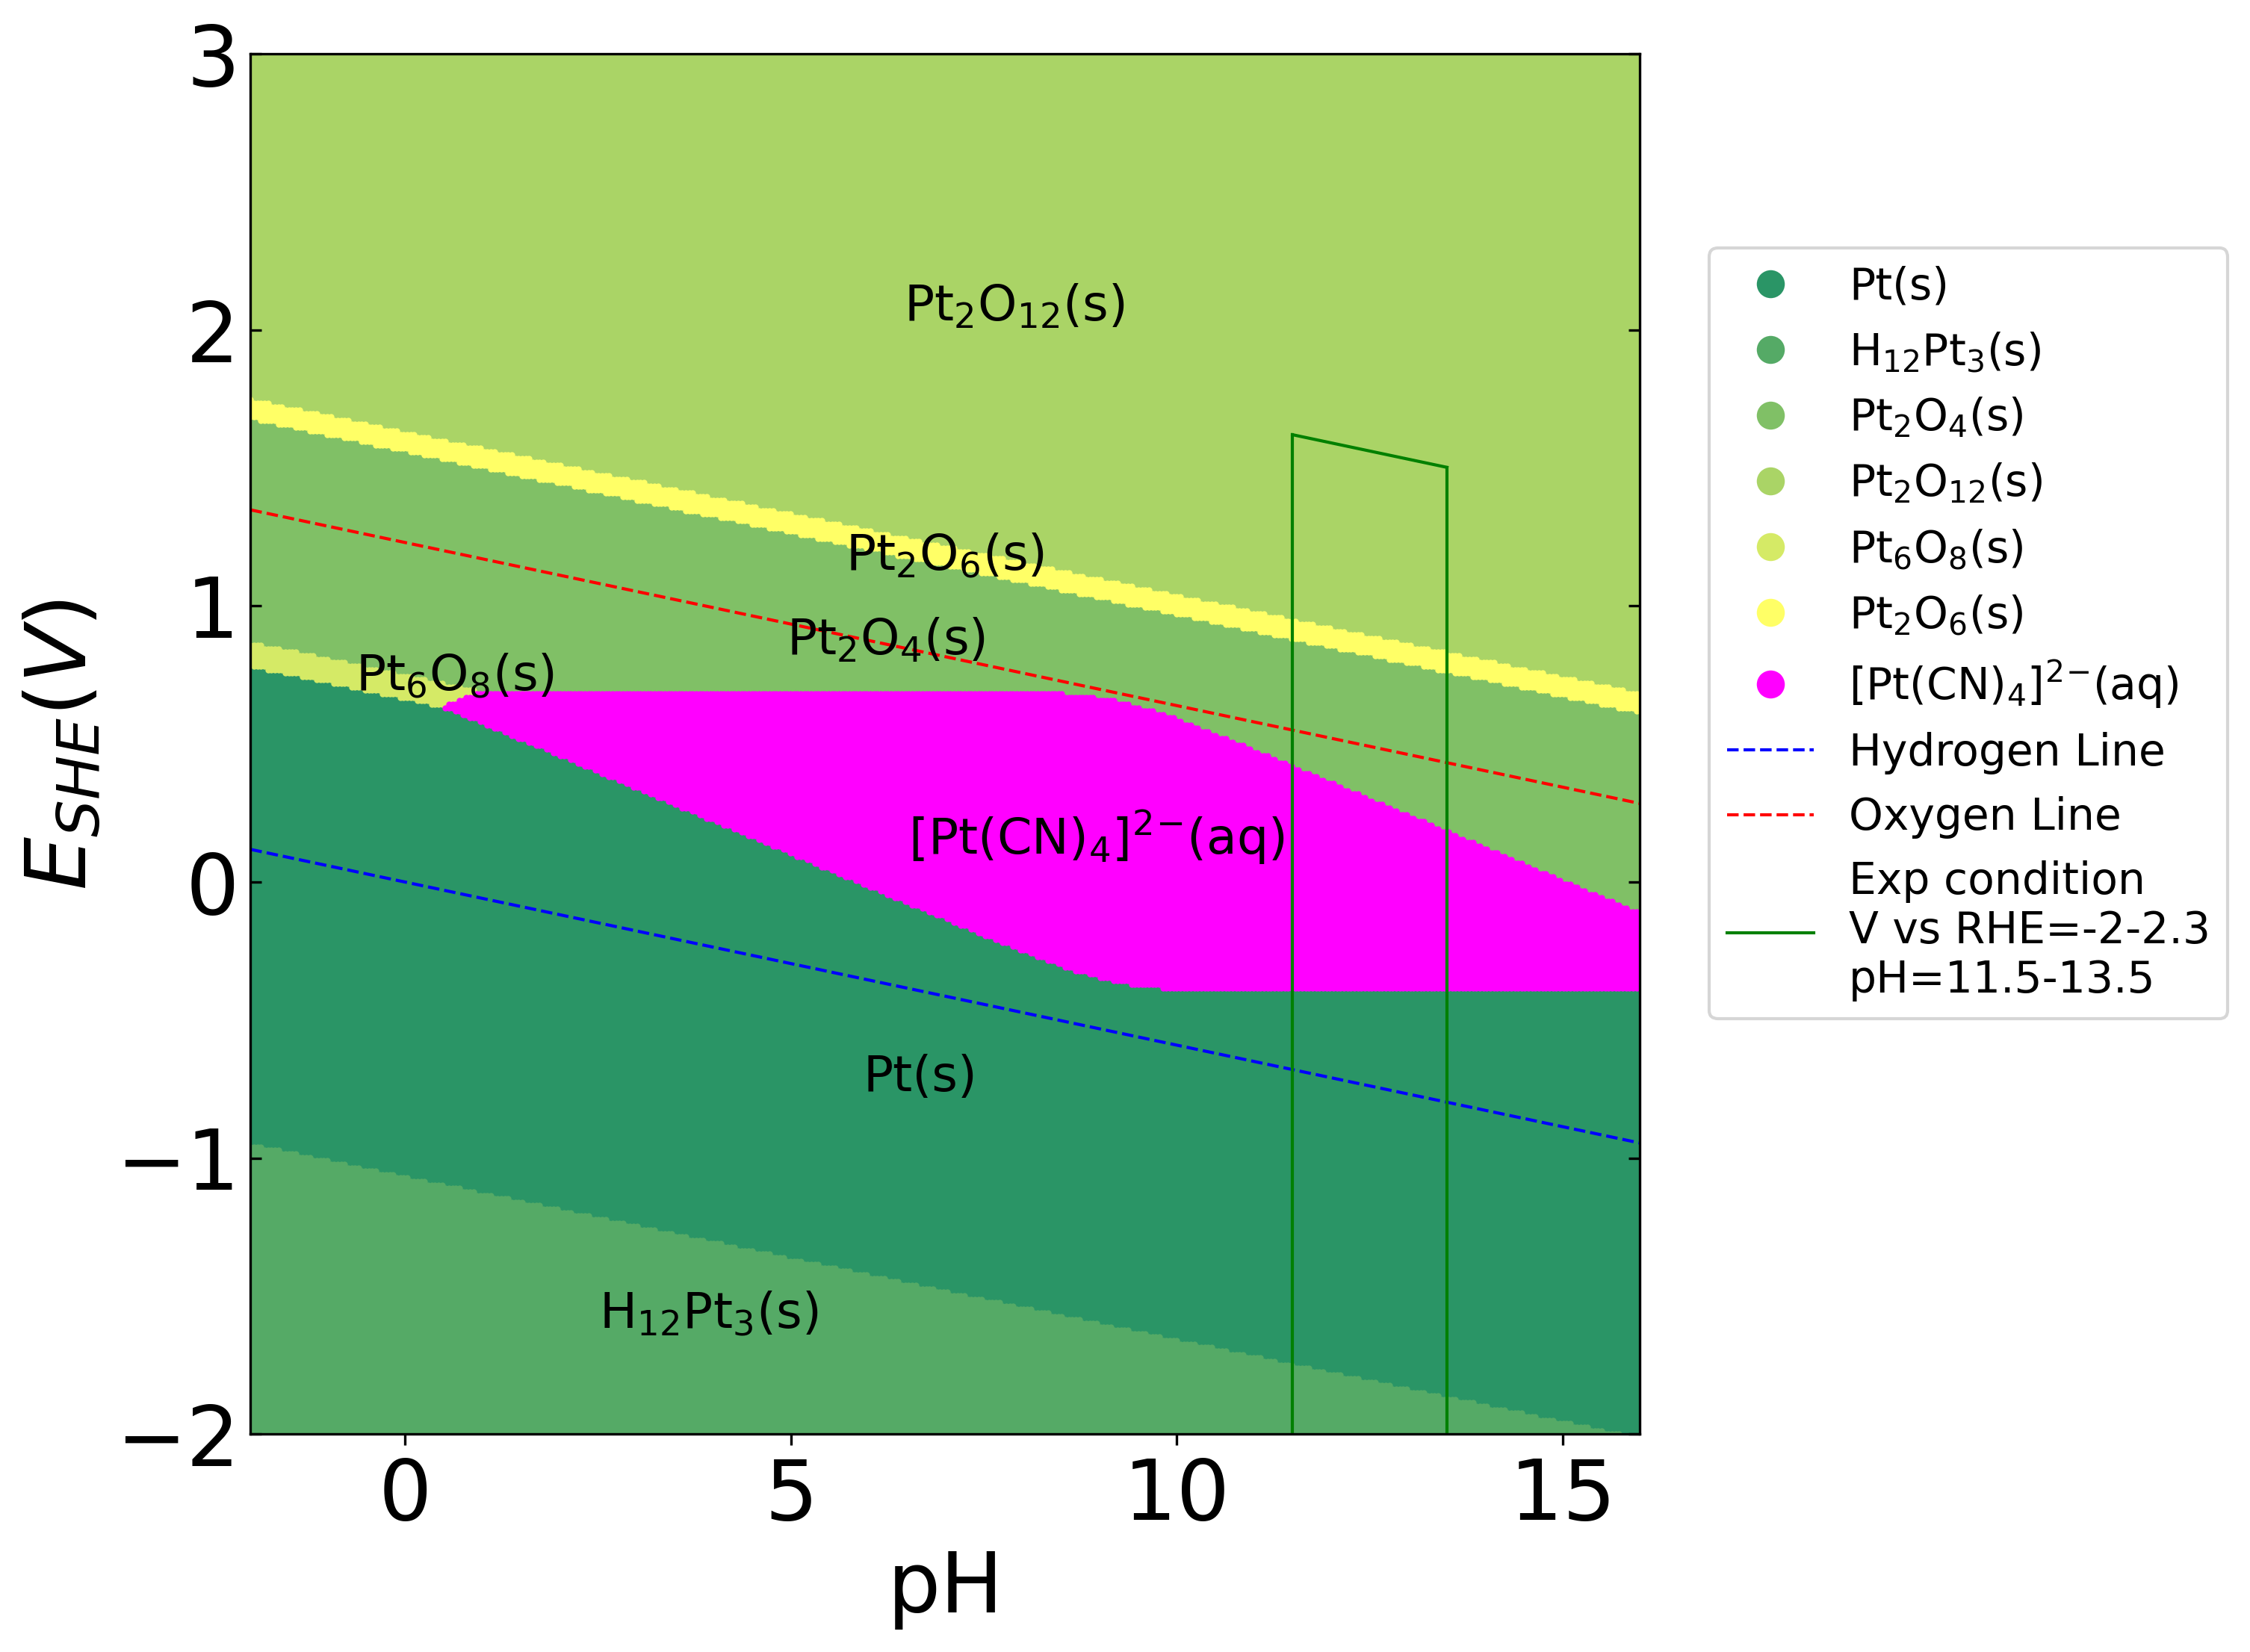
\includegraphics[width=\textwidth]{Figures/pourbaix_diagrams/Pt-NH3-H2O_activity=1e-04_[NH3]=0.02M_[Gly]=0.005M_[CN]=0.0001.png}
        \par\medskip   
    \end{subfigure}
    \caption{Pourbaix diagrams of (a) Ti, (b) Pt. $\text{Ion activity}=\num{1e-4}$, $[\ce{NH3}]_{initial}= 0.02$M, $[\text{Gly}]_{initial}=0.005$M,  $[\ce{CN-}]_{initial}=\num{1e-4}$M. Green box indicates experimental condition at applied potential vs RHE = -2 to 2V, pH = 11.5 to 13.5.}
    \label{fig:Ti_Pt_Pourbaix}
\end{figure}


%%%%%%%%%%%%%%%%%%%%%%%%%%%%%%%%% TiNi Alloy %%%%%%%%%%%%%%%%%%%%%%%%%%%%%%%%%
\begin{figure}[htbp]
    \centering
    \begin{subfigure}[b]{0.45\textwidth}
        \subcaption{}\label{fig:TiNi_Pourbaix_NH3_Gly}
        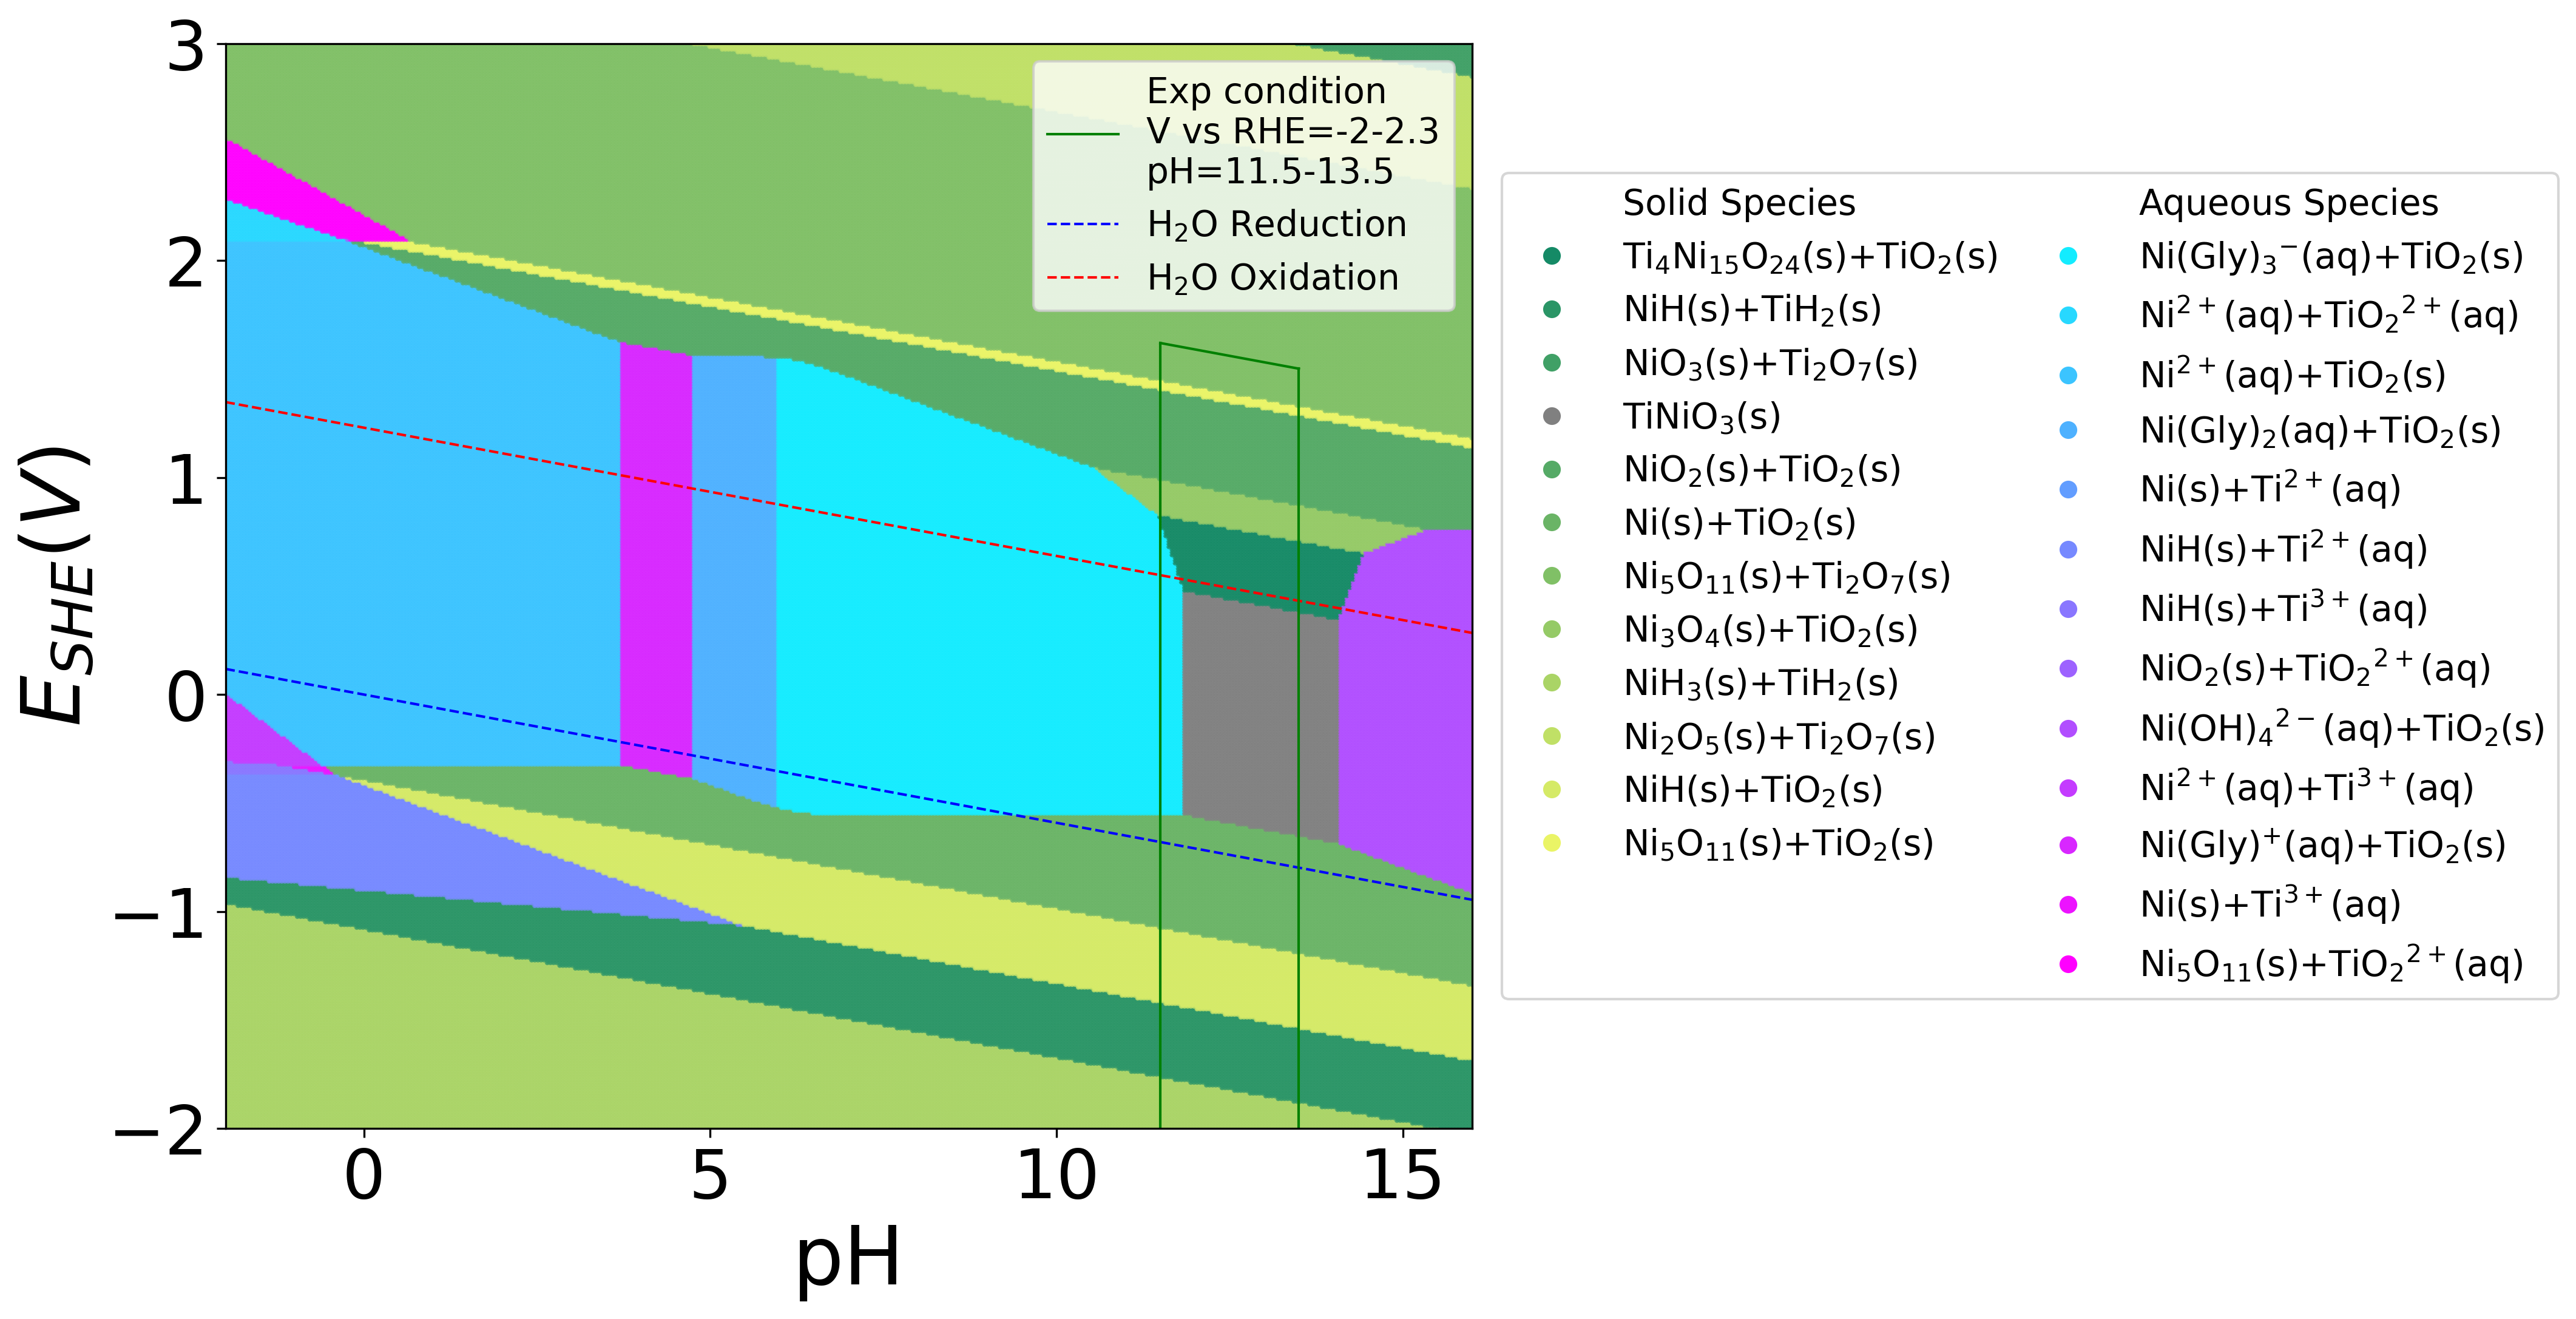
\includegraphics[width=\textwidth]
        {Figures/alloy_pourbaix_diagrams/Ti_Ni_alloy_Ti0.5 Ni0.5_NH3=0.02M_Gly=0.005M_CN=0M_activity=1e-04M.png}
        \par\medskip
    \end{subfigure}
    \begin{subfigure}[b]{0.45\textwidth}
        \subcaption{}\label{fig:TiNi_Pourbaix_NH3_Gly_CN}
        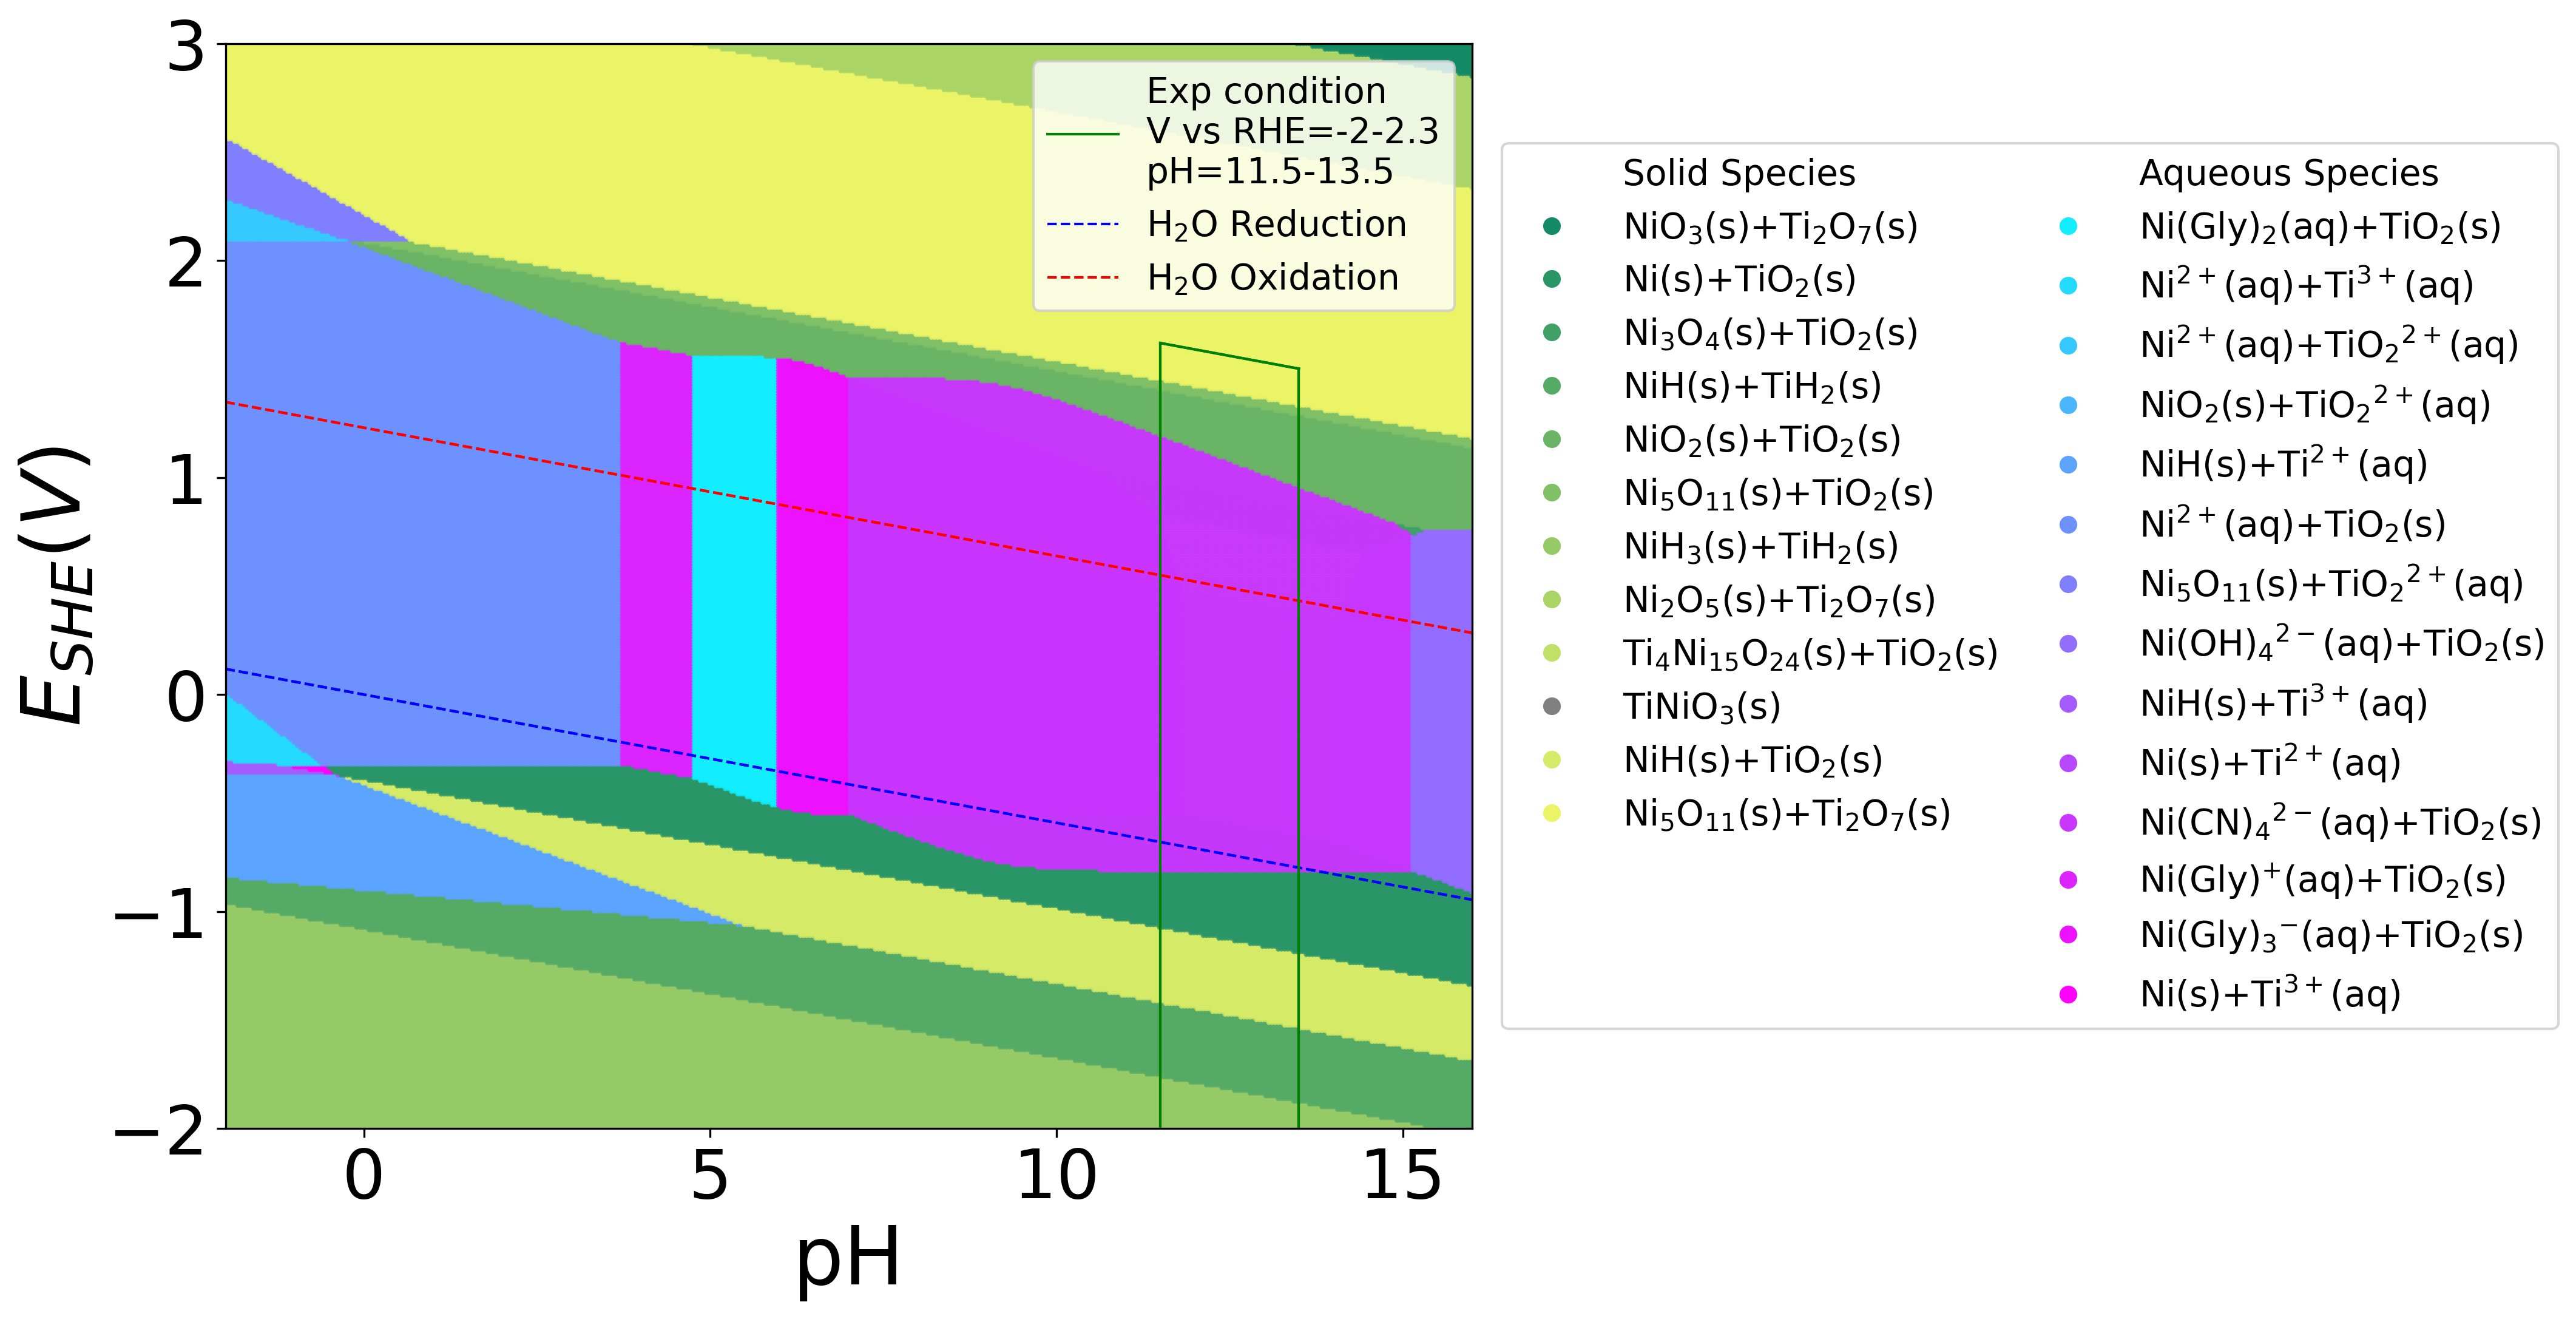
\includegraphics[width=\textwidth]{Figures/alloy_pourbaix_diagrams/Ti_Ni_alloy_Ti0.5 Ni0.5_NH3=0.02M_Gly=0.005M_CN=0.0001M_activity=1e-04M.png}
        \par\medskip   
    \end{subfigure}
    \caption{TiNi alloy Pourbaix diagrams with $\text{ion activity} = \num{1e-4}$: (a) $[\ce{NH3}]_\text{initial} = 0.02$~M, $[\text{Gly}]_\text{initial} = 0.005$~M; (b) $[\ce{NH3}]_\text{initial} = 0.02$~M, $[\text{Gly}]_\text{initial} = 0.005$~M, and $[\ce{CN^-}]_\text{initial} = \num{1e-4}$~M. A fixed reference stoichiometry of Ti:Ni = 1:1 was applied as a compositional constraint when generating the alloy Pourbaix diagrams. The green box highlights the experimentally relevant region, defined by an applied potential of \SIrange{-2}{2}{V} vs. RHE and a pH range of 11.5 to 13.5. Thermodynamically stable alloy regions are shaded in grey.}
    \label{fig:TiNi_alloy_Pourbaix}
\end{figure}

%%%%%%%%%%%%%%%%%%%%%%%%%%%%%%%%% TiCu Alloy %%%%%%%%%%%%%%%%%%%%%%%%%%%%%%%%%
\begin{figure}[htbp]
    \centering
    \begin{subfigure}[b]{0.45\textwidth}
        \subcaption{}\label{fig:TiCu_Pourbaix_NH3_Gly}
        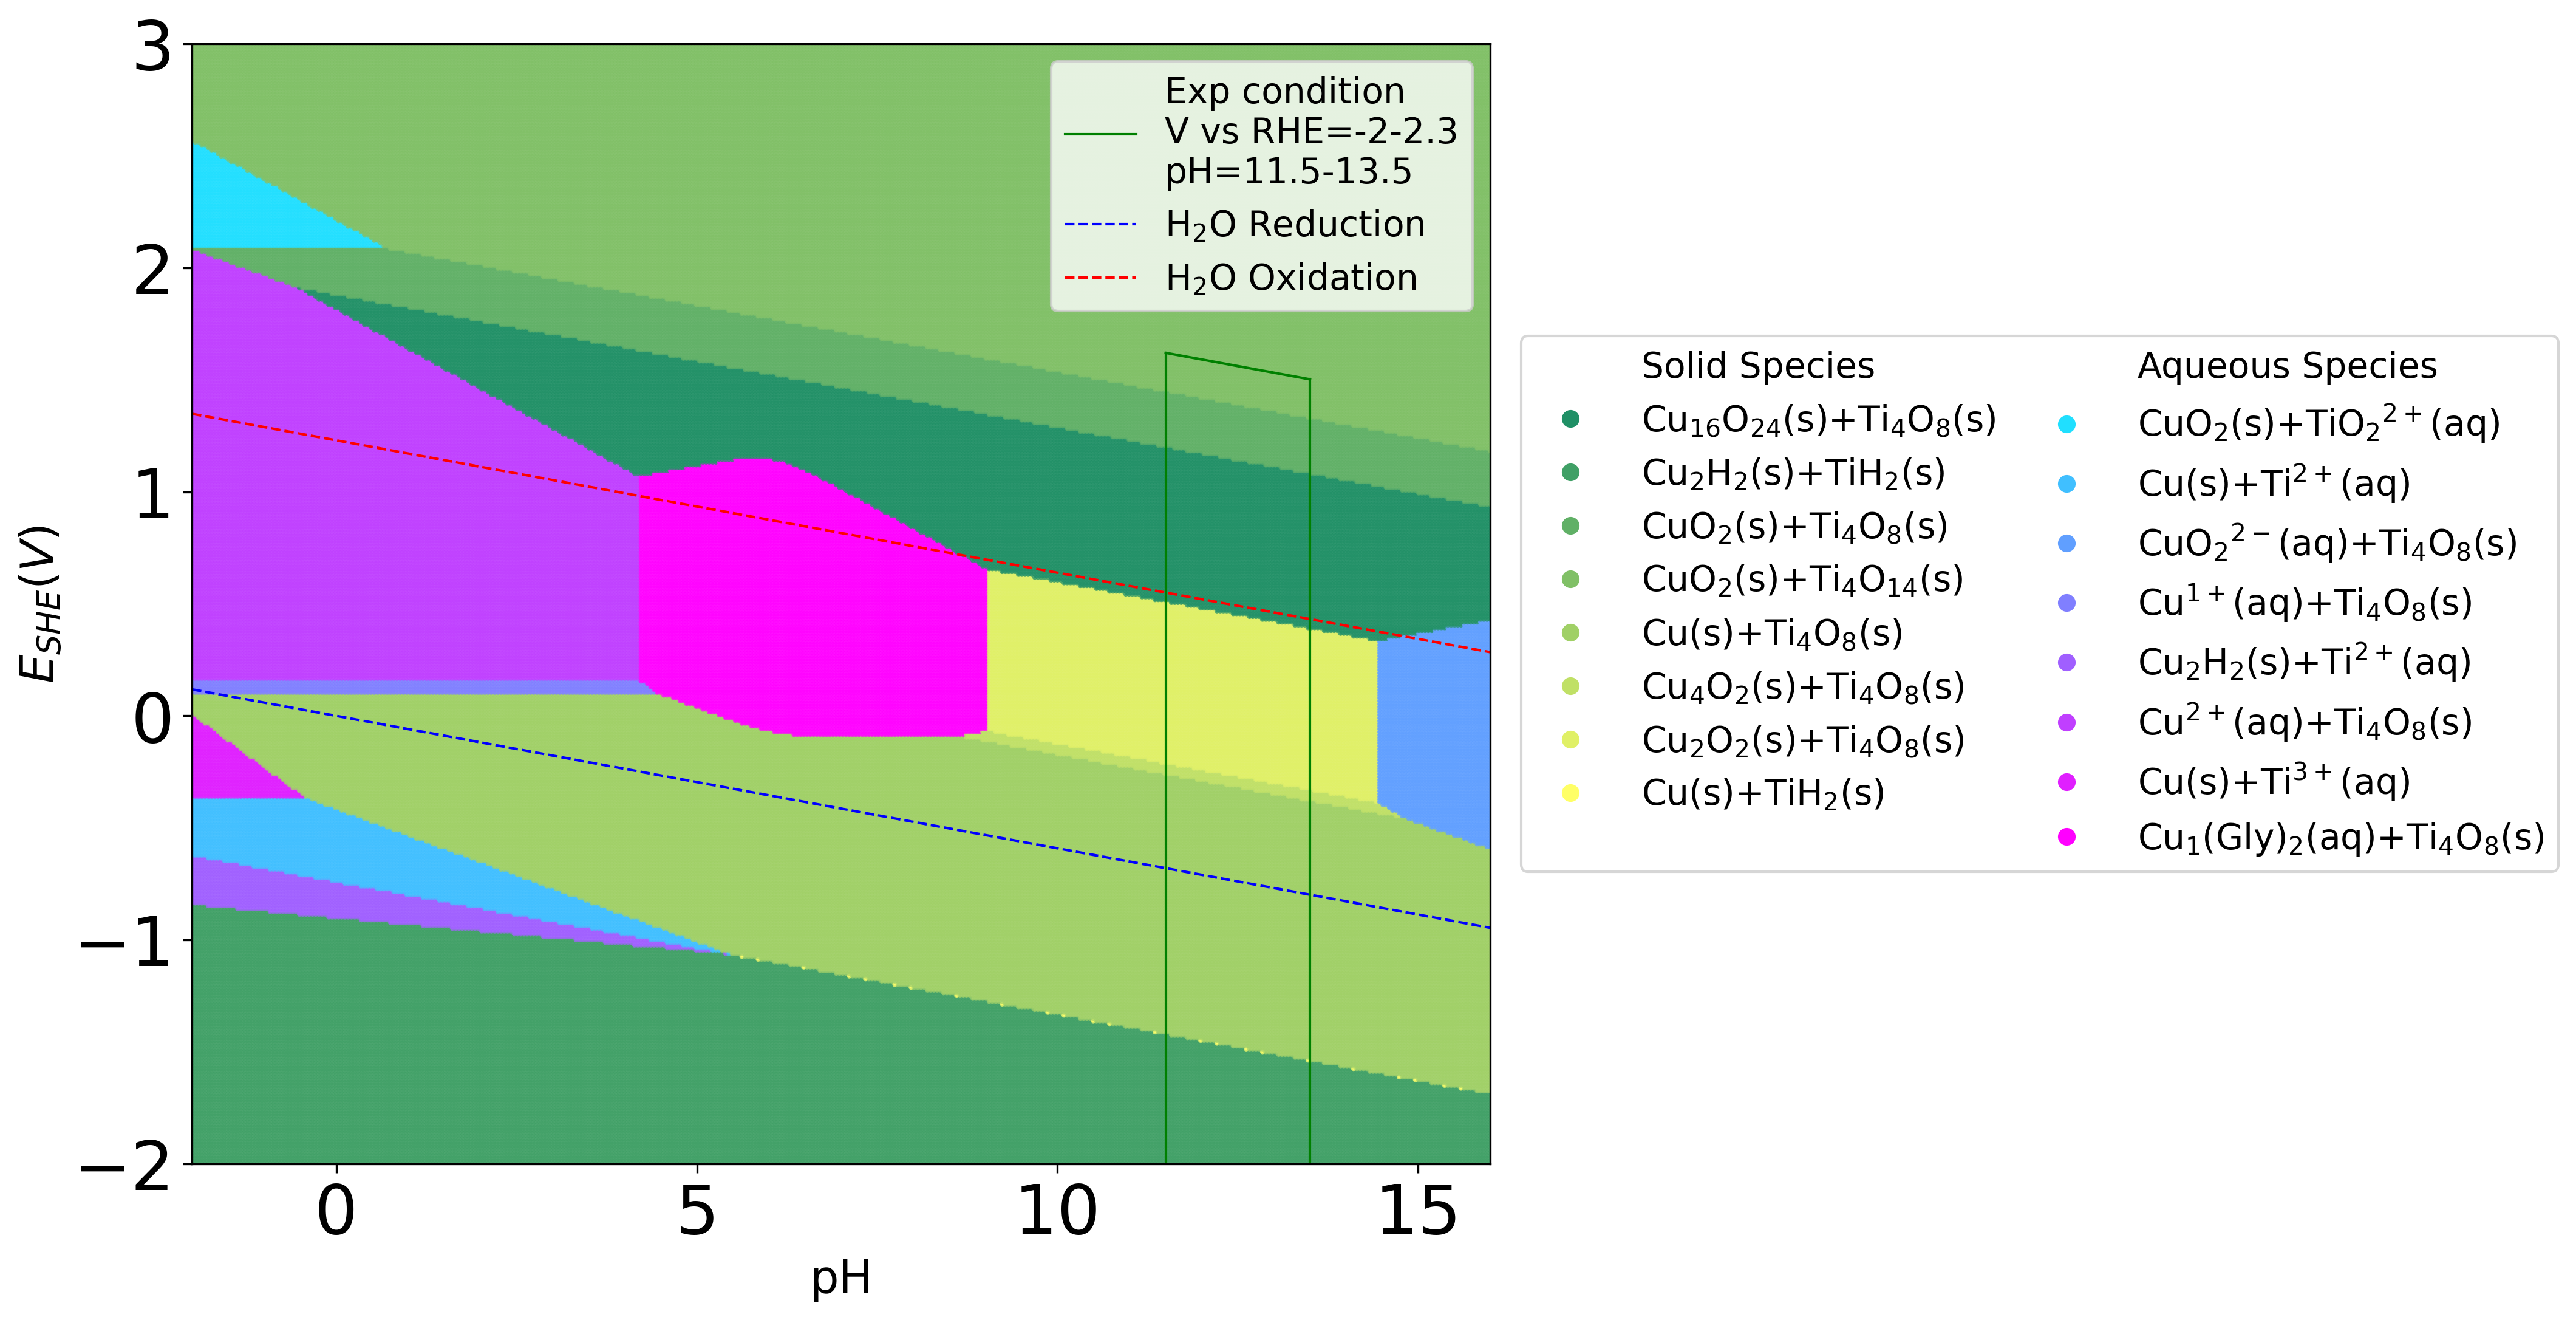
\includegraphics[width=\textwidth]
        {Figures/alloy_pourbaix_diagrams/Ti_Cu_alloy_Ti0.5 Cu0.5_NH3=0.02M_Gly=0.005M_CN=0M_activity=1e-04M.png}
        \par\medskip
    \end{subfigure}
    \begin{subfigure}[b]{0.45\textwidth}
        \subcaption{}\label{fig:TiCu_Pourbaix_NH3_Gly_CN}
        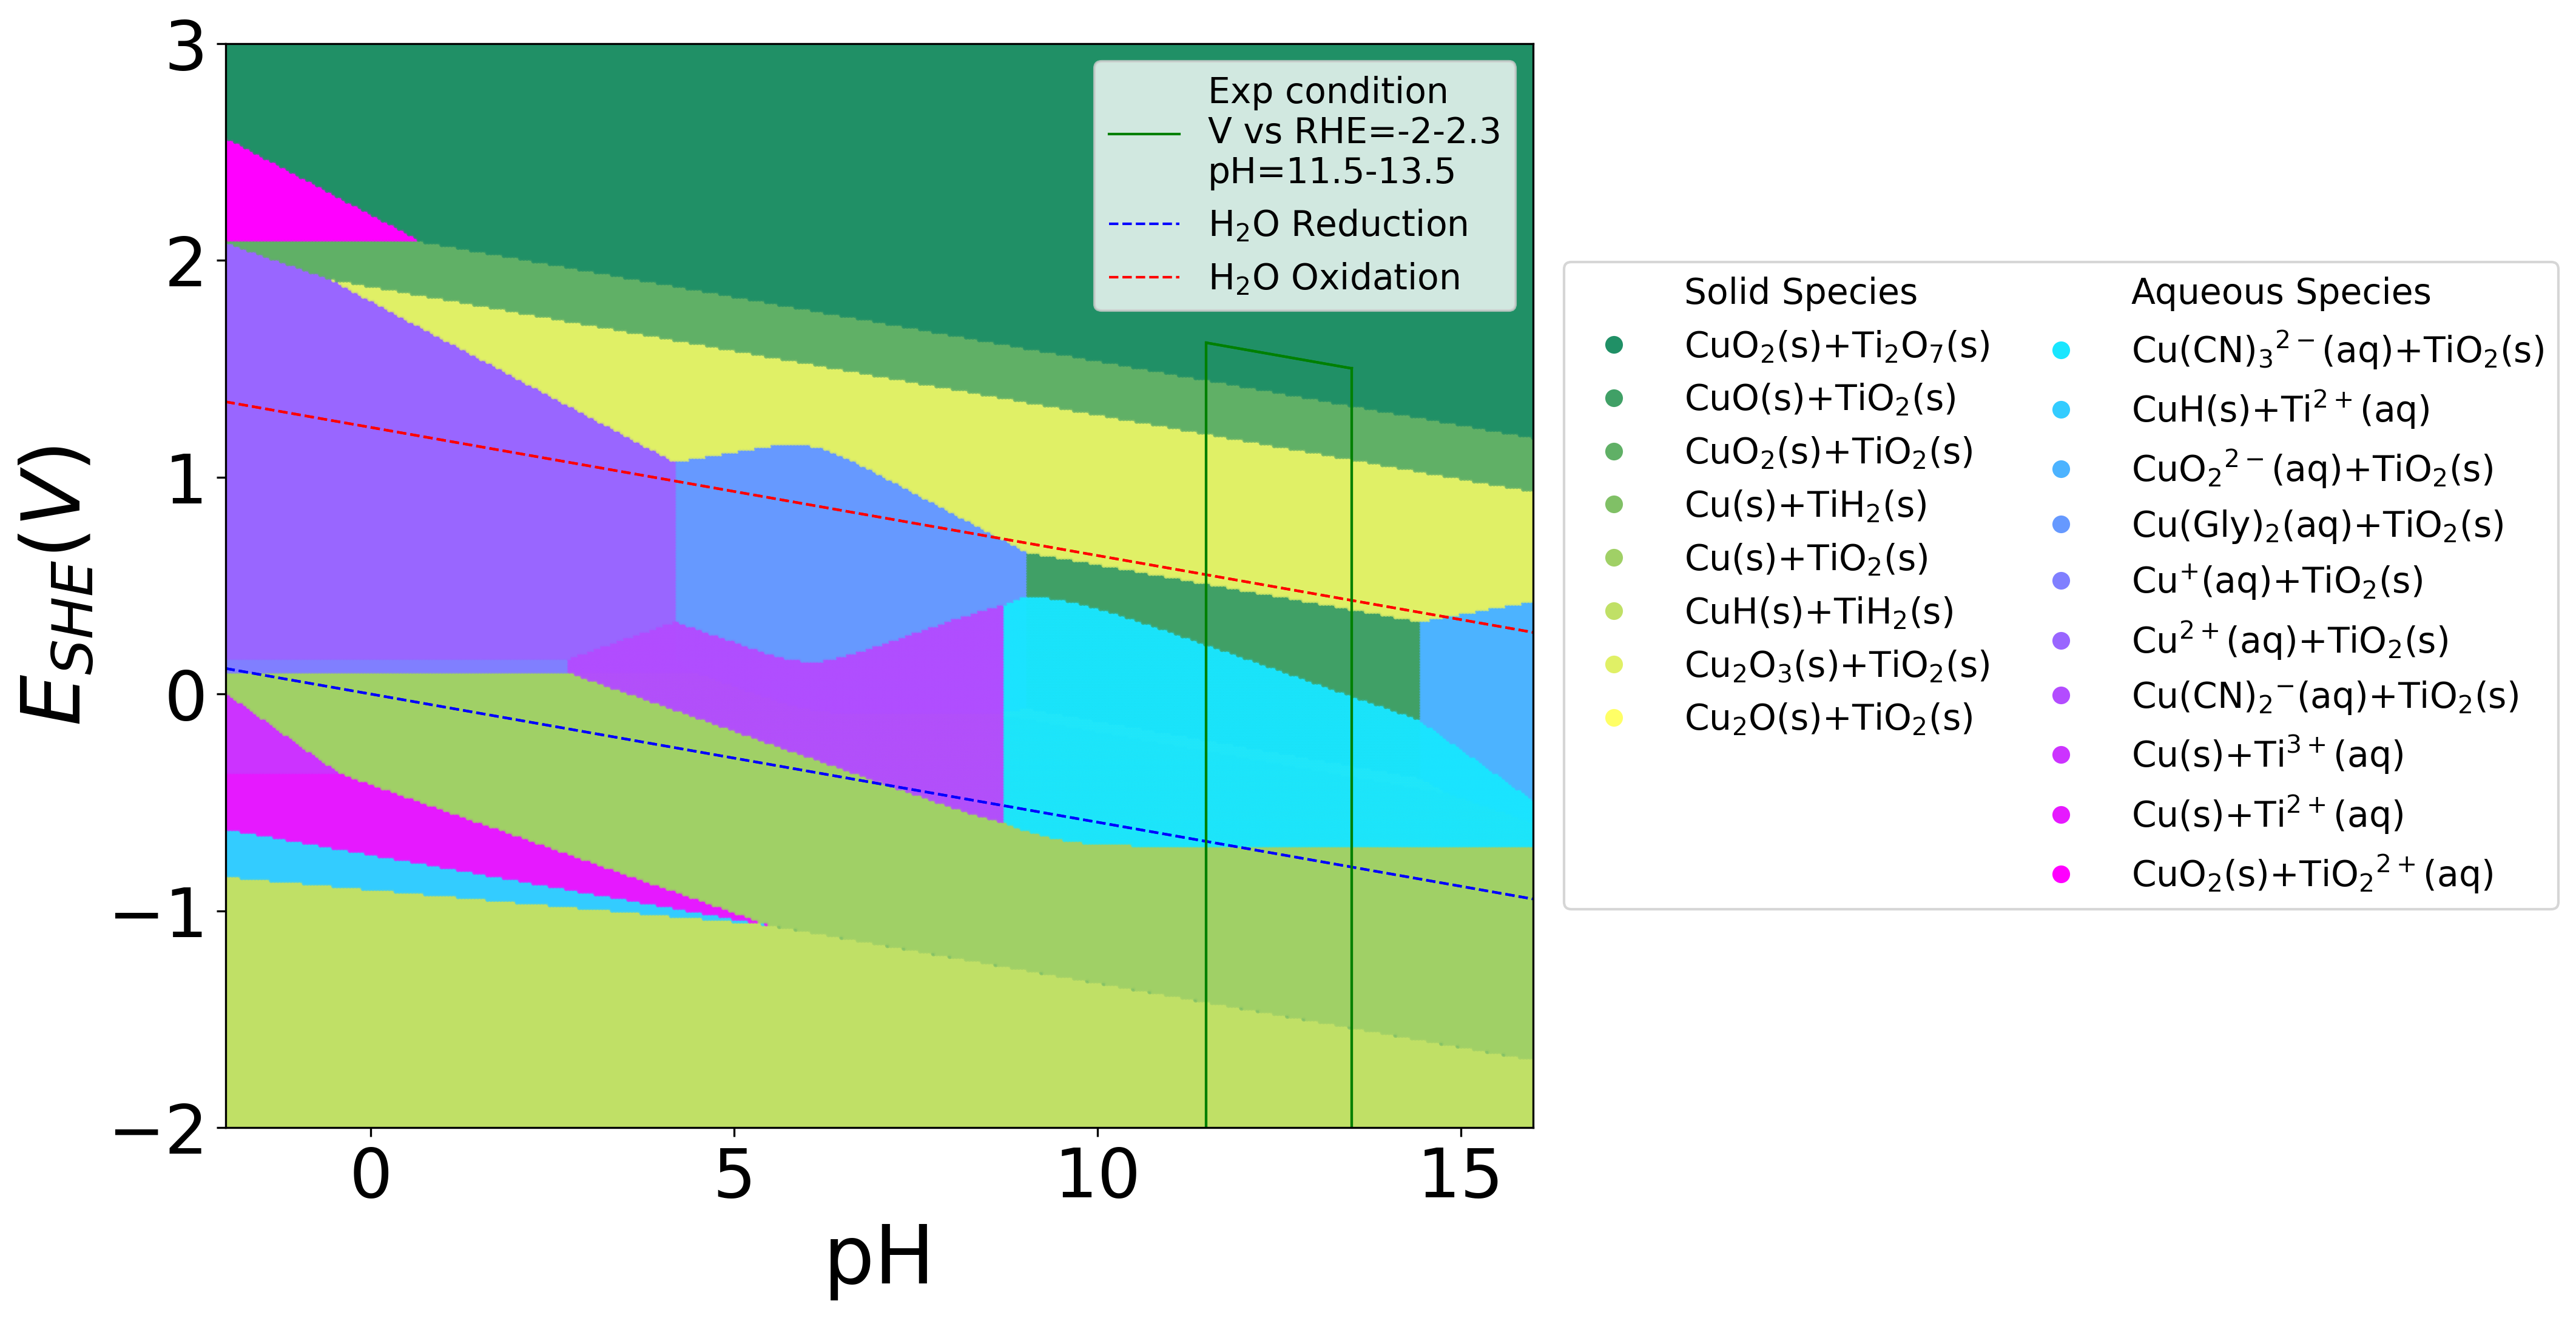
\includegraphics[width=\textwidth]{Figures/alloy_pourbaix_diagrams/Ti_Cu_alloy_Ti0.5 Cu0.5_NH3=0.02M_Gly=0.005M_CN=0.0001M_activity=1e-04M.png}
        \par\medskip   
    \end{subfigure}
    \caption{TiCu alloy Pourbaix diagrams with $\text{ion activity} = \num{1e-4}$: (a) $[\ce{NH3}]_\text{initial} = 0.02$~M, $[\text{Gly}]_\text{initial} = 0.005$~M; (b) $[\ce{NH3}]_\text{initial} = 0.02$~M, $[\text{Gly}]_\text{initial} = 0.005$~M, and $[\ce{CN^-}]_\text{initial} = \num{1e-4}$~M. A fixed reference stoichiometry of Ti:Cu = 1:1 was applied as a compositional constraint when generating the alloy Pourbaix diagrams. The green box highlights the experimentally relevant region, defined by an applied potential of \SIrange{-2}{2}{V} vs. RHE and a pH range of 11.5 to 13.5. Thermodynamically stable alloy regions are shaded in grey.}
    \label{fig:TiCu_alloy_Pourbaix}
\end{figure}

%%%%%%%%%%%%%%%%%%%%%%%%%%%%%%%%% PdAu Alloy %%%%%%%%%%%%%%%%%%%%%%%%%%%%%%%%%
\begin{figure}[htbp]
    \centering
    \begin{subfigure}[b]{0.45\textwidth}
        \subcaption{}\label{fig:PdAu_Pourbaix_NH3_Gly}
        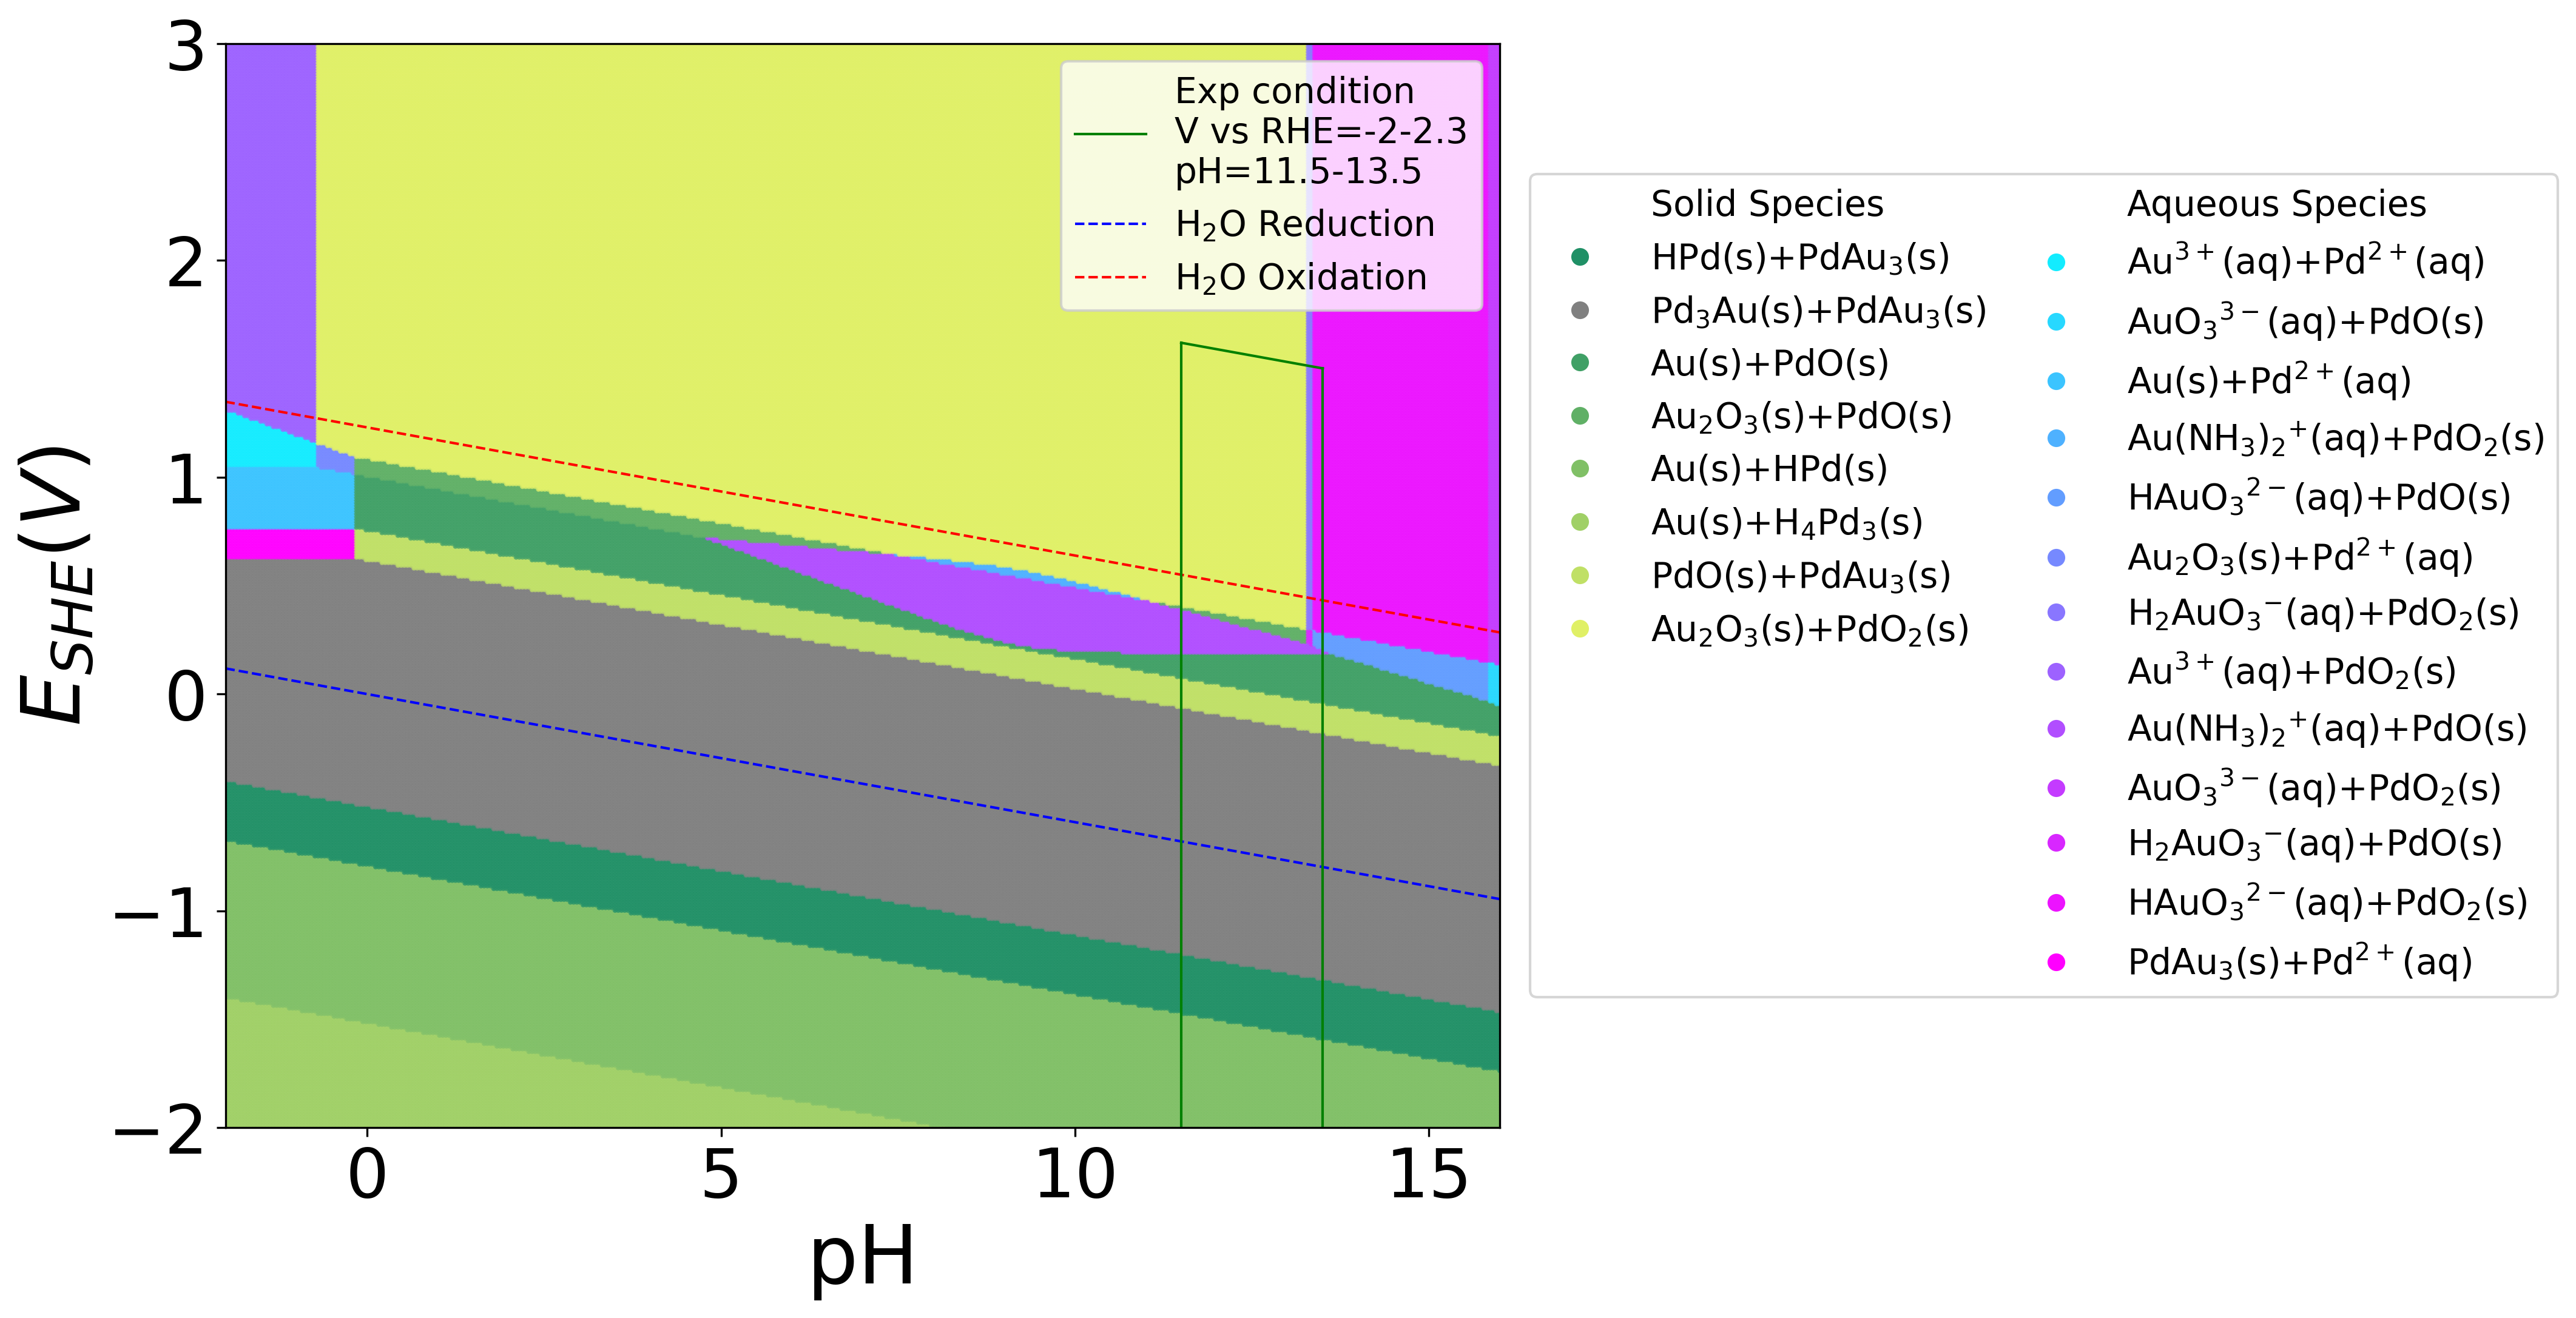
\includegraphics[width=\textwidth]
        {Figures/alloy_pourbaix_diagrams/Pd_Au_alloy_Pd0.5 Au0.5_NH3=0.02M_Gly=0.005M_CN=0M_activity=1e-04M.png}
        \par\medskip
    \end{subfigure}
    \begin{subfigure}[b]{0.45\textwidth}
        \subcaption{}\label{fig:PdAu_Pourbaix_NH3_Gly_CN}
        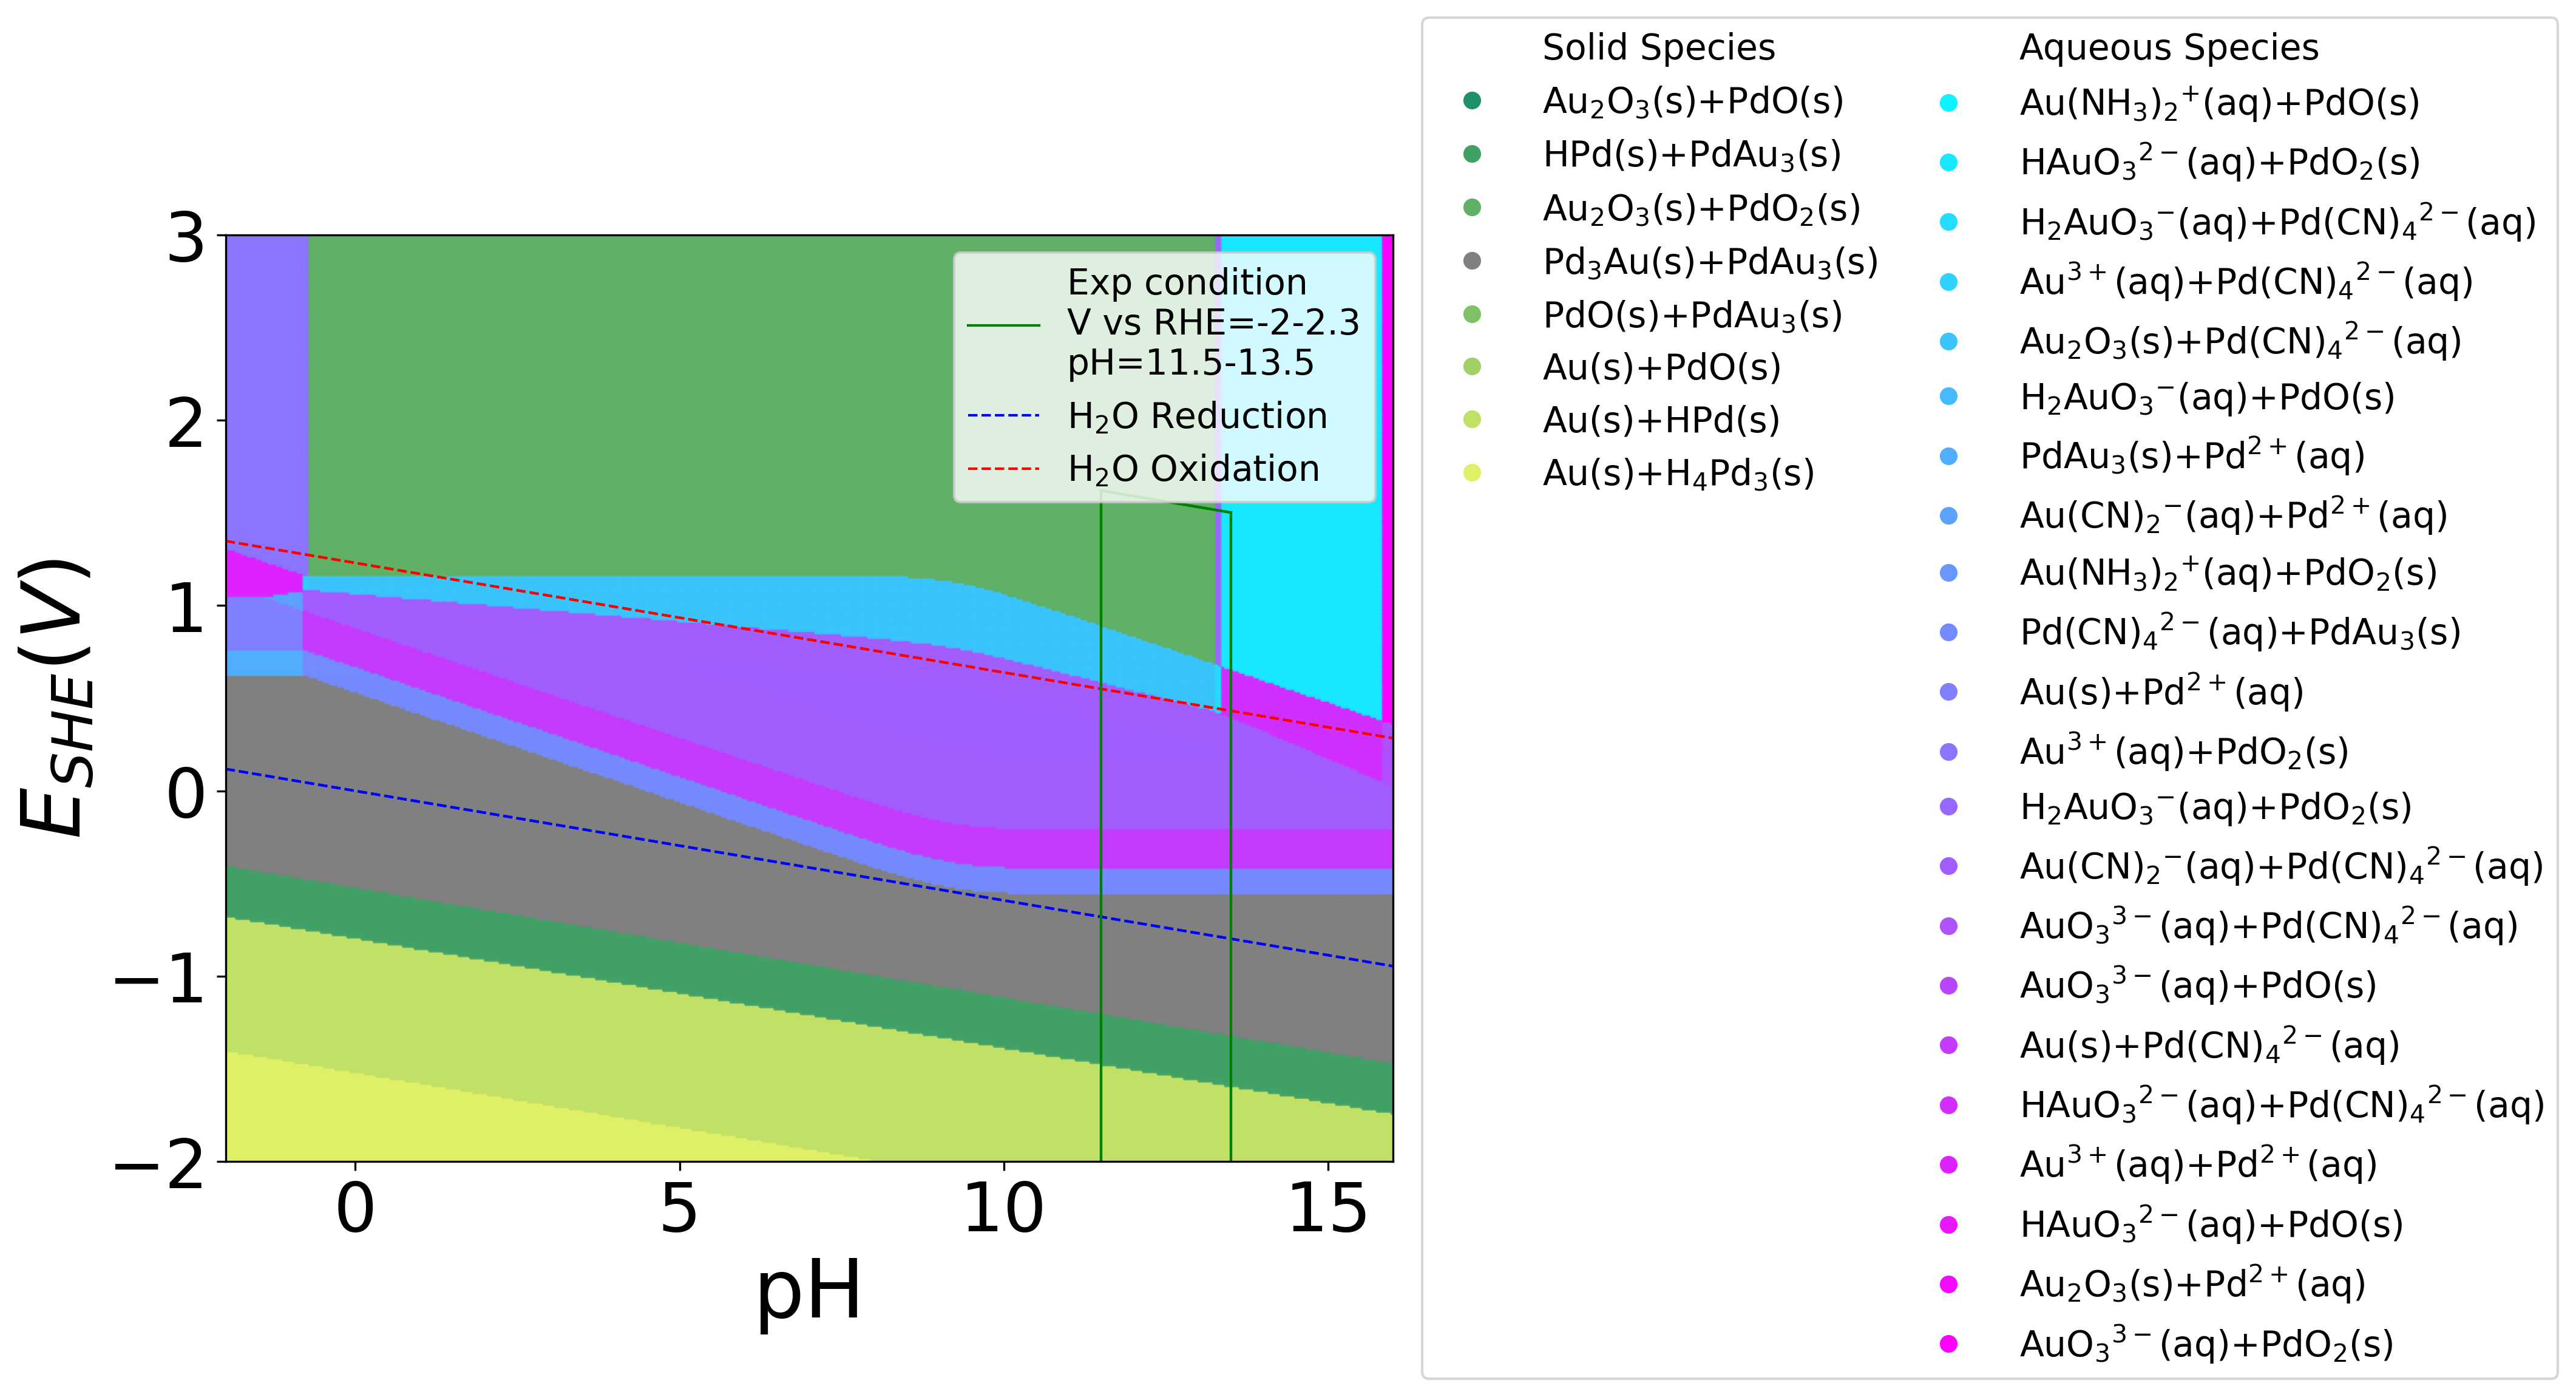
\includegraphics[width=\textwidth]{Figures/alloy_pourbaix_diagrams/Pd_Au_alloy_Pd0.5 Au0.5_NH3=0.02M_Gly=0.005M_CN=0.0001M_activity=1e-04M.png}
        \par\medskip   
    \end{subfigure}
    \caption{PdAu alloy Pourbaix diagrams with $\text{ion activity} = \num{1e-4}$: (a) $[\ce{NH3}]_\text{initial} = 0.02$~M, $[\text{Gly}]_\text{initial} = 0.005$~M; (b) $[\ce{NH3}]_\text{initial} = 0.02$~M, $[\text{Gly}]_\text{initial} = 0.005$~M, and $[\ce{CN^-}]_\text{initial} = \num{1e-4}$~M. A fixed reference stoichiometry of Pd:Au = 1:1 was applied as a compositional constraint when generating the alloy Pourbaix diagrams. The green box highlights the experimentally relevant region, defined by an applied potential of \SIrange{-2}{2}{V} vs. RHE and a pH range of 11.5 to 13.5. Thermodynamically stable alloy regions are shaded in grey.}
    \label{fig:PdAu_alloy_Pourbaix}
\end{figure}



\section{Conclusion}
% This study evaluates the stability of Ni, Cu, Pd, Pt, and Ti electrodes under EWAS conditions using Pourbaix diagrams, revealing the significant influence of nitrogen-containing ligands on metal corrosion behavior. While Ni and Cu exhibit strong resistance in aqueous environments, they become highly susceptible to dissolution in the presence of \ce{CN^-} ligands, necessitating careful solution composition control to prevent electrode degradation and contamination. Pd and Pt remain largely unaffected by glycine and ammonia but are vulnerable to cyanide complexation, with uncertainties in reported stability constants further complicating their viability. Given their high cost and instability in cyanide-rich environments, Pd and Pt are not ideal for EWAS applications. In contrast, Ti maintains excellent corrosion resistance due to its passivating oxide layer, making it the most promising candidate despite its low electronic conductivity, which can be addressed through conductive Ti-based materials. These findings highlight the importance of integrating stability considerations into electrode design, ensuring durability and minimizing contamination risks in electrochemical nutrient recovery systems.

This study evaluates the stability of Ni, Cu, Pd, Pt, and Ti electrodes EWASconditions using Pourbaix diagrams, highlighting the critical role of nitrogen-containing ligands in governing corrosion behavior. While Ni and Cu exhibit strong resistance to oxidation in pure aqueous environments, they are highly susceptible to dissolution in the presence of \ce{CN^-} ligands, underscoring the importance of controlling solution composition to mitigate electrode degradation and metal leaching. Pd and Pt are relatively inert toward glycine and ammonia but form stable cyanide complexes even at low concentrations, with inconsistencies in reported stability constants introducing uncertainty in their predicted durability. Given these limitations, alongside their high cost, Pd and Pt are less favorable candidates for EWAS deployment.

In contrast, Ti demonstrates excellent corrosion resistance across the EWAS-relevant pH and potential range due to its robust passivating oxide layer. However, its poor electronic conductivity may limit catalytic performance unless incorporated into conductive architectures such as doped perovskites, MXenes, or metal alloys.

To address this, we explored the stability of Ti-based and Pd-based alloys using Pourbaix diagrams. Alloys such as TiNi and TiCu combine the corrosion resistance of Ti with the catalytic activity or conductivity of the dopant metal, offering a pathway toward functionally optimized electrode materials. Additionally, PdAu alloys are investigated for their potential to improve the balance between catalytic activity and stability under redox-dynamic EWAS conditions. These alloying strategies demonstrate that tailored compositions can mitigate the trade-offs between stability, activity, and conductivity, making them promising candidates for durable and efficient nutrient recovery systems.

Overall, this work emphasizes the importance of integrating thermodynamic screening of both pure and alloyed materials to guide the rational design of EWAS electrodes with enhanced corrosion resistance, minimal leaching, and sustained performance in nitrogen-rich, alkaline environments.




\section{CRediT authorship contribution statement}
Nianhan Tian: Conceptualization, Methodology, Formal analysis, Software, Visualization, Writing – Original Draft.  
Ehsan Abbasi: Investigation, Validation, Writing – Review \& Editing.  
Haldrian Iriawan: Investigation, Validation, Writing – Review \& Editing.  
Paul Kohl: Resources, Writing – Review \& Editing.  
Andrew J. Medford: Conceptualization, Supervision, Project administration, Writing – Review \& Editing.


% Pourbaix diagrams of metal-\ce{NH3}/glycine/\ce{CN-}-\ce{H2O} are generated and discussed to identify thermodynamic behavior of an ideal material what can be used as an electrode in EWAS. The dissolvation behavior of various electrode under oxidizing potentials and high N-ligand concentrations was well explained by these pourbaix diagrams. The stability regions of build Ti and it oxides compared with other metals present its thermodynamically stability under such conditions. 
% \subsection{Outline}



\begin{acknowledgement}

% Please use ``The authors thank \ldots'' rather than ``The
% authors would like to thank \ldots''.

% The author thanks Mats Dahlgren for version one of \textsf{achemso},
% and Donald Arseneau for the code taken from \textsf{cite} to move
% citations after punctuation. Many users have provided feedback on the
% class, which is reflected in all of the different demonstrations
% shown in this document.

\end{acknowledgement}

%%%%%%%%%%%%%%%%%%%%%%%%%%%%%%%%%%%%%%%%%%%%%%%%%%%%%%%%%%%%%%%%%%%%%
%% The same is true for Supporting Information, which should use the
%% suppinfo environment.
%%%%%%%%%%%%%%%%%%%%%%%%%%%%%%%%%%%%%%%%%%%%%%%%%%%%%%%%%%%%%%%%%%%%%
\begin{suppinfo}
Free energies of metal-ligand complexes are available.


\end{suppinfo}
% \documentclass[journal=jacsat,manuscript=article,email=false]{achemso}

\usepackage[version=4]{mhchem} % Formula subscripts using \ce{}
\usepackage{esint}
\usepackage{threeparttable}
\usepackage{xr-hyper} % hyperlinks
\usepackage{hyperref} % hyperlinks
\usepackage{cleveref}
\usepackage{fancyhdr}
\usepackage[numbers]{natbib}
% To number sections, pages, figures and tables nested within chapters:
% \renewcommand{\thepage}{\arabic{chapter}.\arabic{page}} 
% \renewcommand{\thesection}{\arabic{chapter}.\arabic{section}}  
% \renewcommand{\thetable}{\arabic{chapter}.\arabic{table}}  
% \renewcommand{\thefigure}{\arabic{chapter}.\arabic{figure}}

% To number supplemental material with 'S':
% \renewcommand{\thepage}{S\arabic{page}} 
\renewcommand{\thesection}{S\arabic{section}}  
\renewcommand{\thetable}{S\arabic{table}}  
\renewcommand{\thefigure}{S\arabic{figure}}
\renewcommand{\theequation}{S\arabic{equation}}

\usepackage{longtable} % For multi-page tables
\usepackage{array}

\pagestyle{fancy}
\fancyhf{}
\cfoot{S\thepage}
\renewcommand{\headrulewidth}{0pt}


\author{Nianhan Tian}
\affiliation[Georgia Institute of Technology]
{School of Chemical and Biomolecular Engineering, Georgia Institute of Technology, Atlanta, Georgia 30318 USA}

\author{Andrew J. Medford}
\affiliation[Georgia Institute of Technology]
{School of Chemical and Biomolecular Engineering, Georgia Institute of Technology, Atlanta, Georgia 30318 USA}
\email{ajm@gatech.edu}

\title{Accelerated Computational Materials Discovery for Electrochemical Nutrient Recovery\\\vspace{8pt}\large{Supporting Information}}


\begin{document}
\newpage
\clearpage
\begin{longtable}{|p{4cm}|p{4cm}|p{3cm}|p{3cm}|}
\caption{Formation energies of species for \ce{NH3} complexes.} 
\label{tab:NH3_complex_energies}
\\
\hline
\textbf{Species} & \textbf{Metal ion} & \textbf{\( \Delta G^\circ_{298} \) (eV)} & \textbf{Reference} \\ \hline
\endfirsthead
\caption*{Table \thetable\ continued from previous pages.} \\
\hline
\textbf{Species} & \textbf{Metal ion} & \textbf{\( \Delta G^\circ_{298} \) (eV)} & \textbf{Reference} \\ \hline
\endhead
\hline
\endfoot
\hline
\endlastfoot
\ce{[Ag.0(NH3).0].0+} & \ce{Ag^1+} & 0.322 & \textnormal{\citenum{Bjerrum1957StabilitySubstances}} \\ \hline
\ce{[Ag.0(NH3)2.0].0+} & \ce{Ag^1+} & -0.191 & \textnormal{\citenum{Bjerrum1957StabilitySubstances}} \\ \hline
\ce{[Au.0(NH3)2.0].0+} & \ce{Au^1+} & -0.325 & \textnormal{\citenum{Bjerrum1957StabilitySubstances}} \\ \hline
\ce{[Au.0(NH3)4.0]^3.0+} & \ce{Au^3+} & 1.681 & \textnormal{\citenum{Bjerrum1957StabilitySubstances}} \\ \hline
\ce{[Ca.0(NH3).0]^2.0+} & \ce{Ca^2+} & -6.001 & \textnormal{\citenum{Bjerrum1957StabilitySubstances}} \\ \hline
\ce{[Ca.0(NH3)2.0]^2.0+} & \ce{Ca^2+} & -6.242 & \textnormal{\citenum{Bjerrum1957StabilitySubstances}} \\ \hline
\ce{[Ca.0(NH3)3.0]^2.0+} & \ce{Ca^2+} & -6.470 & \textnormal{\citenum{Bjerrum1957StabilitySubstances}} \\ \hline
\ce{[Ca.0(NH3)4.0]^2.0+} & \ce{Ca^2+} & -7.001 & \textnormal{\citenum{Bjerrum1957StabilitySubstances}} \\ \hline
\ce{[Cd.0(NH3).0]^2.0+} & \ce{Cd^2+} & -1.234 & \textnormal{\citenum{Bjerrum1957StabilitySubstances}} \\ \hline
\ce{[Cd.0(NH3)2.0]^2.0+} & \ce{Cd^2+} & -1.632 & \textnormal{\citenum{Bjerrum1957StabilitySubstances}} \\ \hline
\ce{[Cd.0(NH3)3.0]^2.0+} & \ce{Cd^2+} & -1.990 & \textnormal{\citenum{Bjerrum1957StabilitySubstances}} \\ \hline
\ce{[Cd.0(NH3)4.0]^2.0+} & \ce{Cd^2+} & -2.318 & \textnormal{\citenum{Bjerrum1957StabilitySubstances}} \\ \hline
\ce{[Cd.0(NH3)5.0]^2.0+} & \ce{Cd^2+} & -2.575 & \textnormal{\citenum{Bjerrum1957StabilitySubstances}} \\ \hline
\ce{[Cd.0(NH3)6.0]^2.0+} & \ce{Cd^2+} & -2.750 & \textnormal{\citenum{Bjerrum1957StabilitySubstances}} \\ \hline
\ce{[Co.0(NH3).0]^2.0+} & \ce{Co^2+} & -0.961 & \textnormal{\citenum{Bjerrum1957StabilitySubstances}} \\ \hline
\ce{[Co.0(NH3)2.0]^2.0+} & \ce{Co^2+} & -1.330 & \textnormal{\citenum{Bjerrum1957StabilitySubstances}} \\ \hline
\ce{[Co.0(NH3)3.0]^2.0+} & \ce{Co^2+} & -1.665 & \textnormal{\citenum{Bjerrum1957StabilitySubstances}} \\ \hline
\ce{[Co.0(NH3)4.0]^2.0+} & \ce{Co^2+} & -1.982 & \textnormal{\citenum{Bjerrum1957StabilitySubstances}} \\ \hline
\ce{[Co.0(NH3)5.0]^2.0+} & \ce{Co^2+} & -2.260 & \textnormal{\citenum{Bjerrum1957StabilitySubstances}} \\ \hline
\ce{[Co.0(NH3)6.0]^2.0+} & \ce{Co^2+} & -2.501 & \textnormal{\citenum{Bjerrum1957StabilitySubstances}} \\ \hline
\ce{[Co.0(NH3).0]^3.0+} & \ce{Co^3+} & 0.681 & \textnormal{\citenum{Bjerrum1957StabilitySubstances}} \\ \hline
\ce{[Co.0(NH3)2.0]^3.0+} & \ce{Co^3+} & 0.008 & \textnormal{\citenum{Bjerrum1957StabilitySubstances}} \\ \hline
\ce{[Co.0(NH3)3.0]^3.0+} & \ce{Co^3+} & -0.628 & \textnormal{\citenum{Bjerrum1957StabilitySubstances}} \\ \hline
\ce{[Co.0(NH3)4.0]^3.0+} & \ce{Co^3+} & -1.236 & \textnormal{\citenum{Bjerrum1957StabilitySubstances}} \\ \hline
\ce{[Co.0(NH3)5.0]^3.0+} & \ce{Co^3+} & -1.814 & \textnormal{\citenum{Bjerrum1957StabilitySubstances}} \\ \hline
\ce{[Co.0(NH3)6.0]^3.0+} & \ce{Co^3+} & -2.350 & \textnormal{\citenum{Bjerrum1957StabilitySubstances}} \\ \hline
\ce{[Cu.0(NH3).0].0+} & \ce{Cu^1+} & -0.107 & \textnormal{\citenum{Bjerrum1957StabilitySubstances}} \\ \hline
\ce{[Cu.0(NH3)2.0].0+} & \ce{Cu^1+} & -0.673 & \textnormal{\citenum{Bjerrum1957StabilitySubstances}} \\ \hline
\ce{[Cu.0(NH3).0]^2.0+} & \ce{Cu^2+} & 0.158 & \textnormal{\citenum{Bjerrum1957StabilitySubstances}} \\ \hline
\ce{[Cu.0(NH3)2.0]^2.0+} & \ce{Cu^2+} & -0.324 & \textnormal{\citenum{Bjerrum1957StabilitySubstances}} \\ \hline
\ce{[Cu.0(NH3)3.0]^2.0+} & \ce{Cu^2+} & -0.769 & \textnormal{\citenum{Bjerrum1957StabilitySubstances}} \\ \hline
\ce{[Cu.0(NH3)4.0]^2.0+} & \ce{Cu^2+} & -1.170 & \textnormal{\citenum{Bjerrum1957StabilitySubstances}} \\ \hline
\ce{[Fe.0(NH3).0]^2.0+} & \ce{Fe^2+} & -1.177 & \textnormal{\citenum{Bjerrum1957StabilitySubstances}} \\ \hline
\ce{[Fe.0(NH3)2.0]^2.0+} & \ce{Fe^2+} & -1.500 & \textnormal{\citenum{Bjerrum1957StabilitySubstances}} \\ \hline
\ce{[Fe.0(NH3)4.0]^2.0+} & \ce{Fe^2+} & -2.141 & \textnormal{\citenum{Bjerrum1957StabilitySubstances}} \\ \hline
\ce{[Ni.0(NH3).0]^2.0+} & \ce{Ni^2+} & -0.920 & \textnormal{\citenum{Bjerrum1957StabilitySubstances}} \\ \hline
\ce{[Ni.0(NH3)2.0]^2.0+} & \ce{Ni^2+} & -1.326 & \textnormal{\citenum{Bjerrum1957StabilitySubstances}} \\ \hline
\ce{[Ni.0(NH3)3.0]^2.0+} & \ce{Ni^2+} & -1.702 & \textnormal{\citenum{Bjerrum1957StabilitySubstances}} \\ \hline
\ce{[Ni.0(NH3)4.0]^2.0+} & \ce{Ni^2+} & -2.046 & \textnormal{\citenum{Bjerrum1957StabilitySubstances}} \\ \hline
\ce{[Ni.0(NH3)5.0]^2.0+} & \ce{Ni^2+} & -2.364 & \textnormal{\citenum{Bjerrum1957StabilitySubstances}} \\ \hline
\ce{[Ni.0(NH3)6.0]^2.0+} & \ce{Ni^2+} & -2.639 & \textnormal{\citenum{Bjerrum1957StabilitySubstances}} \\ \hline
\ce{[Mg.0(NH3).0]^2.0+} & \ce{Mg^2+} & -5.003 & \textnormal{\citenum{Bjerrum1957StabilitySubstances}} \\ \hline
\ce{[Mg.0(NH3)2.0]^2.0+} & \ce{Mg^2+} & -5.270 & \textnormal{\citenum{Bjerrum1957StabilitySubstances}} \\ \hline
\ce{[Mg.0(NH3)3.0]^2.0+} & \ce{Mg^2+} & -5.520 & \textnormal{\citenum{Bjerrum1957StabilitySubstances}} \\ \hline
\ce{[Mg.0(NH3)4.0]^2.0+} & \ce{Mg^2+} & -5.753 & \textnormal{\citenum{Bjerrum1957StabilitySubstances}} \\ \hline
\ce{[Mn.0(NH3).0]^2.0+} & \ce{Mn^2+} & -2.687 & \textnormal{\citenum{Bjerrum1957StabilitySubstances}} \\ \hline
\ce{[Mn.0(NH3)2.0]^2.0+} & \ce{Mn^2+} & -2.993 & \textnormal{\citenum{Bjerrum1957StabilitySubstances}} \\ \hline
\ce{[Zn.0(NH3).0]^2.0+} & \ce{Zn^2+} & -1.934 & \textnormal{\citenum{Bjerrum1957StabilitySubstances}} \\ \hline
\ce{[Zn.0(NH3)2.0]^2.0+} & \ce{Zn^2+} & -2.349 & \textnormal{\citenum{Bjerrum1957StabilitySubstances}} \\ \hline
\ce{[Zn.0(NH3)3.0]^2.0+} & \ce{Zn^2+} & -2.767 & \textnormal{\citenum{Bjerrum1957StabilitySubstances}} \\ \hline
\ce{[Zn.0(NH3)4.0]^2.0+} & \ce{Zn^2+} & -3.164 & \textnormal{\citenum{Bjerrum1957StabilitySubstances}} \\ \hline
\ce{[Pt.0(NH3)4.0]^2.0+} & \ce{Pt^2+} & -0.552 & \textnormal{\citenum{Sillen1964StabilityComplexes}} \\ \hline
\ce{[Pd.0(NH3).0]^2.0+} & \ce{Pd^2+} & 0.985 & \textnormal{\citenum{Smith1989CriticalConstants}} \\ \hline
\ce{[Pd.0(NH3)2.0]^2.0+} & \ce{Pd^2+} & 0.183 & \textnormal{\citenum{Smith1989CriticalConstants}} \\ \hline
\ce{[Pd.0(NH3)3.0]^2.0+} & \ce{Pd^2+} & -0.537 & \textnormal{\citenum{Smith1989CriticalConstants}} \\ \hline
\ce{[Pd.0(NH3)4.0]^2.0+} & \ce{Pd^2+} & -1.215 & \textnormal{\citenum{Smith1989CriticalConstants}} \\ \hline
\ce{[Zr.0(NH3).0].0+} & \ce{Zr^1+} & 3.127 & \textnormal{\citenum{Aviles2022ExploringNH3}} \\ \hline
\ce{[Zr.0(NH3)2.0].0+} & \ce{Zr^1+} & 3.248 & \textnormal{\citenum{Aviles2022ExploringNH3}} \\ \hline
\ce{[Zr.0(NH3)3.0].0+} & \ce{Zr^1+} & 2.498 & \textnormal{\citenum{Aviles2022ExploringNH3}} \\ \hline
\ce{[Zr.0(NH3)4.0].0+} & \ce{Zr^1+} & 2.450 & \textnormal{\citenum{Aviles2022ExploringNH3}} \\ \hline
\ce{[Zr.0(NH3)5.0].0+} & \ce{Zr^1+} & 2.042 & \textnormal{\citenum{Aviles2022ExploringNH3}} \\ \hline
\ce{[Zr.0(NH3)6.0].0+} & \ce{Zr^1+} & 2.307 & \textnormal{\citenum{Aviles2022ExploringNH3}} \\ \hline
\ce{[Zr.0(NH3)7.0].0+} & \ce{Zr^1+} & 1.930 & \textnormal{\citenum{Aviles2022ExploringNH3}}\end{longtable}

\newpage
\clearpage
\begin{longtable}{|p{4cm}|p{4cm}|p{3cm}|p{3cm}|}
\caption{Formation energies of species for \ce{Gly-} complexes.} 
\label{tab:Gly[1-]_complex_energies}
\\
\hline
\textbf{Species} & \textbf{Metal ion} & \textbf{\( \Delta G^\circ_{298} \) (eV)} & \textbf{Reference} \\ \hline
\endfirsthead
\caption*{Table \thetable\ continued from previous pages.} \\
\hline
\textbf{Species} & \textbf{Metal ion} & \textbf{\( \Delta G^\circ_{298} \) (eV)} & \textbf{Reference} \\ \hline
\endhead
\hline
\endfoot
\hline
\endlastfoot
\ce{[Au(Gly)2]-} & \ce{Au^1+} & -5.613 & \textnormal{\citenum{Azadi2019DataComplexes}} \\ \hline
\ce{[Au(Gly)]^2+} & \ce{Au^3+} & 0.880 & \textnormal{\citenum{Azadi2019DataComplexes}} \\ \hline
\ce{[Au(Gly)2]+} & \ce{Au^3+} & -2.591 & \textnormal{\citenum{Azadi2019DataComplexes}} \\ \hline
\ce{[Ag(Gly)]} & \ce{Ag^1+} & -3.046 & \textnormal{\citenum{Smith1989CriticalConstants}} \\ \hline
\ce{[Ag(Gly)2]-} & \ce{Ag^1+} & -6.458 & \textnormal{\citenum{Smith1989CriticalConstants}} \\ \hline
\ce{[Fe(Gly)]+} & \ce{Fe^2+} & -4.335 & \textnormal{\citenum{Smith1989CriticalConstants}} \\ \hline
\ce{[Fe(Gly)2]} & \ce{Fe^2+} & -7.805 & \textnormal{\citenum{Smith1989CriticalConstants}} \\ \hline
\ce{[Fe(Gly)]^2+} & \ce{Fe^3+} & -3.785 & \textnormal{\citenum{Smith1989CriticalConstants}} \\ \hline
\ce{[Cu(Gly)]} & \ce{Cu^1+} & -3.144 & \textnormal{\citenum{Smith1989CriticalConstants}} \\ \hline
\ce{[Cu(Gly)2]-} & \ce{Cu^1+} & -6.600 & \textnormal{\citenum{Smith1989CriticalConstants}} \\ \hline
\ce{[Cu(Gly)]+} & \ce{Cu^2+} & -3.064 & \textnormal{\citenum{Smith1989CriticalConstants}} \\ \hline
\ce{[Cu(Gly)2]} & \ce{Cu^2+} & -6.740 & \textnormal{\citenum{Smith1989CriticalConstants}} \\ \hline
\ce{[Cu(Gly)3]-} & \ce{Cu^2+} & -9.110 & \textnormal{\citenum{Smith1989CriticalConstants}} \\ \hline
\ce{[Mg(Gly)]+} & \ce{Mg^2+} & -8.180 & \textnormal{\citenum{Smith1989CriticalConstants}} \\ \hline
\ce{[Mg(Gly)2]} & \ce{Mg^2+} & -11.240 & \textnormal{\citenum{Smith1989CriticalConstants}} \\ \hline
\ce{[Mn(Gly)]+} & \ce{Mn^2+} & -5.816 & \textnormal{\citenum{Smith1989CriticalConstants}} \\ \hline
\ce{[Mn(Gly)2]} & \ce{Mn^2+} & -9.216 & \textnormal{\citenum{Smith1989CriticalConstants}} \\ \hline
\ce{[Mn(Gly)3]-} & \ce{Mn^2+} & -12.479 & \textnormal{\citenum{Smith1989CriticalConstants}} \\ \hline
\ce{[Ni(Gly)]+} & \ce{Ni^2+} & -4.087 & \textnormal{\citenum{Smith1989CriticalConstants}} \\ \hline
\ce{[Ni(Gly)2]} & \ce{Ni^2+} & -7.640 & \textnormal{\citenum{Smith1989CriticalConstants}} \\ \hline
\ce{[Ni(Gly)3]-} & \ce{Ni^2+} & -11.065 & \textnormal{\citenum{Smith1989CriticalConstants}} \\ \hline
\ce{[Zn(Gly)]+} & \ce{Zn^2+} & -5.114 & \textnormal{\citenum{Smith1989CriticalConstants}} \\ \hline
\ce{[Zn(Gly)2]} & \ce{Zn^2+} & -8.639 & \textnormal{\citenum{Smith1989CriticalConstants}} \\ \hline
\ce{[Zn(Gly)3]-} & \ce{Zn^2+} & -11.994 & \textnormal{\citenum{Smith1989CriticalConstants}} \\ \hline
\ce{[Co(Gly)]+} & \ce{Co^2+} & -4.105 & \textnormal{\citenum{Smith1989CriticalConstants}} \\ \hline
\ce{[Co(Gly)2]} & \ce{Co^2+} & -7.593 & \textnormal{\citenum{Smith1989CriticalConstants}} \\ \hline
\ce{[Co(Gly)3]-} & \ce{Co^2+} & -11.004 & \textnormal{\citenum{Smith1989CriticalConstants}} \\ \hline
\ce{[Cd(Gly)]+} & \ce{Cd^2+} & -4.312 & \textnormal{\citenum{Smith1989CriticalConstants}} \\ \hline
\ce{[Cd(Gly)2]} & \ce{Cd^2+} & -7.772 & \textnormal{\citenum{Smith1989CriticalConstants}} \\ \hline
\ce{[Cd(Gly)3]-} & \ce{Cd^2+} & -11.203 & \textnormal{\citenum{Azadi2019DataComplexes}} \\ \hline
\ce{[Na(Gly)]} & \ce{Na^1+} & -5.948 & \textnormal{\citenum{Azadi2019DataComplexes}} \\ \hline
\ce{[Ti(Gly)]} & \ce{Ti^1+} & -3.017 & \textnormal{\citenum{Azadi2019DataComplexes}} \\ \hline
\ce{[Ti(Gly)2]-} & \ce{Ti^1+} & -7.080 & \textnormal{\citenum{Azadi2019DataComplexes}} \\ \hline
\ce{[Ca(Gly)]+} & \ce{Ca^2+} & -9.085 & \textnormal{\citenum{Kiss1991CriticalGlycine}} \\ \hline
\ce{[Sr(Gly)]+} & \ce{Sr^2+} & -9.115 & \textnormal{\citenum{Kiss1991CriticalGlycine}} \\ \hline
\ce{[Pd(Gly)]+} & \ce{Pd^2+} & -2.016 & \textnormal{\citenum{Kiss1991CriticalGlycine}} \\ \hline
\ce{[Pd(Gly)2]} & \ce{Pd^2+} & -5.778 & \textnormal{\citenum{Smith1989CriticalConstants}}\end{longtable}

\newpage
\clearpage
\begin{longtable}{|p{4cm}|p{4cm}|p{3cm}|p{3cm}|}
\caption{Formation energies of species for \ce{CN-} complexes.} 
\label{tab:CN-_complex_energies}
\\
\hline
\textbf{Species} & \textbf{Metal ion} & \textbf{\( \Delta G^\circ_{298} \) (eV)} & \textbf{Reference} \\ \hline
\endfirsthead
\caption*{Table \thetable\ continued from previous pages.} \\
\hline
\textbf{Species} & \textbf{Metal ion} & \textbf{\( \Delta G^\circ_{298} \) (eV)} & \textbf{Reference} \\ \hline
\endhead
\hline
\endfoot
\hline
\endlastfoot
\ce{[Ag(CN)2]-} & \ce{Ag^1+} & 3.124 & \textnormal{\citenum{Beck1987CriticalComplexes}} \\ \hline
\ce{[Ag(CN)3]^2-} & \ce{Ag^1+} & 4.864 & \textnormal{\citenum{Beck1987CriticalComplexes}} \\ \hline
\ce{[Ag(CN)4]^3-} & \ce{Ag^1+} & 6.722 & \textnormal{\citenum{Beck1987CriticalComplexes}} \\ \hline
\ce{[Au(CN)2]-} & \ce{Au^1+} & 3.132 & \textnormal{\citenum{Beck1987CriticalComplexes}} \\ \hline
\ce{[Au(CN)4]-} & \ce{Au^3+} & 8.394 & \textnormal{\citenum{Beck1987CriticalComplexes}} \\ \hline
\ce{[Cd(CN)]+} & \ce{Cd^2+} & 0.657 & \textnormal{\citenum{Beck1987CriticalComplexes}} \\ \hline
\ce{[Cd(CN)2]} & \ce{Cd^2+} & 2.142 & \textnormal{\citenum{Beck1987CriticalComplexes}} \\ \hline
\ce{[Cd(CN)3]-} & \ce{Cd^2+} & 3.651 & \textnormal{\citenum{Beck1987CriticalComplexes}} \\ \hline
\ce{[Cd(CN)4]^2-} & \ce{Cd^2+} & 5.225 & \textnormal{\citenum{Beck1987CriticalComplexes}} \\ \hline
\ce{[Cu(CN)2]-} & \ce{Cu^1+} & 2.672 & \textnormal{\citenum{Beck1987CriticalComplexes}} \\ \hline
\ce{[Cu(CN)3]^2-} & \ce{Cu^1+} & 4.186 & \textnormal{\citenum{Beck1987CriticalComplexes}} \\ \hline
\ce{[Cu(CN)4]^3-} & \ce{Cu^1+} & 5.872 & \textnormal{\citenum{Beck1987CriticalComplexes}} \\ \hline
\ce{[Fe(CN)6]^4-} & \ce{Fe^2+} & 7.809 & \textnormal{\citenum{Beck1987CriticalComplexes}} \\ \hline
\ce{[Fe(CN)6]^3-} & \ce{Fe^3+} & 8.092 & \textnormal{\citenum{Beck1987CriticalComplexes}} \\ \hline
\ce{[Ni(CN)4]^2-} & \ce{Ni^2+} & 4.814 & \textnormal{\citenum{Beck1987CriticalComplexes}} \\ \hline
\ce{[Pd(CN)]+} & \ce{Pd^2+} & 2.995 & \textnormal{\citenum{Sillen1964StabilityComplexes}} \\ \hline
\ce{[Pd(CN)4]^2-} & \ce{Pd^2+} & 6.468 & \textnormal{\citenum{Beck1987CriticalComplexes}} \\ \hline
\ce{[Pd(CN)5]^3-} & \ce{Pd^2+} & 8.083 & \textnormal{\citenum{Beck1987CriticalComplexes}} \\ \hline
\ce{[Zn(CN)4]^2-} & \ce{Zn^2+} & 4.634 & \textnormal{\citenum{Beck1987CriticalComplexes}} \\ \hline
\ce{[Pt(CN)4]^2-} & \ce{Pt^2+} & -7.364 & \textnormal{\citenum{Sillen1964StabilityComplexes}}\end{longtable}

\newpage
\clearpage
\begin{longtable}{|p{4cm}|p{3cm}|p{3cm}|}
\caption{Formation energies of Fe species queried from Materials Project\cite{Jain2013TheInnovation}.} 
\label{tab:bulk_Fe_energies}
\\
\hline
\textbf{Species}  & \textbf{State} & \textbf{\( \Delta G\) (eV)} \\ \hline
\endfirsthead
\caption*{Table \thetable\ continued from previous pages.} \\
\hline
\textbf{Species}  & \textbf{State} & \textbf{\( \Delta G\) (eV)} \\ \hline
\endhead
\hline
\endfoot
\hline
\endlastfoot
\ce{FeO2^2-} & Ion & -3.011 \\ \hline
\ce{FeOH+} & Ion & -2.824 \\ \hline
\ce{Fe(OH)3} & Ion & -6.784 \\ \hline
\ce{FeOH^2+} & Ion & -4.743 \\ \hline
\ce{FeO4^2-} & Ion & -3.290 \\ \hline
\ce{Fe^2+} & Ion & -0.768 \\ \hline
\ce{Fe^3+} & Ion & 0.002 \\ \hline
\ce{Fe(OH)2+} & Ion & -4.490 \\ \hline
\ce{FeO2-} & Ion & -3.767 \\ \hline
\ce{FeHO2-} & Ion & -3.866 \\ \hline
\ce{Fe100} & Solid & 27.946 \\ \hline
\ce{Fe28} & Solid & 4.908 \\ \hline
\ce{Fe} & Solid & 0.000 \\ \hline
\ce{Fe4} & Solid & 0.068 \\ \hline
\ce{Fe2} & Solid & 0.196 \\ \hline
\ce{Fe6H2} & Solid & 5.815 \\ \hline
\ce{Fe3H} & Solid & 2.917 \\ \hline
\ce{FeH3} & Solid & 2.517 \\ \hline
\ce{Fe2H8} & Solid & 8.721 \\ \hline
\ce{FeH} & Solid & 0.506 \\ \hline
\ce{Fe2H6} & Solid & 6.189 \\ \hline
\ce{Fe4H8O8} & Solid & -6.965 \\ \hline
\ce{Fe16H16O32} & Solid & -71.989 \\ \hline
\ce{FeH2O2} & Solid & -1.673 \\ \hline
\ce{Fe4H4O8} & Solid & -19.690 \\ \hline
\ce{Fe16H20O34} & Solid & -44.238 \\ \hline
\ce{Fe2H2O4} & Solid & -9.439 \\ \hline
\ce{Fe4H14O13} & Solid & -6.242 \\ \hline
\ce{Fe42H2O64} & Solid & -145.257 \\ \hline
\ce{Fe10H2O16} & Solid & -37.318 \\ \hline
\ce{Fe21HO32} & Solid & -70.594 \\ \hline
\ce{Fe14O15} & Solid & -37.651 \\ \hline
\ce{Fe15O16} & Solid & -39.621 \\ \hline
\ce{Fe13O14} & Solid & -34.772 \\ \hline
\ce{Fe4O4} & Solid & -10.585 \\ \hline
\ce{Fe11O12} & Solid & -30.279 \\ \hline
\ce{Fe5O7} & Solid & -15.783 \\ \hline
\ce{Fe13O19} & Solid & -38.495 \\ \hline
\ce{FeO} & Solid & -0.541 \\ \hline
\ce{Fe12O12} & Solid & -29.265 \\ \hline
\ce{Fe32O48} & Solid & -99.453 \\ \hline
\ce{Fe2O6} & Solid & -2.312 \\ \hline
\ce{Fe40O40} & Solid & -83.627 \\ \hline
\ce{Fe12O13} & Solid & -31.988 \\ \hline
\ce{Fe38O39} & Solid & -97.393 \\ \hline
\ce{Fe23O25} & Solid & -63.074 \\ \hline
\ce{Fe2O2} & Solid & -5.255 \\ \hline
\ce{Fe35O36} & Solid & -39.295 \\ \hline
\ce{Fe10O14} & Solid & -30.547 \\ \hline
\ce{Fe21O27} & Solid & -58.877 \\ \hline
\ce{Fe16O18} & Solid & -45.275 \\ \hline
\ce{Fe21O32} & Solid & -69.168 \\ \hline
\ce{Fe8O9} & Solid & -22.422 \\ \hline
\ce{Fe9O10} & Solid & -25.373 \\ \hline
\ce{Fe64O96} & Solid & -223.631 \\ \hline
\ce{Fe16O24} & Solid & -57.830 \\ \hline
\ce{Fe5O8} & Solid & -16.442 \\ \hline
\ce{Fe23O32} & Solid & -75.610 \\ \hline
\ce{Fe4O6} & Solid & -15.171 \\ \hline
\ce{Fe7O8} & Solid & -19.348 \\ \hline
\ce{Fe21O23} & Solid & -57.856 \\ \hline
\ce{Fe32O35} & Solid & -87.753 \\ \hline
\ce{Fe8O12} & Solid & -28.623 \\ \hline
\ce{Fe41O56} & Solid & -134.661 \\ \hline
\ce{Fe2O3} & Solid & -3.287 \\ \hline
\ce{Fe24O32} & Solid & -79.283 \\ \hline
\ce{Fe12O16} & Solid & -40.319 \\ \hline
\ce{Fe12O18} & Solid & -30.420 \\ \hline
\ce{Fe6O8} & Solid & -20.499 \\ \hline
\ce{Fe3O4} & Solid & -9.380 \\ \hline
\ce{Fe9O13} & Solid & -27.197 \\ \hline
\ce{Fe20O32} & Solid & -66.720 \\ \hline
\ce{Fe6O2} & Solid & 6.795 \\ \hline
\ce{Fe2O4} & Solid & -6.397 \\ \hline
\ce{Fe4O8} & Solid & -12.379 \\ \hline
\ce{Fe17O18} & Solid & -45.891 \\ \hline
\ce{Fe20O22} & Solid & -55.652 \\ \hline
\ce{Fe10O11} & Solid & -27.581 \\ \hline
\ce{Fe12O24} & Solid & -33.858 \\ \hline
\ce{Fe43O64} & Solid & -149.513 \\ \hline
\ce{Fe16O34} & Solid & -44.989 \\ \hline
\ce{Fe14O16} & Solid & -39.748 \\ \hline
\ce{Fe13O15} & Solid & -36.844 \\ \hline
\ce{Fe4O13} & Solid & -3.095 \\ \hline
\ce{Fe8O16} & Solid & -24.749 \\ \hline
\ce{FeO2} & Solid & -2.864 \\ \hline
\ce{Fe8O20} & Solid & -17.319 \\ \hline
\ce{Fe8O10} & Solid & -24.179 \\ \hline
\ce{Fe25O32} & Solid & -71.771 \\ \hline
\ce{Fe16O32} & Solid & -42.120\end{longtable}
\bibliography{references_mendeley_pourbaix}

\end{document}
%%%%%%%%%%%%%%%%%%%%%%%%%%%%%%%%%%%%%%%%%%%%%%%%%%%%%%%%%%%%%%%%%%%%%
%% The appropriate \bibliography command should be placed here.
%% Notice that the class file automatically sets \bibliographystyle
%% and also names the section correctly.
%%%%%%%%%%%%%%%%%%%%%%%%%%%%%%%%%%%%%%%%%%%%%%%%%%%%%%%%%%%%%%%%%%%%%
\bibliography{references_mendeley_pourbaix, references}

\end{document}
